\documentclass[%
aip,
% jmp,
% bmf,
% sd,
% rsi,
 amsmath,amssymb,
% preprint,%
reprint,%
onecolumn,
%author-year,%
%author-numerical,%
% Conference Proceedings
]{revtex4-1}
%\usepackage[letterpaper,total={6.5in,8.5in},headheight=0pt]{geometry}
\usepackage[utf8]{inputenc}
% \usepackage{caption}
% \usepackage{subcaption}
\usepackage{comment}
\usepackage{bbm}
\usepackage{titlesec}
\makeatletter
\newcommand\setcurrentname[1]{\def\@currentlabelname{#1}}
\makeatother
\usepackage{lipsum}
\usepackage{algorithm2e}
\usepackage{algorithmic}
\usepackage{algorithm}

\usepackage{booktabs}   % in your preamble
\usepackage{tabularx}
% \captionsetup{font={bf,small},skip=0.25\baselineskip}
% % \captionsetup[subfigure]{font={bf,small}, skip=1pt, singlelinecheck=false}
% \captionsetup[figure]{labelfont=bf,textfont=normalfont}
\usepackage[normalem]{ulem}
\usepackage{amsmath,bm}
\usepackage{natbib}
\usepackage{amssymb}
\usepackage{graphicx}
\usepackage{booktabs}
\usepackage{xcolor}
\usepackage{xr}
%\usepackage{cite}
\usepackage{url}
\usepackage{hyperref}
\usepackage{nameref}
\usepackage{makecell}

%\newcommand{\onlinecite}[1]{\hspace{-1 ex} \nocite{#1}\citenum{#1}}
\usepackage[margin=1in]{geometry}
\bibliographystyle{apsrev4-2}

\newcommand{\lh}[1]{{\color{red}{#1}}}
\newcommand{\pt}[1]{{\color{magenta}{#1}}}
\newcommand{\mytexttilde}{\raisebox{0.5ex}{\texttildelow}}
\begin{document}

\title{Ab initio prediction of RNA structure ensembles with RNAnneal}

\author{Lukas Herron}
\affiliation{Institute for Physical Science and Technology, University of Maryland, College Park, MD, 20742, USA\looseness=-1}
\affiliation{Biophysics Program, University of Maryland, College Park, MD, 20742, USA\looseness=-1}
\affiliation{University of Maryland Institute for Health Computing, Bethesda, MD, 20852, USA\looseness=-1}
\author{Yunrui Qiu}
\thanks{These authors contributed equally to this work.}
\affiliation{Institute for Physical Science and Technology, University of Maryland, College Park, MD, 20742, USA\looseness=-1}
\affiliation{University of Maryland Institute for Health Computing, Bethesda, MD, 20852, USA\looseness=-1}
\author{Anjali Verma} 
\thanks{These authors contributed equally to this work.}
\affiliation{Institute for Physical Science and Technology, University of Maryland, College Park, MD, 20742, USA\looseness=-1}
\affiliation{Biophysics Program, University of Maryland, College Park, MD, 20742, USA\looseness=-1}
\author{Venkata Sai Sreyas Adury}
\affiliation{Institute for Physical Science and Technology, University of Maryland, College Park, MD, 20742, USA\looseness=-1}
\affiliation{Chemical Physics Program, University of Maryland, College Park, MD, 20742, USA\looseness=-1}
\author{Richard John}
\affiliation{Institute for Physical Science and Technology, University of Maryland, College Park, MD, 20742, USA\looseness=-1}
\affiliation{Department of Physics, University of Maryland, College Park, MD, 20742, USA\looseness=-1}
\author{Suemin Lee}
\affiliation{Biophysics Program, University of Maryland, College Park, MD, 20742, USA\looseness=-1}
\affiliation{Institute for Physical Science and Technology, University of Maryland, College Park, MD, 20742, USA\looseness=-1}
\affiliation{University of Maryland Institute for Health Computing, Bethesda, MD, 20852, USA\looseness=-1}
\author{Shams Mehdi}
\affiliation{Institute for Physical Science and Technology, University of Maryland, College Park, MD, 20742, USA\looseness=-1}
\affiliation{Biophysics Program, University of Maryland, College Park, MD, 20742, USA\looseness=-1}
\author{Disha Sanwal}
\affiliation{Institute for Physical Science and Technology, University of Maryland, College Park, MD, 20742, USA\looseness=-1}
\author{John S. Schneekloth Jr.}
\affiliation{Chemical Biology Laboratory, National Cancer Institute, Frederick, MD 21702, USA\looseness=-1}
\author{Pratyush Tiwary}
\thanks{Corresponding author: ptiwary@umd.edu}
\affiliation{Institute for Physical Science and Technology, University of Maryland, College Park, MD, 20742, USA\looseness=-1}
\affiliation{University of Maryland Institute for Health Computing, Bethesda, MD, 20852, USA\looseness=-1}
\affiliation{Department of Chemistry and Biochemistry, University of Maryland, College Park, MD, 20742, USA\looseness=-1}
% \affiliation{University of Maryland Institute for Health Computing, Bethesda, MD, 20852, USA.}
% \affiliation{Department of Chemistry and Biochemistry and Institute for Physical Science and Technology, University of Maryland, College Park, MD, 20742, USA.}

\begin{abstract}
RNAs are highly-structured, yet disordered molecules that drive gene expression. Much like well-folded proteins, they adopt specific three-dimensional structures to carry out their function. Yet comparatively few RNA structures have been solved, because unlike structured proteins, RNAs fold into heterogeneous ensembles of interconverting structures that pose a challenge for high-resolution structure probing methods. In this work, we introduce RNAnneal as a method for RNA structure prediction that seamlessly integrates generative deep-learning with statistical physics and molecular dynamics modeling. Given the primary sequence, RNAnneal uses {\it ab inito} (i.e., first principles) modeling to sample an ensemble of tertiary structures, which, in turn, are used to train an ensemble of unsupervised deep-learning models. The RNAnneal score, representing the consensus of the deep-learning models, is then used to evaluate the tertiary structures. We evaluated RNAnneal structures against 15 experimentally-resolved conformations (ERCs) of riboswitch RNAs and found that pseudoknot-free ERCs were well-reproduced by RNAnneal. Furthermore, we found that the RNAnneal score outperforms the Rosetta score and a state-of-the-art RNA forcefield on the task of classifying ERCs from decoys.

\end{abstract}

\maketitle

% \section{Introduction}

RNA was discovered to be the carrier of genetic information from the nucleus to the ribosome for protein synthesis in 1961.\cite{brenner1961unstable} Six decades later, our understanding of RNA has expanded into the transcriptome--a complex web of functional, interacting molecules that orchestrate gene expression.\cite{wan2011understanding} Interrogation of the transcriptome continues to yield insights into genetic disease which are critical for designing next-generation therapies that control protein and gene expression by targeting RNA.\cite{saw2024advancements} Yet, despite its merit as a therapeutic target, RNA-based therapies are uncommon. A handful have been approved to date, with only a single small-molecule drug, risdiplam, among them.\cite{saw2024advancements,childs2022targeting} One of the primary obstacles standing in the way of RNA therapeutics is a lack of structural information: approximately 100 RNA-only structures are deposited in the Protein Data Bank (PDB) annually compared to 10,000 for proteins.\cite{berman2000protein} Furthermore, most PDB entries are solved by high-resolution methods like nuclear magnetic resonance spectroscopy, X-ray crystallography, or cryo-electron microscopy. These methods operate by detecting an average signal from the conformational ensemble, and are therefore most accurate when the ensemble is homogeneous; otherwise, the detector receives a superposition of the individual conformations' signals which is not straightforward to deconvolve. The structural heterogeneity of RNAs therefore presents a severe limitation to such ensemble averaged methods. New methods--both experimental and computational--are required to characterize the heterogeneous conformational ensembles commonly seen in RNA molecules.\cite{morandi2021genome,ding2023visualizing,bowman2024alphafold} To this end, we introduce RNAnneal as a computational method for predicting RNA structures.

\begin{figure*}[h!]
    \centering
    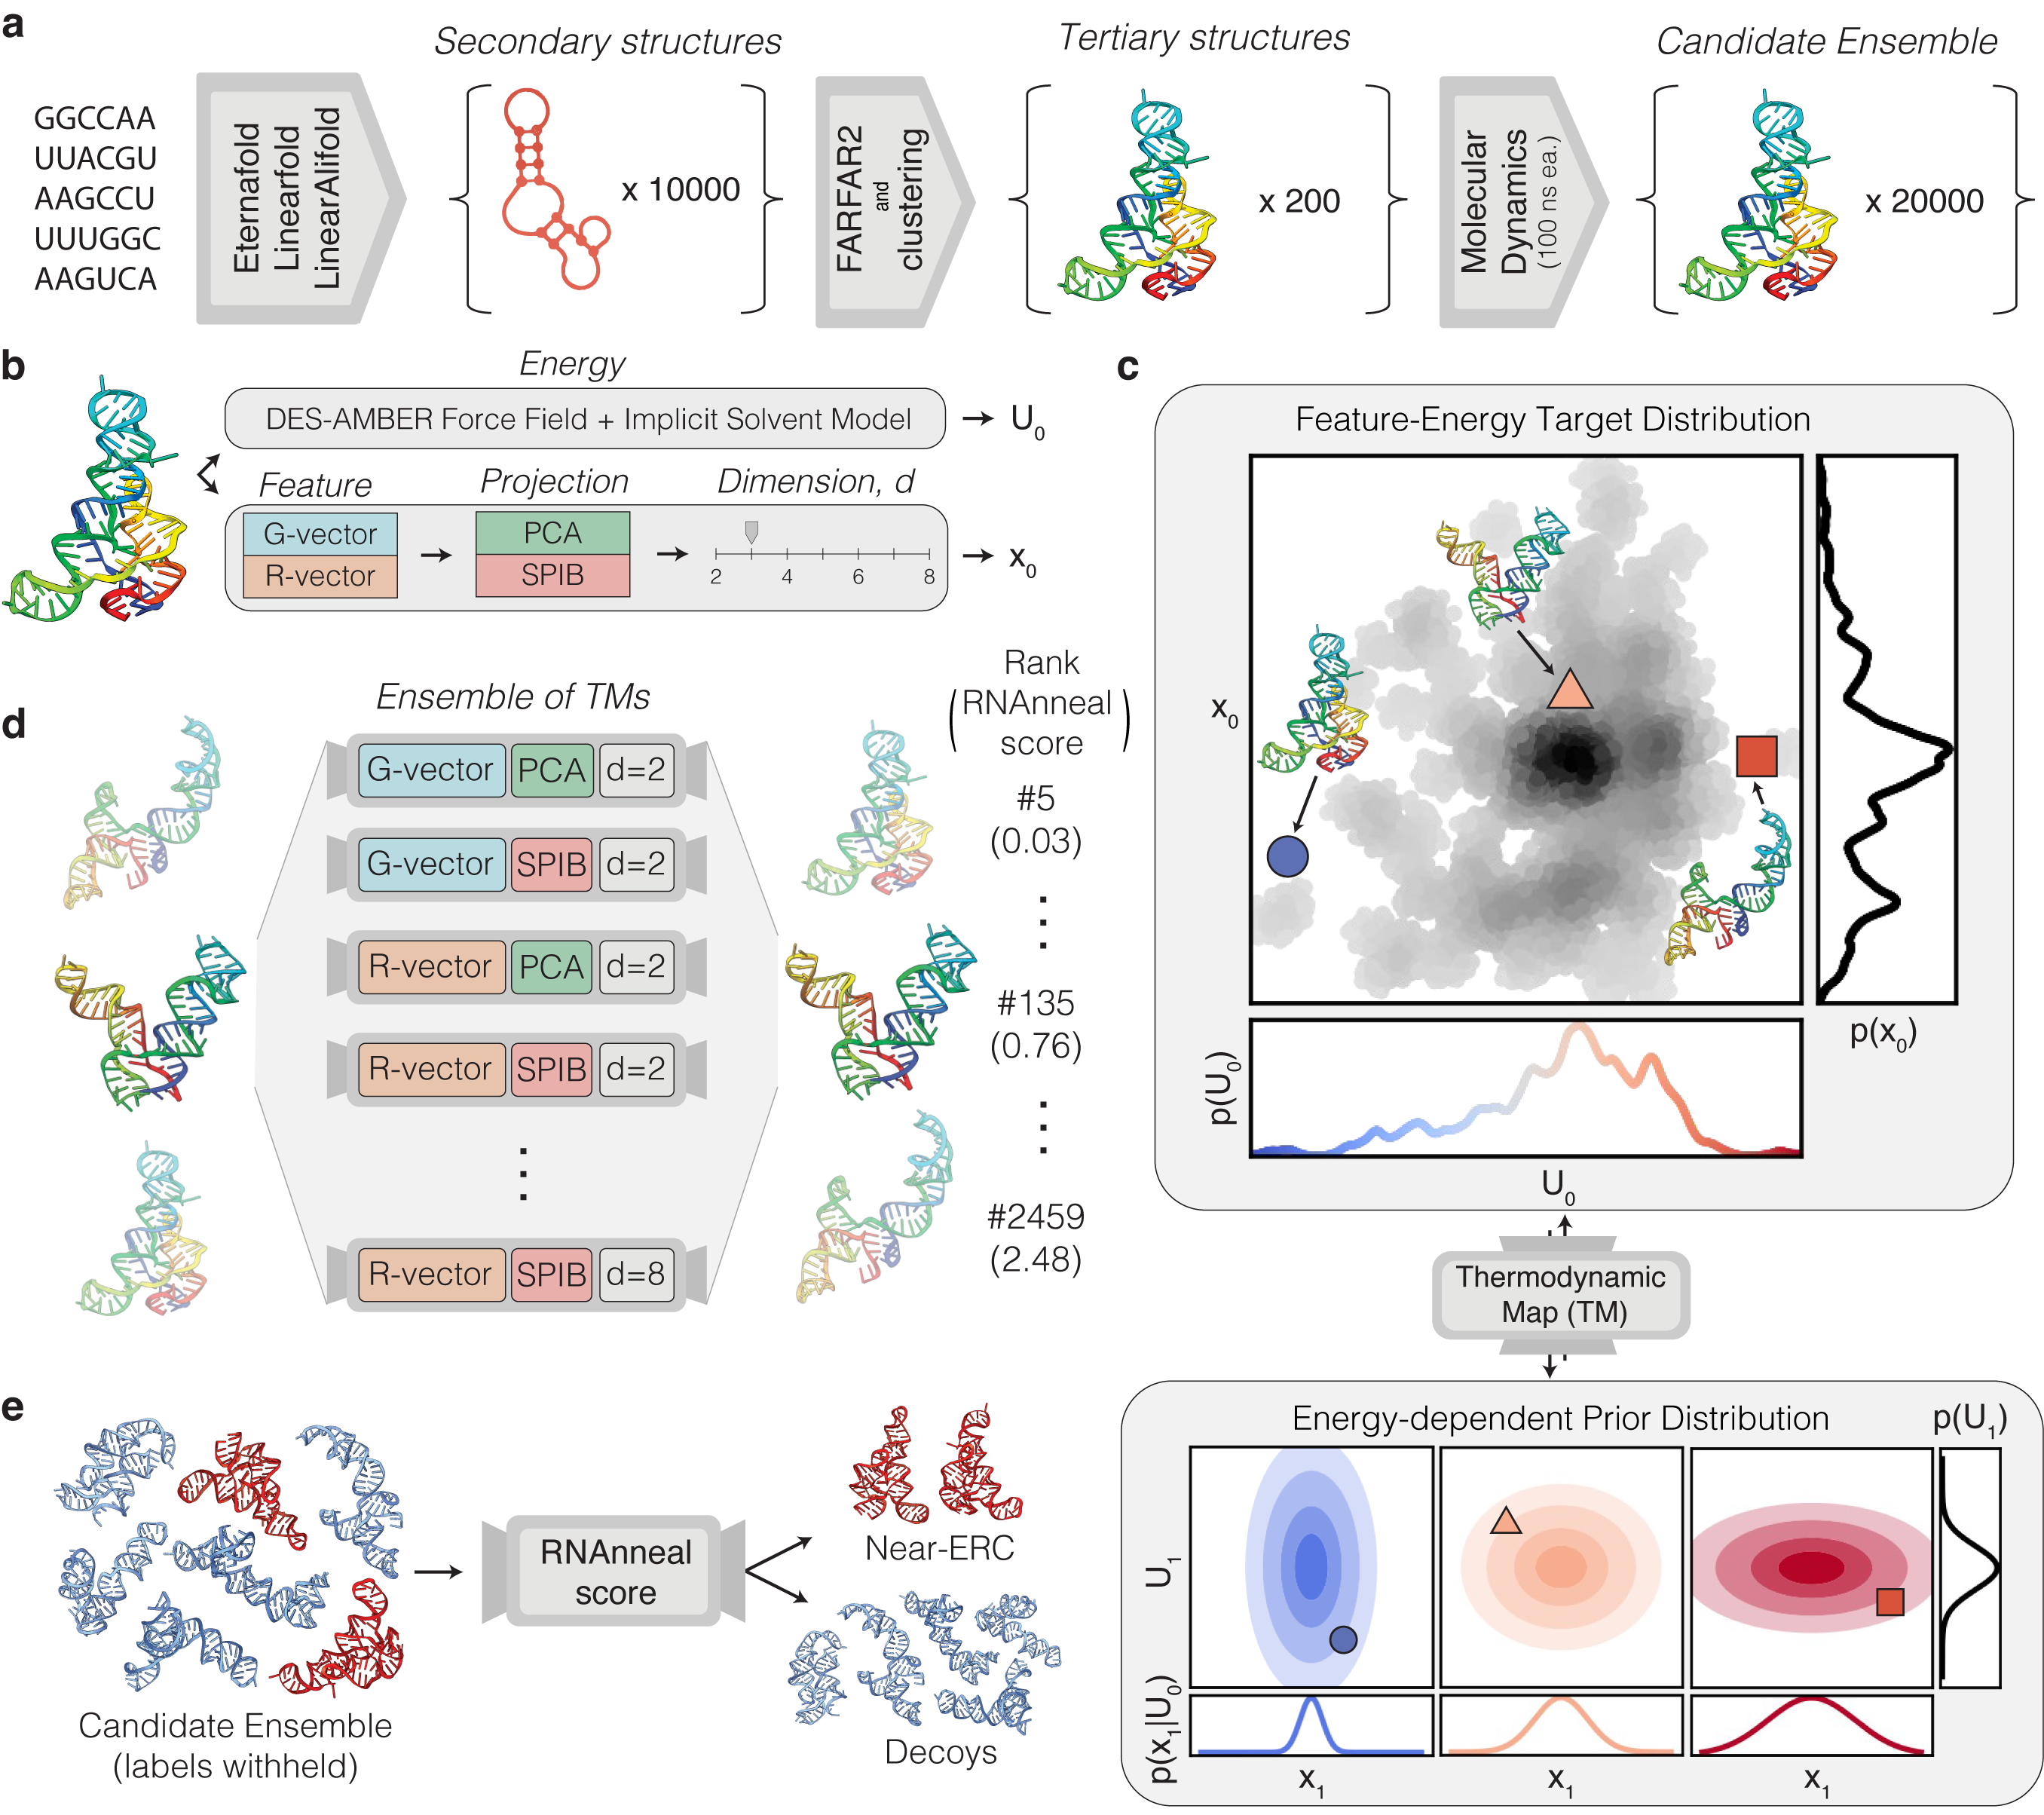
\includegraphics[
    width=1\textwidth
    ]{./schematic-1.png}
    \caption{{\bf Illustrative overview of RNAnneal.} {\bf a.} The conformational sampling component of RNAnneal is illustrated. Starting with the primary sequence, a large number of secondary and tertiary structures are predicted in succession. The tertiary conformations are clustered into, e.g., 200 conformations, before being simulated for 100ns each. Together, the simulation frames form a set of diverse candidate conformations that will be scored by RNAnneal. {\bf b.} Energetic features (upper track) and latent representations (lower track) are extracted from each conformation. {\bf c.} The structure of a thermodynamic map (TM) is illustrated: latent representations are mapped onto an energy-dependent prior distribution, while the energies themselves are mapped onto a unit normal distribution. {\bf d.} RNA conformations are ranked based on their RNAnneal scores, which is obtained by estimating the likelihood of each conformation's latent representation under the trained TM models. {\bf e.} The RNAnneal score is suited for the task of classifying realistic RNA structures from decoys.}
    \label{fig:schematic}%
\end{figure*}

RNAnneal approaches structure prediction as a needle-in-a-haystack classification problem. The first step involves thoroughly sampling a large set of structures which we assume contains both realistic and decoy conformations (Fig. \ref{fig:schematic}a and Fig. \ref{fig:results}a-f). Structure prediction then amounts to distinguishing realistic structures from the decoys (Fig. \ref{fig:schematic}e). To accomplish this, we develop the RNAnneal score, which is parameterized by an ensemble of deep-learning models (Fig. \ref{fig:schematic}b-e). In our evaluations, we show that the RNAnneal score effectively prioritizes experimentally-resolved conformations (ERCs) over decoys and use the score to predict weighted ensembles of representative structures for 15 riboswitch RNAs (Fig. \ref{fig:results}i-k).

The first step of RNAnneal consists of sampling a set of candidate conformations (Fig. \ref{fig:schematic}a). With only the primary sequence as input, we employ three programs to generate a large number of secondary structures (Eternafold, Linearfold and LinearAlifold; see {\nameref{methods:sec-struct}), which are then assembled into all-atom tertiary models using the FARFAR2 algorithm (see \nameref{methods:tertiary-struct}).\cite{huang2019linearfold,wayment2022rna,malik2024linearalifold,watkins2020farfar2} Next, 200 diverse, representative models of the tertiary structure are selected by clustering on geometric features and ranking conformations based on their Rosetta scores (see  \nameref{methods:representatives}). To produce a final set of candidate structures, each of the representative conformations is simulated for 100ns via implicit solvent molecular dynamics (MD; see \nameref{methods:molecular-dynamics}) . 

The second stage of RNAnneal involves extracting geometric features (see \nameref{methods:rna-features}) and energies (see \nameref{methods:molecular-dynamics}) from the candidate conformations in order to train an ensemble of probabilistic generative models. The geometric features are encoded as latent representations, by either Principal Component Analysis (PCA) or a State Predictive Information Bottleneck (see \nameref{methods:spib}) model.\cite{wang2021state} Then, an ensemble of Thermodynamic Maps (see \nameref{methods:thermodynamic-map}) is trained to estimate the log-likelihood of the candidate conformations based on their energies and latent representations (Fig. \ref{fig:schematic}c).\cite{herron2024inferring} TMs, which employ the powerful diffusion framework, have been shown to accurately predict molecular equilibrium distributions from sparse data collected across different thermodynamic conditions. \cite{herron2024inferring,lee2025exponentially,beyerle2025inferring} In this work, we train $28$ TMs on combinations of features (R- and G-vectors) and projections (SPIB and PCA) with 2 to 8 latent dimensions, $d$ (Fig. \ref{fig:schematic}d). It is worth noting that the energy values are consistent across all models, even though the latent representations of a given conformation vary from model to model. Finally, for a given conformation, the TM log-likelihoods are averaged to produce the RNAnneal score (see \nameref{sec:rnanneal}). Our evaluations show that the RNAnneal score can reliably distinguish between ERCs and decoys (Fig. \ref{fig:schematic}e and Fig. \ref{fig:results}c-d). 

\begin{figure*}[htbp!]
    \centering
    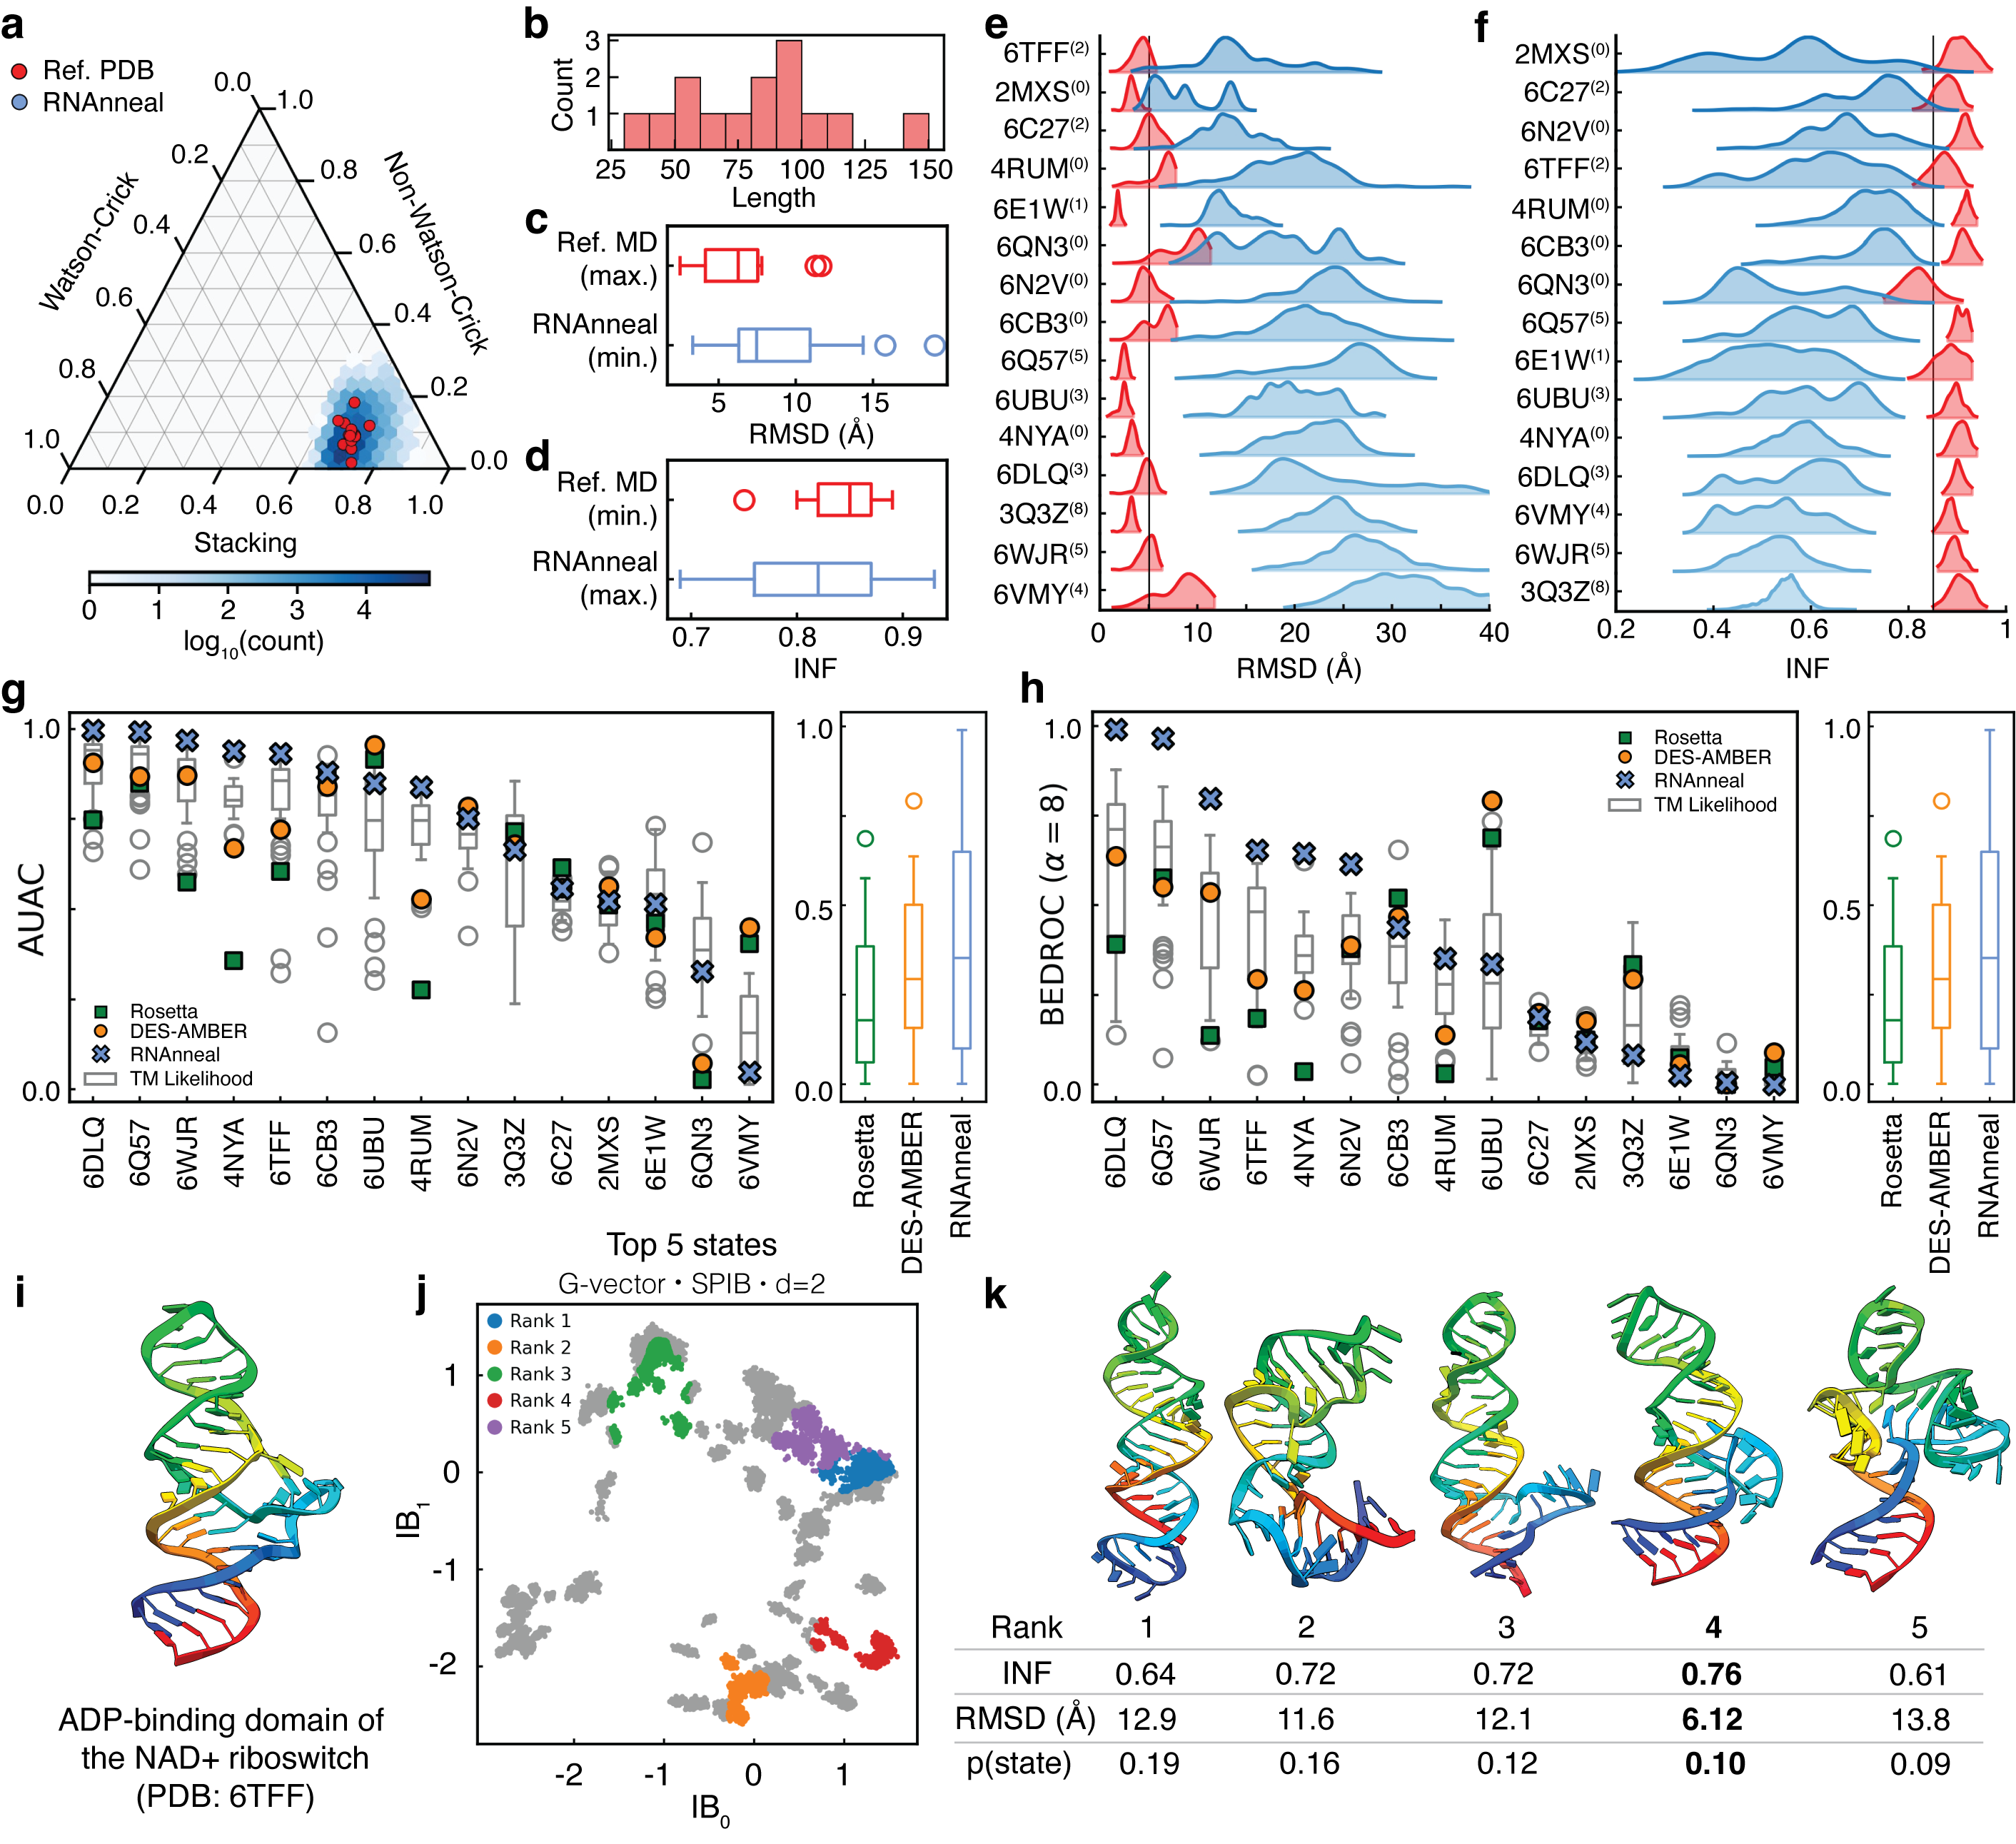
\includegraphics[
    width=\textwidth
    ]{./main-results-scaled.png}
    
    \caption{{\bf RNAnneal evaluated on the riboswitch dataset.} {\bf a.} Comparison between the interaction composition of reference (red) and RNAnneal (blue) conformations. {\bf b.} Distribution of sequence lengths for the riboswitch set. {\bf c.} Maximum RMSD values from MD simulations of the reference conformation are compared to the minimum RMSD among the RNAnneal conformations. (Median [IQR]; Ref. MD: 6.2{\AA} [$4.1-7.5${\AA}]; RNAnneal: 7.4{\AA} [$6.3-10.9${\AA}]). {\bf d.} Minimum INF values from MD simulations of the reference conformation are compared to the maximum INF among the RNAnneal conformations (Median [IQR]; Ref. MD: 0.85 [$0.82-0.87$]; RNAnneal: 0.82 [$0.76-0.87$]). {\bf e.} RMSD comparison between simulations of the reference structures and conformations predicted by RNAnneal. {\bf f.} INF comparison between simulations of the reference structure and conformations predicted by RNAnneal. Conformations with INF$\geq0.85$ (vertical line) are classified as ERCs when evaluating the RNAnneal score (panels g and h). The superscripts denote the number of pseudoknotted base pairs in the reference conformations (panels e and f). {\bf g.} Comparison of AUAC values on the structure classification task (Median (IQR); Rosetta: 0.60 [$0.43-0.76$]; DES-AMBER: 0.68 [$0.54-0.85$]; RNAnneal: 0.84 [$0.54-0.94$]). {\bf h.} Comparison of BEDROC values for the structure classification task (Median (IQR); Rosetta: 0.18 [$0.06-0.39$]; DES-AMBER: 0.29 [$0.16-0.50$]. RNAnneal: 0.35 [$0.10-0.65$]). {\bf i.} Tertiary structure of reference conformation 6TFF. {\bf j.} RNAnneal predictions for the NAD$^+$ riboswitch are projected along the information bottleneck (IB) components with the top-five states labeled. {\bf k.} Representative conformations are displayed for each of the top-five states. The state populations and INF and RMSD relative to the reference conformation (PDB: 6TFF) are also reported. Bolded states contain ERCs.}
    \label{fig:results}%
\end{figure*}


We evaluate RNAnneal's structure prediction performance on a set of 15 riboswitches originally curated in Ref.\cite{townshend2021geometric} (see \nameref{methods:preparation}; Table \ref{tab:riboswitches} and Fig. S\ref{fig:all-representatives}). Riboswitches are typically found in the 5'-untranslated region of bacterial mRNAs and are {\it cis}-acting regulatory elements that control gene expression by up- or down-regulating transcription, or, depending on class, translation.\cite{huang2025some} The basis of riboswitch function is conformational: they fold into structurally distinct ``bound'' ({\it holo}) and ``free'' ({\it apo}) states in the presence or absence of a cognate ligand, which, in turn, signals the gene expression machinery to halt or continue. Riboswitches bind their cognate ligands with high specificity through intricate structural motifs, like helix junctions, loop-loop interactions, and pseudoknots; such motifs are rich in non-WC interactions and their structures have proved challenging to model in past blind assessments.\cite{das2023assessment,bu2025rna,kretsch2025assessment} 

First, we assess if RNAnneal's conformational sampling procedure (Fig. \ref{fig:schematic}a) produces conformations that are similar to ERCs. We compared the interaction composition of conformations sampled by RNAnneal to the reference ERCs, finding that 60-80\% of interactions are stacking, 10-30\% are Watson-Crick (WC), and 0-20\% are non-WC for both sets (Fig. \ref{fig:results}a). The interaction compositions are consistent for all the ERCs, even though their lengths range from 28 to 149 nucleotides (Fig. \ref{fig:results}b). To evaluate differences between the RNAnneal and reference ERCs, we simulated each reference conformation (see \nameref{methods:molecular-dynamics}) and monitored how the Root Mean Squared Deviation (see \nameref{methods:rmsd}) and Interaction Network Fidelity (see \nameref{methods:inf}) changed over the course of the simulation (Fig. \ref{fig:results}c-f).\cite{parisien2009new} For each simulation, we examined the furthest excursion from the reference conformation as measured by the maximum RMSD (RMSD$_{\mathrm{max}}$) and minimum INF (INF$_{\mathrm{min}}$). We compared the values to the closest RNAnneal conformation, as measured by RMSD$_{\mathrm{min}}$ and INF$_{\mathrm{max}}$. The median RMSD$_{\mathrm{max}}$ among all reference structures was $6.2${\AA} and the median INF$_{\mathrm{min}}$ was $0.85$; RNAnneal sampled structurally similar conformations with a median RMSD$_{\mathrm{min}}$ of $7.4${\AA} and a median INF$_{\mathrm{max}}$ of $0.82$ (Fig. \ref{fig:results}c-d).  We computed the correlation between the INF and RMSD values of the RNAnneal conformations separately for each riboswitch and found an $r$ of $-0.50\pm0.22$ ($\mu\pm\sigma$) indicating weak correlation (Fig. S\ref{fig:correlation}). Indeed, some ERCs exhibited large changes in RMSD during simulation while still maintaining the interaction network (4RUM and 6VMY) and vice versa (6E1W and 6UBU). Nine of the ERCs contain pseudoknots, which are excluded from the secondary structure prediction algorithms we employ. Consequently, the performance of RNAnneal degrades as the number of pseudoknotted base pairs increases (superscript in Fig. \ref{fig:results}e-f). A notable exception is the NAD$^+$ riboswitch (6TFF) for which RNAnneal still sampled ERC-like (INF$\geq0.85$) conformations. RNAnneal also sampled ERC-like conformations for 6 of the 7 pseudoknot-free reference structures (2MXS, 6C27, 6N2V, 4RUM, 6CB3, and 6QN3). All together, our results indicate that RNAnneal samples realistic, pseudoknot-free RNA structures.

Next, we benchmark the performance of the RNAnneal score on the task of classifying ERCs apart from decoy conformations by comparing to two other scores: the Rosetta and DES-AMBER scores (see \nameref{methods:tertiary-struct} and \nameref{methods:molecular-dynamics}). For this evaluation, we create a new set of structures by adding conformations from the reference simulations to the pool of conformations sampled by RNAnneal, and then ordering the set based on their scores (Fig. S\ref{fig:inf_combined}). We measure how well each score prioritizes ERCs (INF $\geq 0.85$) over decoys (INF $< 0.85$) with two metrics: Area Under the Accumulation Curve (see \nameref{methods:auac}) and Boltzmann-Enhanced Discrimination of Receiver Operator Characteristic (see \nameref{methods:bedroc}).\cite{truchon2007evaluating} The AUAC is dominated by contributions from the lowest-ranked models, while BEDROC emphasizes classification accuracy among the highest-ranked structures via a tunable parameter $\alpha$. Both metrics vary from zero to one, with the latter indicating perfect classification of ERCs over decoys. On the classification task, the RNAnneal score broadly outperformed the Rosetta and DES-AMBER scores for both the AUAC and BEDROC metrics (Fig. \ref{fig:results}g-h). RNAnneal had a median AUAC of $0.84$ which was greater than the $0.68$ for DES-AMBER or $0.60$ for Rosetta. Similarly, the median BEDROC for RNAnneal was $0.35$ compared to $0.29$ for DES-AMBER or $0.18$ for Rosetta. Interestingly, when the ensemble of TM models performs well as a whole, we observe an ensemble effect where the RNAnneal score shows superior classification performance over any individual TM model (Fig. \ref{fig:results}g-h). We also found little variation in AUAC or BEDROC between different features and projections; instead, most of the variation is due to the latent dimension, $d$ (Fig. S\ref{fig:classification-by-feature}). Similar results were obtained when RMSD $\leq5${\AA} is used as a classification criteria for defining ERCs (Fig. S\ref{fig:rmsd-enrichment}).

The AUAC and BEDROC results indicate that RNAnneal prioritizes experimentally-resolved riboswitch structures over decoys. However, all but one of the reference ERCs are representative of the {\it holo} state. It is oftentimes infeasible to probe {\it apo} conformations with current high-resolution techniques due to increased conformational flexibility (i.e., heterogeneity) in the absence of a ligand. We make predictions of {\it apo} conformations for each riboswitch by ranking states predicted by SPIB based on their average RNAnneal score (see \nameref{methods:state-ranking}). We present an example prediction for the NAD$^{+}$ riboswitch: the {\it holo} ERC (6TFF) contains two pseudoknotted base-pairs that form a bulge-loop interaction, which stabilizes the otherwise disordered loop to accommodate a ligand (Fig. \ref{fig:results}i; ligand not pictured). We report an ensemble containing the top-five ranked states (Fig. \ref{fig:results}j-k). The bulge nucleotides are sequestered by base pairing in the representative conformation for the top-ranked state; the second-, third-, and fourth-ranked state representatives reflect conformational flexibility in the absence of the loop-bulge interaction; and the representative conformation for the fifth-ranked state presents an altogether different cloverleaf structure (Fig. \ref{fig:results}k). The reference structure for FMN riboswitch (6WJR) is the only {\it apo} representative in the set. Although RNAnneal failed to sample the ERC due to pseudoknotted base pairs, the RNAnneal score unambiguously selected for the ERC (Fig. \ref{fig:results}e-h). Five-state predictions are provided in Fig. S\ref{fig:rep-ensemble-1}-S\ref{fig:rep-ensemble-4} for all 15 riboswitches. 

Summarily, we have introduced in this work RNAnneal as an {\it ab initio} pipeline for RNA structure prediction and evaluation which makes no explicit use of ERCs. Nonetheless, the results of our evaluations indicate that RNAnneal accurately samples pseudoknot-free ERCs which are favored by the RNAnneal score. The strong performance of RNAnneal on structure prediction tasks may be attributed to multiple factors: our hierarchical approach to sampling of the structure ensemble, effective structure featurization, and deep-learning models that incorporate physically-motivated inductive biases. Overall, we believe that RNAnneal will enable rapid and exploratory characterization of RNA structure ensembles. Future work will expand the scope of RNAnneal's modeling by accounting for the effect of Mg$^\mathrm{2+}$ on folding, guiding conformational sampling with low-resolution structure-probing information, modeling non-canonical interactions using templates, and predicting pseudoknots.

\section*{Methods}

\subsection*{Secondary Structure Prediction}
\phantomsection
\setcurrentname{Secondary Structure Prediction}
\label{methods:sec-struct}
The secondary structure of an RNA is a simplified representation that specifies Watson-Crick base pairing. There are numerous, long-standing approaches available to predict secondary structures from the primary sequence.\cite{sato2023recent} RNAnneal relies on three programs to predict RNA secondary structures: EternaFold\cite{wayment2022rna}, LinearFold\cite{huang2019linearfold}, and LinearAliFold\cite{huang2019linearfold}. EternaFold is a probabilistic method for secondary structure prediction that
has been benchmarked against several widely used secondary structure prediction algorithms (Algorithm \ref{alg:eternafold-sampling}). LinearFold is an algorithm for predicting secondary structures that has linear runtime with sequence length (Algorithm \ref{alg:linearfold-sampling}). LinearAliFold extends the functionality of LinearFold by implementing stochastic sampling (Algorithm \ref{alg:linearalifold-sampling}). After a large number of secondary structures have been predicted by the above methods, the structures are aggregated and redundant ones are filtered out.  Fig. S\ref{fig:sec-struct-eval} measures the fraction of correctly predicted bases for the predicted distributions of secondary structures for each riboswitch. 

\subsection*{FARFAR2}
\phantomsection
\setcurrentname{FARFAR2}
\label{methods:tertiary-struct}

Rosetta's Fragment Assembly of RNA with Full-Atom Refinement (FARFAR) is a hybrid knowledge- and physics-based approach to sampling models of RNA tertiary structure.\cite{das2010atomic} FARFAR samples tertiary models by performing Monte Carlo sampling on a low-resolution potential using a library of experimentally validated structure fragments, and then relaxes the structure in a higher-resolution all-atom potential. The quality of the conformations is evaluated by the Rosetta score. FARFAR2 further improves the performance of FARFAR with updates to the sampling algorithms, scoring weights, and fragment libraries.\cite{watkins2020farfar2} The Rosetta score referred to in the main text and Fig. \ref{fig:results}g-h corresponds to the \texttt{rna\_hires.wts} file in Rosetta v2021.16.61629. Algorithm \ref{alg:rna_denovo} describes how RNAnneal uses FARFAR2 to sample a candidate model of the tertiary structure with the primary sequence and a secondary structure as input.

\subsection*{Clustering}
\phantomsection
\setcurrentname{Clustering}
\label{methods:representatives}

A crucial step in RNAnneal is selecting representative conformations to simulate (see \nameref{methods:molecular-dynamics}) from the set of structures predicted by \nameref{methods:tertiary-struct}. To sample diverse conformations, we first compute G-vectors for the FARFAR2 conformations (see \nameref{methods:rna-features}). We then project the G-vectors onto $d=2,3,\ldots,26$ principal components. For each $d$ value, we cluster the data using the advanced density peaks algorithm\cite{d2021automatic} implemented in \texttt{dadapy}\cite{glielmo2022dadapy} with $Z=3$, and select representatives based on the clustering (i.e., the $d$ value) that yields the maximum number of clusters (Fig. S\ref{fig:clusters_vs_d}). To select, e.g., 200 candidate structures, we first sort the conformations within each cluster based on their Rosetta score and then sort the clusters based on the top-scoring conformation in each cluster. The clusters are then traversed in order, and the top-scoring conformation is selected as a representative and subsequently removed from the cluster. If there are fewer than 200 candidate structures after all clusters have been traversed, then they are re-ordered based on the new top-scoring conformation and the selection procedure is repeated until 200 conformations are obtained. The entire procedure is detailed in Algorithm \ref{alg:candidate-selection}.

\subsection*{Molecular Dynamics}
\phantomsection
\setcurrentname{Molecular Dynamics}
\label{methods:molecular-dynamics}

RNAnneal simulates tertiary models of RNA structure with implicit solvent molecular dynamics in order to introduce variations in structure caused by the thermal environment. The simulations are conducted under the NVT ensemble using the OpenMM simulation engine and the DES-AMBER RNA force field.\cite{eastman2023openmm,tan2018rna} The conformations are equilibrated by gradually increasing the temperature from $1$K to $300$K and then increasing the integration timestep from $1$fs to the production integration timestep of $5$fs (Table \ref{tab:schedule}). The production simulation is 100ns and frames are saved at 1ns intervals; additional simulation parameters like ion concentration and solvent model are provided in Table \ref{tab:parameters}. The DES-AMBER score is the potential energy of the MD simulations, i.e., the energy values of the force field and solvent model, standardized by first aggregating the energy across all simulations (for a given RNA) and then subtracting the minimum value and dividing the standard deviation.

\subsection*{R- and G-vectors}
\phantomsection
\setcurrentname{R- and G-vectors}
\label{methods:rna-features}
RNAnneal featurizes conformations with two nucleobase-centric representations constructed from R- and G-vectors.\cite{bottaro2014role} An R-vector is a displacement vector $\mathbf{r}_{ij}$ directed between the six-membered aromatic ring of nucleobases $i$ and $j$. The R-representation of a conformation with $N$ nucleobases is thus a tensor of shape $N \times N \times 3$. Similarly, the G-representation is a $N \times N \times 4$
tensor consisting of G-vectors that capture the geometry of localized base-pairing and stacking interactions. The G-vector, $\mathbf{G}_{ij}$, is computed as
\begin{gather}
    \mathbf{G}_{ij}(\mathbf{r}_{ij}) = 
    \begin{pmatrix}
    \sin (\gamma \lvert \mathbf{r}_{ij}\rvert)\frac{r_{ij,x}}{\lvert \mathbf{r}_{ij}\rvert} & \\
    \sin (\gamma \lvert \mathbf{r}_{ij}\rvert)\frac{r_{ij,y}}{\lvert \mathbf{r}_{ij}\rvert} & \\
    \sin (\gamma \lvert \mathbf{r}_{ij}\rvert)\frac{r_{ij,z}}{\lvert \mathbf{r}_{ij}\rvert} &  \\
    1 + \cos (\gamma \lvert \mathbf{r}_{ij}\rvert)
    \end{pmatrix}
    \times \frac{\Theta (\lvert \mathbf{r}_{ij}\rvert - r_c)}{\gamma}
\end{gather}
where $\Theta$ is a step function, $r_c$ is a cutoff of $2.4${\AA}, and $\gamma=\pi/r_c$.

\subsection*{SPIB}
\phantomsection
\setcurrentname{SPIB}
\label{methods:spib}

The State Predictive Information Bottleneck (SPIB) framework allows one to embed a high-dimensional dynamical system into a lower-dimensional latent space while preserving the slowest degrees of freedom of the system.\cite{wang2021state} SPIB takes the form of a time-lagged autoencoder, where high dimensional coordinates at time $t$ are passed to the encoder and embedded in a latent space; the decoder must then predict the state label at time $t+\Delta t$ solely from the latent embedding. SPIB has two main hyperparameters: the time lag, $\Delta t$ and a regularizer, $\beta$. The time lag corresponds to the lifetime of the predicted states, while $\beta$ regularizes the latent space to follow a mixture of Gaussians prior. We train two sets of SPIB models on the first 8 principal components of the \nameref{methods:rna-features}. For each feature type, we train seven models with the number of IB components, $d$, ranging from 2 to 8. For all models, we use a linear encoder, non-linear decoder, a $2$ns lag time, and set $\beta=0.05$. The SPIB implementation is provided by the \texttt{af2rave} python package.\cite{teng2025alphafold2} 

% \lipsum[8]

\subsection*{TM}
\phantomsection
\setcurrentname{TM}
\label{methods:thermodynamic-map}

A thermodynamic map (TM) is a diffusion model variant that models the dependence of a structural ensemble on physical parameters like temperature, pressure, or chemical potential by representing their statistical effect on the prior distribution.\cite{herron2024inferring,lee2025exponentially,beyerle2025inferring} Temperature, for example, is represented by tempering the prior (i.e., adjusting the variance) on a per-sample basis, while pressure and chemical potential correspond to exponential tilting operations that shift the mean of the prior.\cite{herron2024inferring,lee2025exponentially} Once trained, the TM model can then be used to generate new samples or evaluate the likelihood of existing samples at a given set of thermodynamic conditions. In this work we modify the construction so that the prior is tempered based on the energy of the conformations. Intuitively, conformations that are low-lying on the energy are sampled at low temperatures, so they are mapped onto a low-variance prior, while those which are high on the energy landscape and sampled at hotter temperatures are mapped onto a high-variance prior. Concretely, for a given representation $\mathbf{x}_0$, we set the variance of the prior equal to the DES-AMBER score, $U_0$, of the conformation corresponding to $\mathbf{x}_0$ (see \nameref{methods:molecular-dynamics}; Fig. \ref{fig:schematic}c). The \nameref{sec:rnanneal} for a given conformation is computed from the log-likelihoods of the latent representations under the trained models. The log-likelihood calculation is summarized in Algorithm \ref{alg:diffusion-likelihood} and described in detail in Ref.\cite{john2025comparison} Our TM implementation infers the energy-dependence of the conformational ensemble, and as a result one must choose a variance (i.e., a temperature) for the prior when computing the score. For all the results in the main text, we employ a unit variance prior with the goal of scoring low-energy structures favorably. We found that increasing the variance of the prior during the log-likelihood calculation decreases the \nameref{methods:auac} and \nameref{methods:bedroc} values, indicating that a high-variance prior promotes diversity among the high-scoring conformations (Fig. S\ref{fig:model-temp-dependence}-S\ref{fig:acc-curve-summary}).

% A thermodynamic map (TM) is a diffusion model variant that models the dependence of a structural ensemble on physical parameters like temperature, pressure, or chemical potential by representing these parameters in the prior distribution.\cite{herron2024inferring,lee2025exponentially,beyerle2025inferring} The TM model can then be used to generate new samples or evaluate the likelihood of existing samples at a given temperature. In Ref. \cite{herron2024inferring}, for example, structures observed at a low temperature are mapped onto a prior with a small variance (i.e., a low temperature) while high-temperature samples are mapped onto a prior with large variance. In this work we modify the construction so that the TM encodes both the free- and potential-energy landscape of an RNA molecule: conformations that are low-lying on the energy landscape are mapped onto a low-variance prior, while those high on the energy landscape are mapped onto a high-variance prior. More concretely, for a given representation $\mathbf{x}_0$, we set the variance of the prior equal to the DES-AMBER score, $U_0$, of the conformation corresponding to $\mathbf{x}_0$ (see \nameref{methods:molecular-dynamics}; Fig. \ref{fig:schematic}c). The \nameref{sec:rnanneal} for a given conformation is computed from the log-likelihoods of the latent representations under the trained models. The log-likelihood calculation is summarized in Algorithm \ref{alg:diffusion-likelihood} and described in detail in Ref.\cite{john2025comparison} Evaluating the log-likelihood requires choosing a variance for the prior; all of the results reported in the main text are generated at $T=1$, but we found the RNAnneal score to be robust with respect to choice of $T$ (Fig. S\ref{fig:model-temp-dependence}-S\ref{fig:acc-curve-summary}).


\subsection*{RNAnneal Score}
\phantomsection       
\setcurrentname{RNAnneal Score} 
\label{sec:rnanneal}            

RNAnneal scores conformations using an ensemble of thermodynamics maps (\nameref{methods:thermodynamic-map}s) trained on geometric and energetic features extracted from a set of tertiary conformations (Fig. \ref{fig:schematic}b-d). A total of 28 TMs are trained for each RNA, covering all four combinations of representations (\nameref{methods:rna-features}) and projections (PCA and \nameref{methods:spib}). For each feature-projection combination, the number of projection components $d$ varies from 2 to 8 inclusive. After training, the RNAnneal score is computed from the log-likelihoods of the training data under the TM ensemble (Algorithm \ref{alg:diffusion-likelihood} and \ref{alg:rnanneal-score}).

\subsection*{Reference Structures}
\phantomsection       
\setcurrentname{Reference Structures}
\label{methods:preparation}

We evaluated RNAnneal's structure prediction performance on a set of riboswitch sequences with structures that have been solved by high-resolution experimental methods (Table \ref{tab:riboswitches} and Fig. S\ref{fig:all-representatives}). The reference ERCs were prepared by downloading the associated Protein Data Bank (PDB) entry, removing any non-nucleic residues, filling in missing nucleobases using \nameref{methods:tertiary-struct}, and subsequently minimizing the conformation with the Rosetta energy function (see Algorithm \ref{alg:farfar-minimise}).

\subsection*{RMSD}
\phantomsection       
\setcurrentname{RMSD}
\label{methods:rmsd}

Root Mean Squared Deviation (RMSD) is a metric commonly used to evaluate discrepancies between structure models. We evaluate the heavy-atom RMSD of each model after alignment to the native structure. The RMSD between a model $\mathbf{x}$ and reference $\mathbf{y}$ conformation containing $N$ heavy atoms is defined as
\begin{equation}
    \mathrm{RMSD}(\mathbf{x}, \mathbf{y}) = \sqrt{\frac{1}{N}\sum_{i=1}^N d(\mathbf{x}_i, \mathbf{y}_i)^2},
\end{equation}
where $d(\mathbf{x}_i, \mathbf{y}_i)$ measures the distance between the $i$-th atom in both models. The RMSD values for RNAnneal conformations and molecular dynamics simulations of the reference structure are reported in Fig. S\ref{fig:rmsd_decoys} and Fig. S\ref{fig:rmsd_reference}. 

\subsection*{INF}
\phantomsection       \setcurrentname{INF}
\label{methods:inf}

Interaction Network Fidelity (INF) measures structural discrepancy between two conformations in terms of their Leontis-Westhof base pairing and stacking classifications.\cite{parisien2009new} Intuitively, the INF is the Matthews correlation coefficient between the classified interactions in a model and reference structure. An INF of zero indicates that there are no common interactions between the model and reference structures, while an INF of one indicates identical structures. Relatively minor, localized differences in structure (e.g. at a helix junction) may result in a large RMSD due to poor alignment between the model and reference conformation. The INF does not require alignment and is therefore more robust to minor variations in structure caused by thermal fluctuations. We compute the INF using the ClaRNA\cite{walen2014clarna} implementation in \texttt{rna-tools}\cite{magnus2020rna}. The INF values for RNAnneal conformations and molecular dynamics simulations of the reference structures are reported in Fig. S\ref{fig:inf-detailed} and S\ref{fig:inf_reference}-\ref{fig:inf_decoys}.

\subsection*{AUAC}
\phantomsection       \setcurrentname{AUAC}
\label{methods:auac}
The Area Under the Accumulation Curve (AUAC) is a metric suited for evaluating classification task performance (Fig. \ref{fig:schematic}e and \ref{fig:results}g).\cite{truchon2007evaluating} Let $x\in [0,1]$ be the normalized rank and $f:x \rightarrow \{0,1\}$ be an associated set of labels, with $1$ indicating the positive (native-like) class and $0$ indicating the decoy class. The empirical CDF is then
\begin{equation}
    F(x) = \int_0^x f(s)ds
\end{equation}
and the area under the accumulation curve is 
\begin{equation}
    \label{eq:auac}
    \mathrm{AUAC} = \int_0^1 F(x)dx.
\end{equation}
When the $\mathrm{AUAC}$ is $1$, the classification is perfect, i.e., members of the positive class are always ranked above decoys. The accumulation curves for the 15 riboswitches investigated in the main text are provided in Fig. S\ref{fig:acc-curves} and S\ref{fig:acc-curve-summary}.

\subsection*{BEDROC}
\phantomsection       \setcurrentname{BEDROC}
\label{methods:bedroc}


The Boltzmann-Enhanced Discrimination of Receiver Operator Characteristic (BEDROC) modifies the Area Under the Accumulation Curve (\nameref{methods:auac}) to focus on early recognition of the positive (reference-like) class (Fig. \ref{fig:schematic}e and \ref{fig:results}g).\cite{truchon2007evaluating} The AUAC is skewed towards late recognition since contributions from the lowest ranked samples dominate the area calculation in Eq. \ref{eq:auac}. One may introduce an exponentially decreasing weight on the rank in the AUAC calculation to focus on early recognition, i.e.,
\begin{equation}
    \label{eq:wauac}
    w\mathrm{AUAC} = \int_0^1 F(x)e^{-\alpha x}dx,
\end{equation}
which is normalized to obtain
\begin{equation}
    \label{eq:bedroc}
    \mathrm{BEDROC} = \frac{w\mathrm{AUAC} - w\mathrm{AUAC}_{\mathrm{min}}}{w\mathrm{AUAC}_{\mathrm{max}} - w\mathrm{AUAC}_{\mathrm{min}}}.
\end{equation}
The tunable parameter $\alpha$ controls the focus on early recognition. Our choice of $\alpha=8$ is such that the top $20\%$ of the normalized rank contributes $80\%$ of the $w\mathrm{AUAC}$. Early recognition is a suitable evaluation metric when there is a large class imbalance and accurate classification among the highest ranks is essential.

\subsection*{State Ranking}
\phantomsection       \setcurrentname{State Ranking}
\label{methods:state-ranking}

We briefly describe the procedure by which a conformational ensemble, i.e., a small number of representative conformations and their weights, is predicted by RNAnneal. We project the RNAnneal conformations onto the $d=2$ information‑bottleneck (IB) space learned by \nameref{methods:spib} to obtain latent representations $\{\mathbf{x}_0,\mathbf{x}_1,\ldots,\mathbf{x}_N\}$. We further assign the predicted state label, $y_i \in \{y_0,y_1,\ldots,y_M \}$ and \nameref{sec:rnanneal}, $s_i$, to each conformation. Next, we histogram the conformations on a $K \times L$ grid in the IB space (Fig. \ref{fig:results}j), using the mean $s$ in each bin (denoted by $\overline{{s}}_{kl}$) to define a Boltzmann‑like weight
$w_{kl} = \exp[{-\overline{{s}}_{kl}}]$. We assign each populated bin a state label, $y_{kl}$, based on the most frequent state label of the conformations in the bin, and define a total weight, $W_i$, for state $y_i$ by $W_i = \sum_{y_{kl}=y_i} w_{kl}$. Finally, normalizing the state weights yields state probabilities $p_{yi}$, and the frame with the minimal $s_i$ within each state is taken as its representative conformation. The entire procedure is described in Algorithm \ref{alg:state-ranking}. The states predicted in the main text (Fig. \ref{fig:results}i-k) and supplement (Fig. S\ref{fig:rep-ensemble-1}-S\ref{fig:rep-ensemble-4}) were predicted based on a $d=2$ SPIB model trained on the first 8 PCA components of the G-vectors. 

% \subsection{Structure of a Thermodynamic Map}

% The structure of the map is best understood through superstatistics -- an extension of Gibbs-Boltzmann statistics where fluctuations of intensive variables are permitted. In examining $p(\mathbf{x}_1)$ as the marginal of $p(\mathbf{x}_1, \mathbf{x}_0)$ one finds
% \begin{align}
%     p(\mathbf{x}_1) =& \int p(\mathbf{x}_1, \mathbf{x}_0) d \mathbf{x}_0 \\
%     =& \int p(\mathbf{x}_1| \mathbf{x}_0) r(\mathbf{x}_0) d \mathbf{x}_0 \\
%     p(\mathbf{x}_1) = & \int \frac{\exp \left[{-U_1(\mathbf{x}_1)/U_0(\mathbf{x}_0)}\right]}{Z(\mathbf{x}_0)} r(\mathbf{x}_0) d\mathbf{x}_0
% \end{align}
% which amounts to Beck and Cohen's superstatistic
% \begin{align}
%     p(\mathbf{x}_1) =& \int_0^\infty \exp \left[ {-\beta U_1(\mathbf{x}_1)} \right] f(\beta) d\beta
% \end{align}
% after the change of variables
% \begin{equation}
%     f(\beta) = \int \frac{r(\mathbf{x}_0)}{Z(\mathbf{x}_0)} \delta\left( \beta - \frac{1}{U_0(\mathbf{x}_0)}\right) d \mathbf{x}_0.
% \end{equation}
% The prior is a superposition of the Gibbs-Boltzmann statistic $\exp \left[-\beta U_1(\mathbf{x}_1) \right]$ and inverse-temperatures $f(\beta)$. In superstatistics $f(\beta)$ is often modeled analytically as a gamma or log-normal distribution, but in our case the distribution is determined by the data $\mathbf{x}_0 \in \mathcal{D}$. Since our score model is trained jointly on $f(\beta)$ and $r(\mathbf{x}_0)$, one may sample $p_\theta(\mathbf{x}_0, \beta_0)$ by first sampling $\mathbf{x}_1 \propto \exp \left[ {-\beta U_1(\mathbf{x})} \right]$ and $\beta_1 \propto \exp \left(-\beta^2/2 \right)$ and then simulating the dynamics in Eq. \ref{eq:sde-bck}.


% \lipsum[8]

% \subsection*{Boltzmann-Enhanced Discrimination of Receiver Operator Characteristic (BEDROC)}

% \lipsum[8]

% \bibliographystyle{aip}
\bibliography{main}
\clearpage
\onecolumngrid


\section*{Supplementary Information}

\begin{algorithm}[H]
  \caption{Sampling RNA Secondary Structures with \texttt{EternaFold}}
  \label{alg:eternafold-sampling}
  \begin{algorithmic}[1]
    \REQUIRE \texttt{example.fa} (input sequence);\\
    \texttt{N} (maximum number of samples, \texttt{5000})
    \STATE \texttt{mkdir -p eternafold}
    \STATE \texttt{EternaFold/src/contrafold sample example.fa} \\
    \ \texttt{--params EternaFold/parameters/EternaFoldParams.v1} \\
    \ \texttt{--nsamples N > eternafold/ef.ss}
  \end{algorithmic}
\end{algorithm}

\begin{algorithm}[H]
  \caption{Sampling RNA Secondary Structures with \texttt{LinearFold}}
  \label{alg:linearfold-sampling}
  \begin{algorithmic}[1]
    \REQUIRE \texttt{example.fa} (input sequence)
    \STATE \texttt{mkdir -p linearfold-v}
    \COMMENT {Vienna parameters}
    \STATE \texttt{mkdir -p linearfold-c}
    \COMMENT {CONTRAfold parameters}
    \STATE \texttt{cat example.fa | linearfold --zuker --delta 1000 -V | tail -n +5 | awk '\{print \$1\}' > linearfold-v/zuker.ss} \\
    \STATE \texttt{cat example.fa | linearfold --zuker --delta 1000       | tail -n +5 | awk '\{print \$1\}' > linearfold-c/zuker.ss}
  \end{algorithmic}
\end{algorithm}

\begin{algorithm}[H]
  \caption{Sampling RNA Secondary Structures with \texttt{LinearAliFold}}
  \label{alg:linearalifold-sampling}
  \begin{algorithmic}[1]
    \REQUIRE \texttt{example.fa} (input sequence);\\
    \texttt{N} (maximum number of samples, \texttt{20000})
    \STATE \texttt{mkdir -p linearalifold-v}
    \COMMENT {Vienna parameters}
    \STATE \texttt{mkdir -p linearalifold-bl}
    \COMMENT {BL* parameters}

    \STATE \texttt{cat example.fa | linearalifold.py -s N -e 1 > linearalifold-v/stochastic.ss}
    \STATE \texttt{cat example.fa | linearalifold.py -s N -e 2 > linearalifold-bl/stochastic.ss}
    \STATE \texttt{cat example.fa | linearalifold.py -p -B linearalifold-v/bpp.txt -M linearalifold-v/mea.ss -T linearalifold-v/threshknot.ss -C linearalifold-v/centroid.ss -e 1}
    \STATE \texttt{cat example.fa | linearalifold.py -p -B linearalifold-bl/bpp.txt -M linearalifold-bl/mea.ss -T linearalifold-bl/threshknot.ss -C linearalifold-bl/centroid.ss -e 2}
  \end{algorithmic}
\end{algorithm}

\begin{algorithm}[H]
  \caption{Conformational Sampling with FARFAR2}
  \label{alg:rna_denovo}
  \begin{algorithmic}[1]
  \REQUIRE \texttt{SEQ} (input sequence);\\
  \texttt{DB} (secondary structure in dot-bracket notation)
    \STATE \texttt{rna\_denovo.default.linuxgccrelease} \\
    \ \texttt{-sequence SEQ} \COMMENT {From \texttt{example.fa} in Algorithms \ref{alg:eternafold-sampling}-\ref{alg:linearalifold-sampling}} \\
    \ \texttt{-secstruct DB} \COMMENT {\texttt{cat */*.ss | uniq} from Algorithms \ref{alg:eternafold-sampling}-\ref{alg:linearalifold-sampling}}\\
    \ \texttt{-nstruct 1} \\
    \ \texttt{-cycles 20000} \\
    \ \texttt{-minimize\_rna true} \\
    \ \texttt{-rna:denovo:rounds 10} \\
    \ \texttt{-rna:denovo:minimize:minimize\_bps true} \\
    \ \texttt{-rna:denovo:bps\_moves true}
  \end{algorithmic}
\end{algorithm}

\begin{algorithm}[H]
  \caption{Reference conformation Preparation with FARFAR2}
  \label{alg:farfar-minimise}
  \begin{algorithmic}[1]
    \REQUIRE \texttt{SEQ} (input sequence);\\
    \texttt{REF} (reference PDB file)
    \STATE \texttt{rna\_denovo.default.linuxgccrelease} \\
    \ \texttt{-sequence \$(echo \$SEQ)} \COMMENT{lower‑case sequence} \\[-0.2em]
    \ \texttt{-secstruct '.....'} \COMMENT{all bases unpaired; equal to length of \texttt{\$SEQ}} \\[-0.2em]
    \ \texttt{-nstruct 1} \\[-0.2em]
    \ \texttt{-out:file:silent \$(dirname \$REF)/silent.out} \\[-0.2em]
    \ \texttt{-s \$REF} \COMMENT{experimental model} \\[-0.2em]
    \ \texttt{-minimize\_rna true} \\[-0.2em]
    \ \texttt{-rna:denovo:rounds 1} \\[-0.2em]
    \ \texttt{-out:overwrite true} \\[-0.2em]
    \ \texttt{-cycles 10000} \\[-0.2em]
    \ \texttt{-rna:denovo:minimize:minimize\_bps true}
  \end{algorithmic}
\end{algorithm}

\begin{algorithm}[H]
  \caption{Unsupervised Selection of Diverse Candidate conformations}
  \label{alg:candidate-selection}
  \begin{algorithmic}[1]
    \REQUIRE FARFAR2 models $\{\mathbf{x}_i\}_{i=1}^{N}$; \\
    Density‐peaks parameter $Z{=}3$;\\
    Principal-component range $d\!=\!2,3\ldots\,26$;\\
    Target count $K{=}200$
    \STATE Featurize each model $\mathbf{x}_i$ into a G-vector
    \FOR{$d \in \{2,3,\dots,26\}$}
      \STATE Project all G-vectors onto the first $d$ principal components
      \STATE Cluster the projection with \texttt{dadapy} (advanced density peaks, $Z{=}3$)
      \STATE Record the number of clusters obtained
    \ENDFOR
    \STATE Let $d^\ast$ be the dimension giving the maximum cluster count \COMMENT{see Fig.\,S\ref{fig:clusters_vs_d}}
    \STATE Re-cluster the $d^\ast$-dimensional data to obtain $\{\mathcal{C}_j\}_{j=1}^{M}$
    \FORALL{clusters $\mathcal{C}_j$}
      \STATE Sort conformations in $\mathcal{C}_j$ by ascending Rosetta score
    \ENDFOR
    \STATE Sort the clusters by the best Rosetta score among all conformations in each cluster
    \STATE $\mathcal{S} \leftarrow \varnothing$ \COMMENT{set of selected candidates}
    \WHILE{$|\mathcal{S}| < K$}
      \FOR{$j = 1$ \TO $M$}
        \IF{$\mathcal{C}_j \neq \varnothing$}
          \STATE Remove the top-scoring conformation $c$ from $\mathcal{C}_j$ and add $c$ to $\mathcal{S}$
          \IF{$|\mathcal{S}| = K$}
            \STATE \textbf{break}
          \ENDIF
        \ENDIF
      \ENDFOR
      \STATE Re-sort clusters by their current top-scoring conformation
    \ENDWHILE
    \RETURN $\mathcal{S}$ \COMMENT{200 candidate conformations}
  \end{algorithmic}
\end{algorithm}

\begin{algorithm}[H]
  \caption{Likelihood Estimation for a Thermodynamic Map (Diffusion Model) using the Hutchinson Trace Estimator}
  \label{alg:diffusion-likelihood}
  \begin{algorithmic}[1]
    \REQUIRE Observed frame $\mathbf{u}_{0}\equiv (\mathbf{x}_0, U_0)^\top$ (data at $t_0\equiv t={0}$); \\
    Diffusion process $\mathcal{D}$ with time grid $\{t_{0}\!\!<\!\!t_{1}\!\!<\!\!\dots\!\!<\!\!t_{K}\}$; \\
    One–step map $\mathrm{STEP}_{t_{k}\!\rightarrow t_{k+1}} \colon \mathbf{u}\!\mapsto\!\mathbf{u}'$; \COMMENT{Neural network} \\
    Prior temperature $T$; \COMMENT{$T=1$ unless otherwise stated} \\
    Temperature-dependent prior density $q_T(\mathbf{u}_{t_K})\equiv \mathcal{N}(0,T) \times \mathcal{N}(0,1)$; \COMMENT{Different priors for $\mathbf{x}$ and $U$} \\
    Schedule of noise scales $\{\beta_{k}\}_{k=1}^{K}$; \\
    Number of Hutchinson probe vectors $M$
    \STATE $\mathbf{u}\leftarrow\mathbf{u}_{0}$  \COMMENT{state at the current time $t_{k}$}
    \STATE $\mathcal{G}\leftarrow[\,]$          \COMMENT{to store divergence $g_{k}$}
    \FOR{$k\;=\;0\;\mathbf{to}\;K-1$}
      \STATE Draw $M$ probe vectors
             $\bigl\{\mathbf{v}^{(m)}\bigr\}_{m=1}^{M}
                    \sim\mathcal{N}\bigl(\mathbf{0},\mathbf{I}\bigr)$
      \FORALL{probes $m=1,\dots,M$}
        \STATE $(\mathbf{u}'^{(m)},\mathbf{Jv}^{(m)})\;
               \leftarrow\;
               \mathrm{JVP}\Bigl(
                 \mathrm{STEP}_{t_{k}\!\rightarrow t_{k+1}},
                 \mathbf{u},\,
                 \mathbf{v}^{(m)}
               \Bigr)$ \COMMENT{Jacobian‐vector product}
      \ENDFOR
      \STATE $\displaystyle
             g_{k}\;\leftarrow\;
             \frac{1}{M}
             \sum_{m=1}^{M}
               \bigl\langle
                 \mathbf{Jv}^{(m)},\,\mathbf{v}^{(m)}
               \bigr\rangle$
             \COMMENT{Hutchinson trace estimate of $\nabla_{\!\mathbf{u}}\!\cdot\!\mathrm{STEP}$}
      \STATE Append $g_{k}$ to $\mathcal{G}$
      \STATE $\mathbf{u}\leftarrow\mathbf{u}'^{(1)}$ \COMMENT{all probes have the same output}
    \ENDFOR

    \STATE $\displaystyle
           \Delta \l_{pq}
           \leftarrow
           \operatorname{trapz}\bigl(\mathcal{G},\,
                                    \{\beta_{k}\}_{k=1}^{K}\bigr)$
           \COMMENT{trapezoidal integration on $(g_{k},\beta_{k})$}
    \STATE $\displaystyle
           \log q
           \leftarrow
           \log q_T\bigl(\mathbf{u}\bigr)$
           \COMMENT{prior log‐density at $t_{K}$ at temperature $T$}
    \STATE $\displaystyle
           \log p_{\theta}\bigl(\mathbf{u}_{0}\bigr)
           \leftarrow
           \log q + \Delta_{pq}$
    \RETURN $\log p_{\theta}(\mathbf{u}_{0})$
  \end{algorithmic}
\end{algorithm}

\begin{algorithm}[H]
  \caption{RNAnneal Score}
  \label{alg:rnanneal-score}
  \begin{algorithmic}[1]
    \REQUIRE  
    Log-likelihoods $\{L_{i}^{(\mathcal{F})}\}$;\\
    Feature sets $\mathcal{F}=\{\text{G-vector},\text{R-vector}\}\times\{\text{PCA},\text{SPIB}\}$;\\
    Component range $\mathcal{D}=2,3,\ldots,8$

    \STATE $\displaystyle L_{\min}\leftarrow\min_{i}L_{i}$,\quad 
           $\displaystyle\sigma_{L}\leftarrow\sqrt{\operatorname{Var}\{L_{i}\}}$
    \FORALL{frames $i$}
      \STATE $\displaystyle l_{i}\;\leftarrow\;
              {\bigl(L_{i}-L_{\min}\bigr)}\;
              {/\;\sigma_{L}}$ \COMMENT{subtract min and divide by SD}
    \ENDFOR
      \STATE Sort $\{l_{i}\}$ in ascending order
      \STATE Initialize lists $\mathcal{S} = [\,]$ and $\mathcal{L} = [\,]$
    \FORALL{confrmers $i$}
    
        \STATE $\mathcal{L}(i)\gets[\,]$
        \FORALL{feature-projection pairs $(v,f)\in\mathcal{F}$}
          \FORALL{dimensions $d\in\mathcal{D}$}
              \STATE Append $l_{i}^{(v,f,d)}$ to $\mathcal{L}(i)$
            \ENDFOR
          \ENDFOR
        \STATE Append {$\displaystyle\bar{s}_{i}
               = \frac{1}{|\mathcal{L}(i)|}\sum_{l\in\mathcal{L}(i)}l$} to ${\mathcal{S}}(i)$
               \COMMENT{{RNAnneal Score}}
       
      \ENDFOR
      \RETURN ${\mathcal{S}}(i)$
  \end{algorithmic}
\end{algorithm}



\begin{algorithm}[H]
  \caption{Boltzmann‑weighted State Ranking and Representative Selection}
  \label{alg:state-ranking}
  \begin{algorithmic}[1]
    \REQUIRE\ SPIB projections $\{\mathbf{x}_{i}\}$;\\
    State labels $\{y_{i}\}$;\\
    RNAnneal scores $\{s_{i}\}$;\\ Frame keys $\{f_{i}\}$;\\ Histogram grid size $(K=25,L=25)$;\\ Minimum population $N_{\min}=5$;\\ Pre‑filter count $k_{\mathrm{top}}=15$;\\ Report count $k_{\mathrm{rep}}=5$
    \STATE $\mathcal{F}\!\leftarrow\!\{(y_{i},\mathbf{x}_{i},s_{i},f_{i})\}$ 
    \STATE Group $\mathcal{F}$ by state label to obtain $\{\mathcal{F}_y\}$
    \STATE Discard states with $|\mathcal{F}_y|<N_{\min}$
    \STATE Compute the average score $\bar{s}_y $ for every surviving state
    \STATE Keep the $k_{\mathrm{top}}$ states with the lowest $\bar{s}_y$
    \STATE Initialise histogram $H$ on an $K\times L$ grid over 2D IB space
    \FORALL{frames $(y,\mathbf{x},s,f)\in\bigcup\mathcal{F}_y$}
      \STATE Increment $H$ at the bin containing $\mathbf{x}$ with $(s,y)$
    \ENDFOR
    \FORALL{occupied bins $(k,l)$}
      \STATE $\bar{s}_{kl}\!\leftarrow\!\text{mean score in bin }(k,l)$
      \STATE $w_{kl}\!\leftarrow\!\exp(-\bar{s}_{kl})$ \COMMENT{Boltzmann weight in bin $h_{kl}$}
      \STATE $y^\ast\!\leftarrow\!\arg\max_y\{\text{count of }y\text{ in }(k,l)\}$ \COMMENT{State assigned to bin $h_{kl}$}
      \STATE $W_{y^\ast}\!\leftarrow\!W_{y^\ast}+w_{kl}$ \COMMENT{Each bin $h_{kl}$ with state $y^\ast$ contributes $w_{kl}$ to the total state weight $W_{y^\ast}$}
    \ENDFOR
    \STATE $p_y\!\leftarrow\!W_y\,/\,\sum_{y'}W_{y'}$ \COMMENT{Normalize weights}
    \STATE Order states by $p_y$ (descending) to obtain $(y_{(1)},\dots,y_{(k_{\mathrm{rep}})})$
    \FOR{$r=1$ \TO $k_{\mathrm{rep}}$}
      \STATE $y\!\leftarrow\!y_{(r)}$
      \STATE $\mathcal{F}_y\!\leftarrow\!\{(s,f)\in\mathcal{F}_y\}$
      \STATE $f^\ast\!\leftarrow\!\arg\min_{(s,f)\in\mathcal{F}_y}\{s\}$ \COMMENT{representative frame}
      
      \STATE Record $\bigl(r,y,p_y,f^\ast\bigr)$
    \ENDFOR
    \RETURN\ Table of the $k_{\mathrm{rep}}$ most‑probable states with their representatives
  \end{algorithmic}
\end{algorithm}

\begin{figure*}
    \centering
    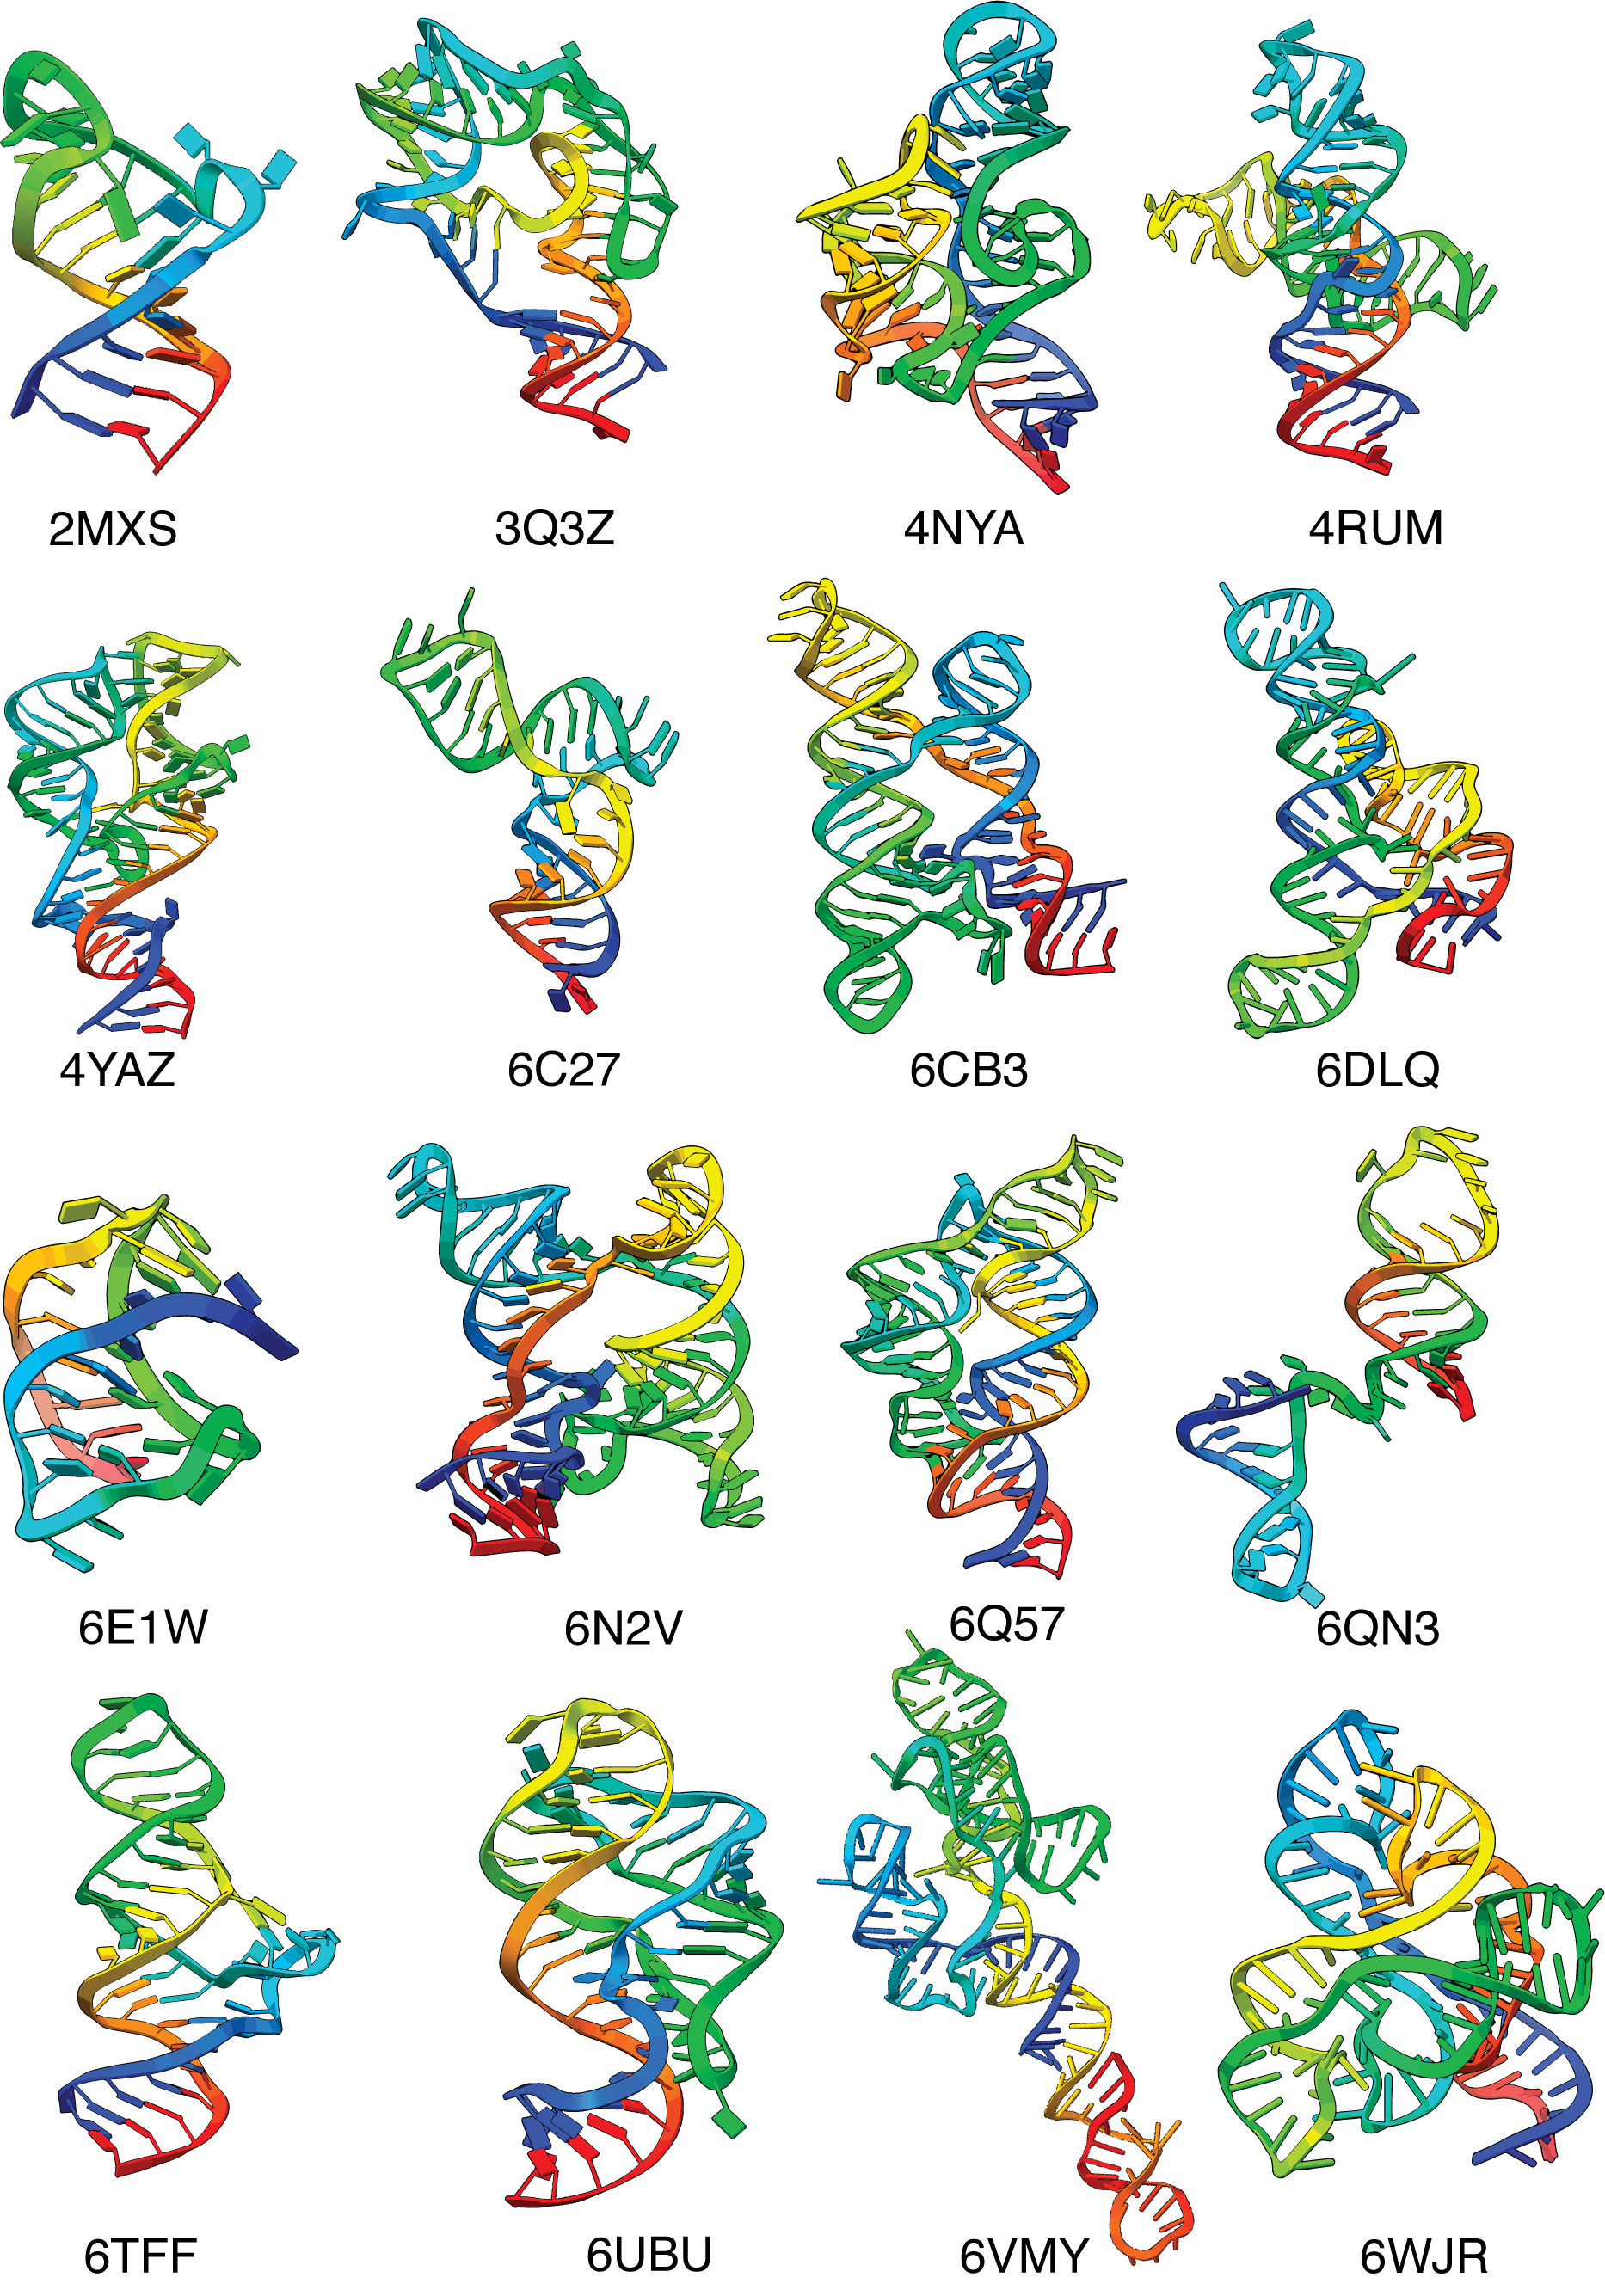
\includegraphics[
    width=\textwidth
    ]{./all-representatives.png}
    \caption{{\bf Riboswitch reference conformations labeled with PDB accession code.}}
    \label{fig:all-representatives}%
\end{figure*}

\begin{figure}
    \centering
    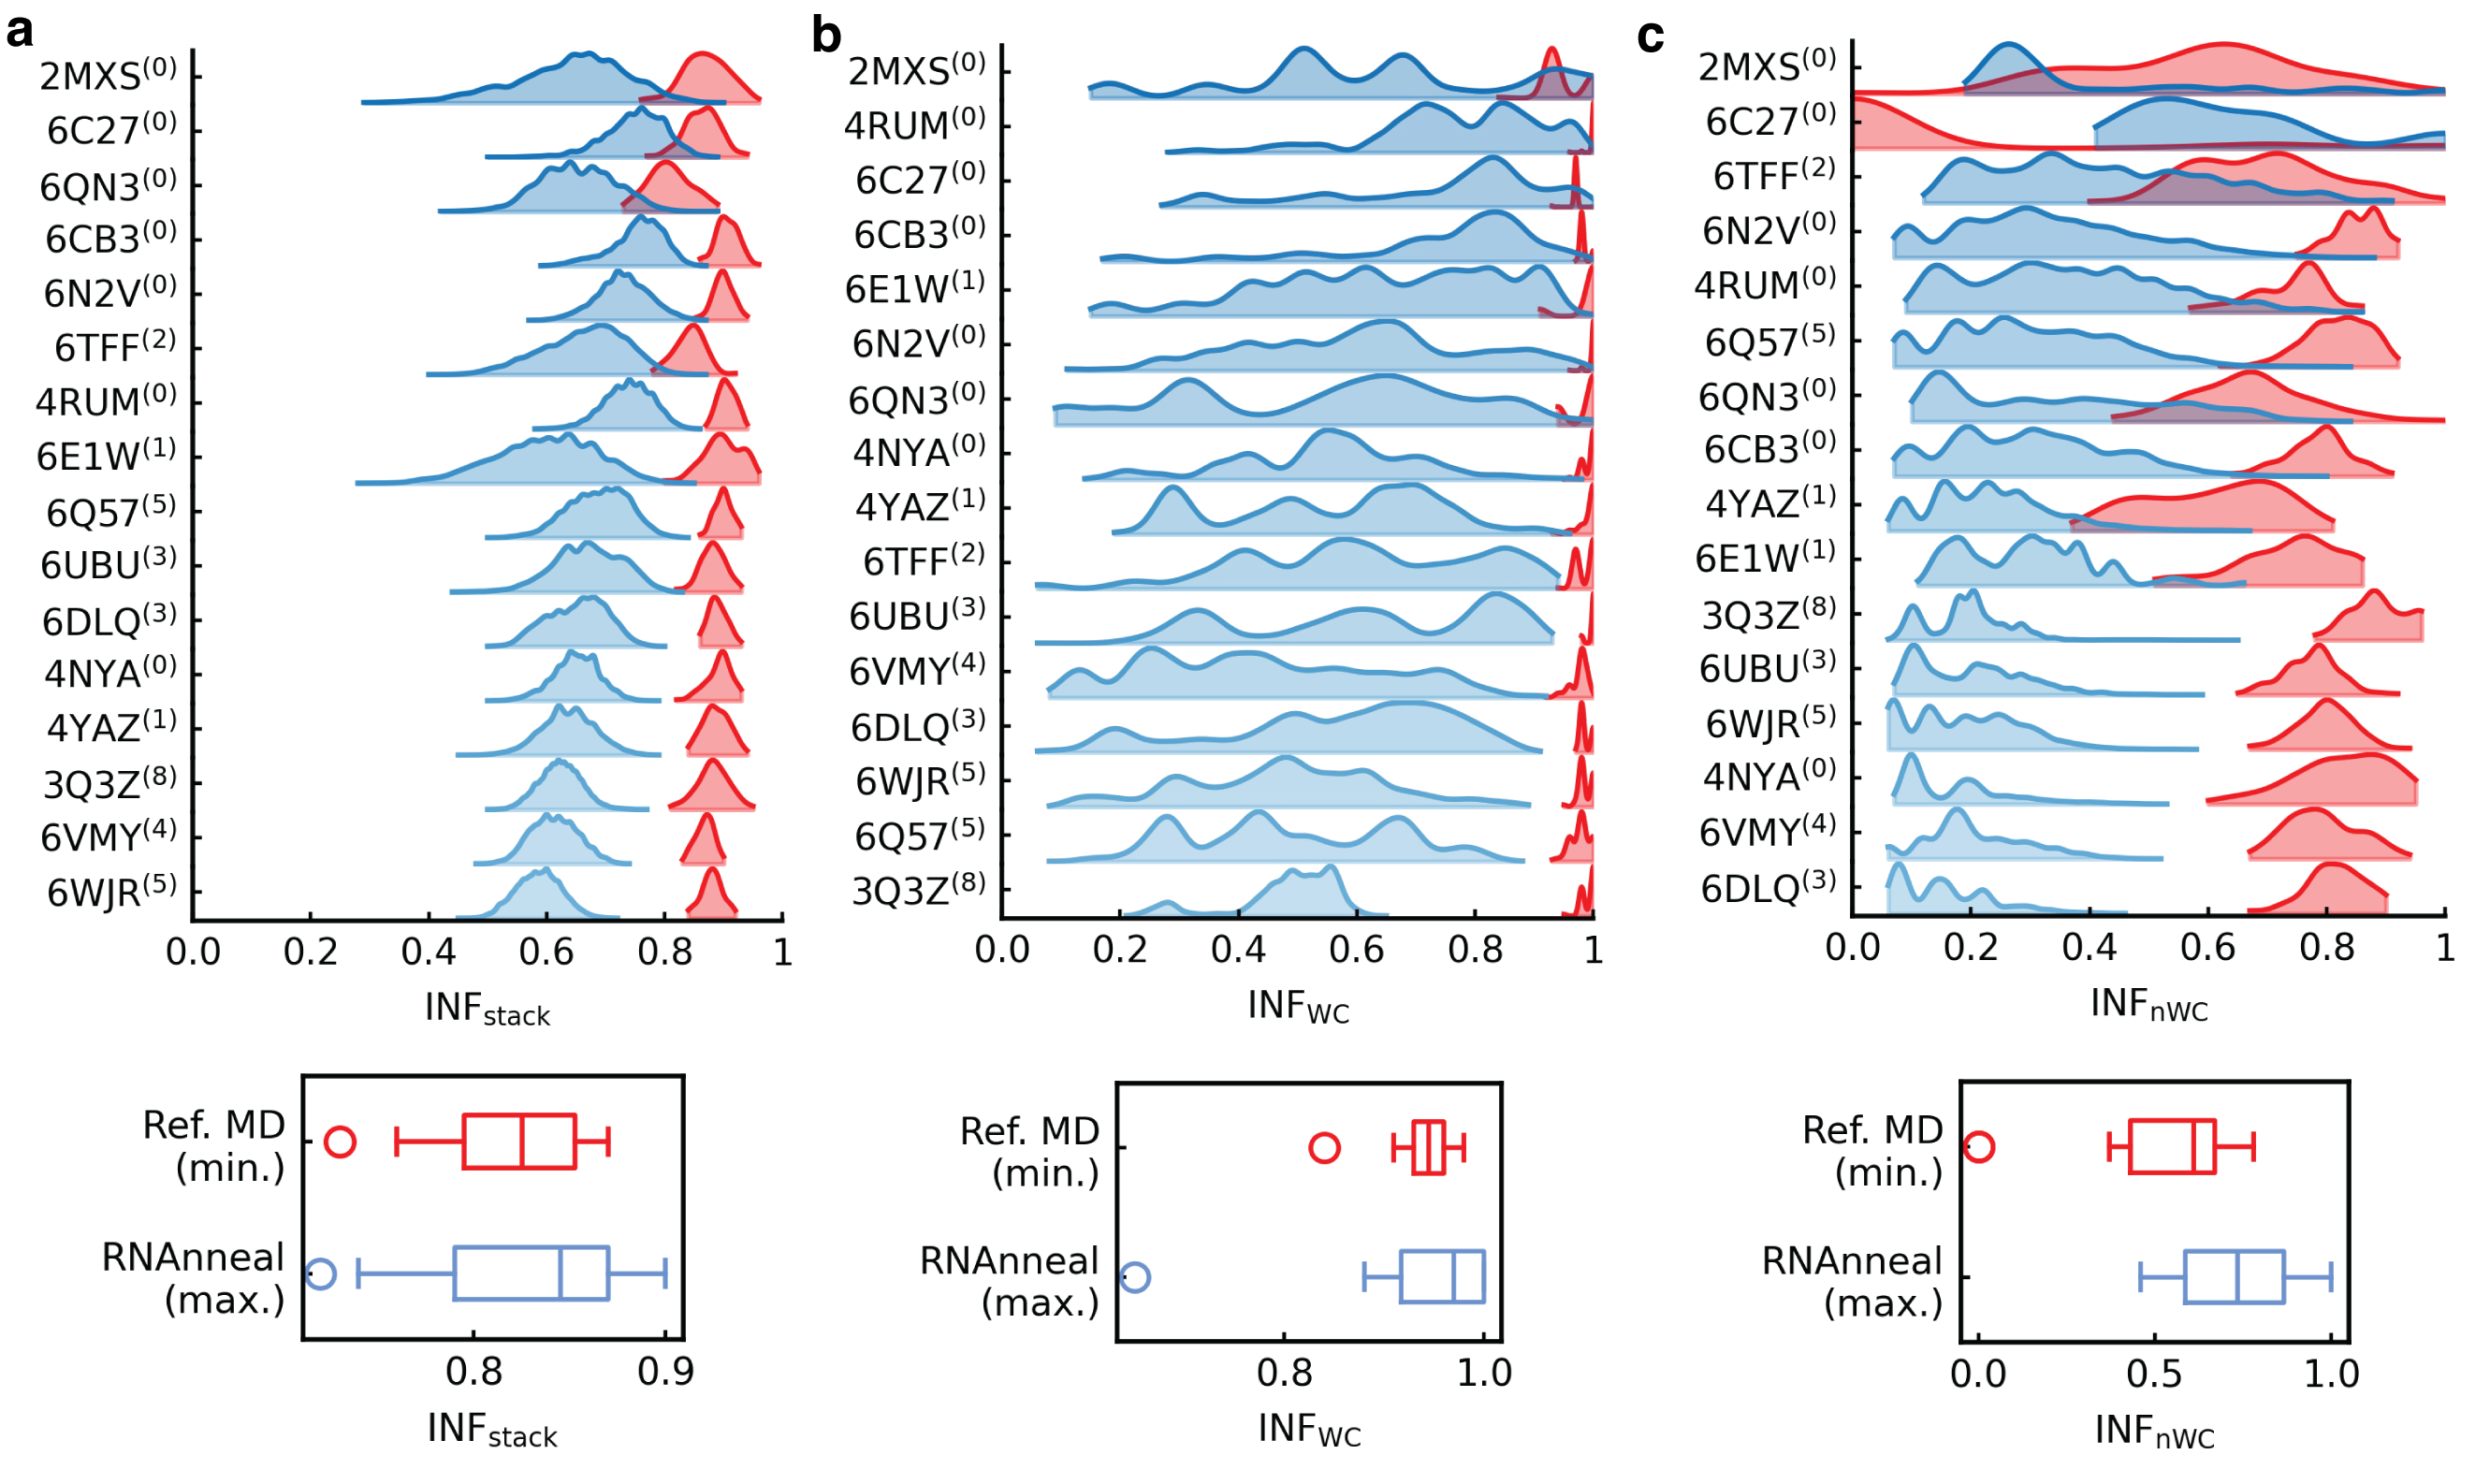
\includegraphics[
    width=0.9\textwidth
    ]{./stack-wc-nwc.png}
    \caption{{\bf Interaction Network Fidelity (INF) by interaction type.} The INF is reported for {\textbf{a}.} stacking interactions (Median [IQR]; Ref. MD: 0.82 [$0.79-0.86$]; RNAnneal: 0.85 [$0.80-0.87$]),  {\textbf{b}.} Watson-Crick (WC) interactions (Ref. MD: 0.95 [$0.93-0.96$]; RNAnneal: 0.98 [$0.92-1.0$]), {\textbf{c}.} non-Watson-Crick (nWC) interactions (Ref. MD: 0.62 [$0.48-0.67$]; RNAnneal: 0.80 [$0.59-0.87$]). It is worth noting that the conformation with, e.g., the maximum $\mathrm{INF_{WC}}$, does not necessarily have the maximum $\mathrm{INF_{stack}}$ or $\mathrm{INF_{nWC}}$.}
    \label{fig:inf-detailed}%
\end{figure}

\begin{figure}
    \centering
    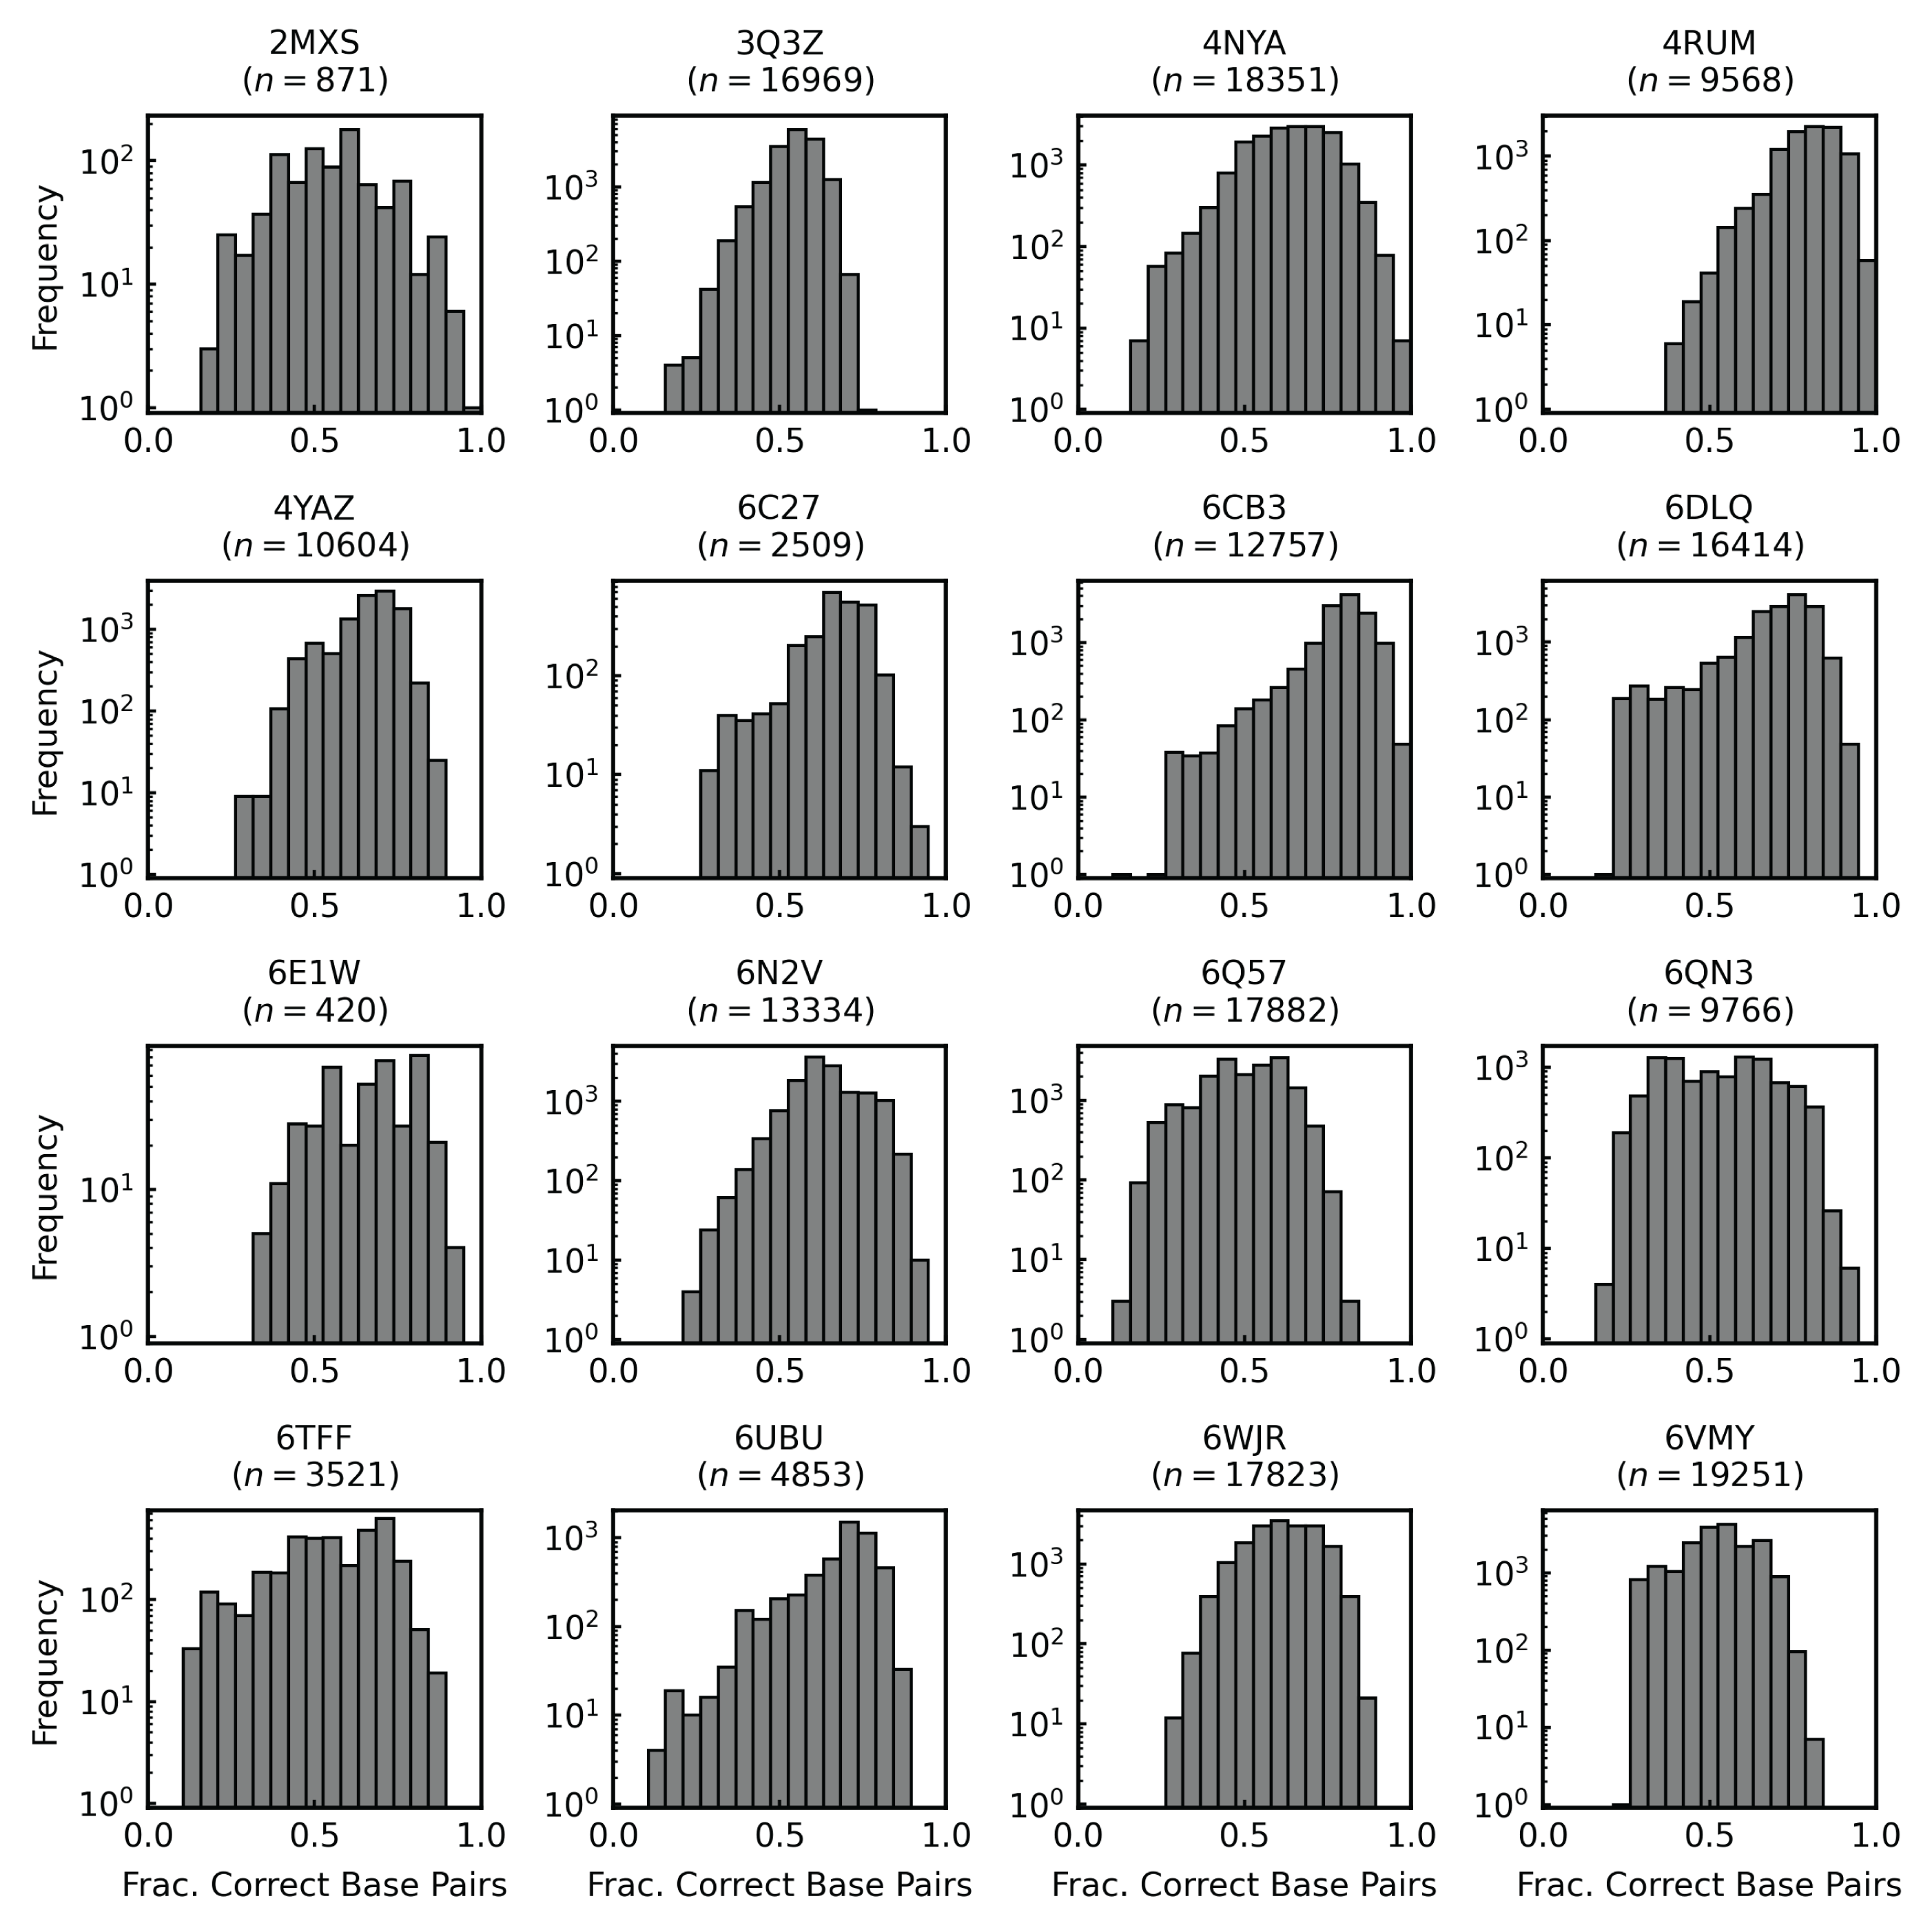
\includegraphics[
    width=0.9\textwidth
    ]{./sec-struct-all.png}
    \caption{{\bf Evaluation of secondary structures predicted by EternaFold, LinearFold, and LinearAlifold.} Secondary structures sampled by Eternafold, LinearFold, and LinearAilfold are compared to the reference secondary structure extracted from the listed PDB entry; $n$ denotes the total number of secondary structures sampled.}
    \label{fig:sec-struct-eval}%
\end{figure}

\begin{figure}
    \centering
    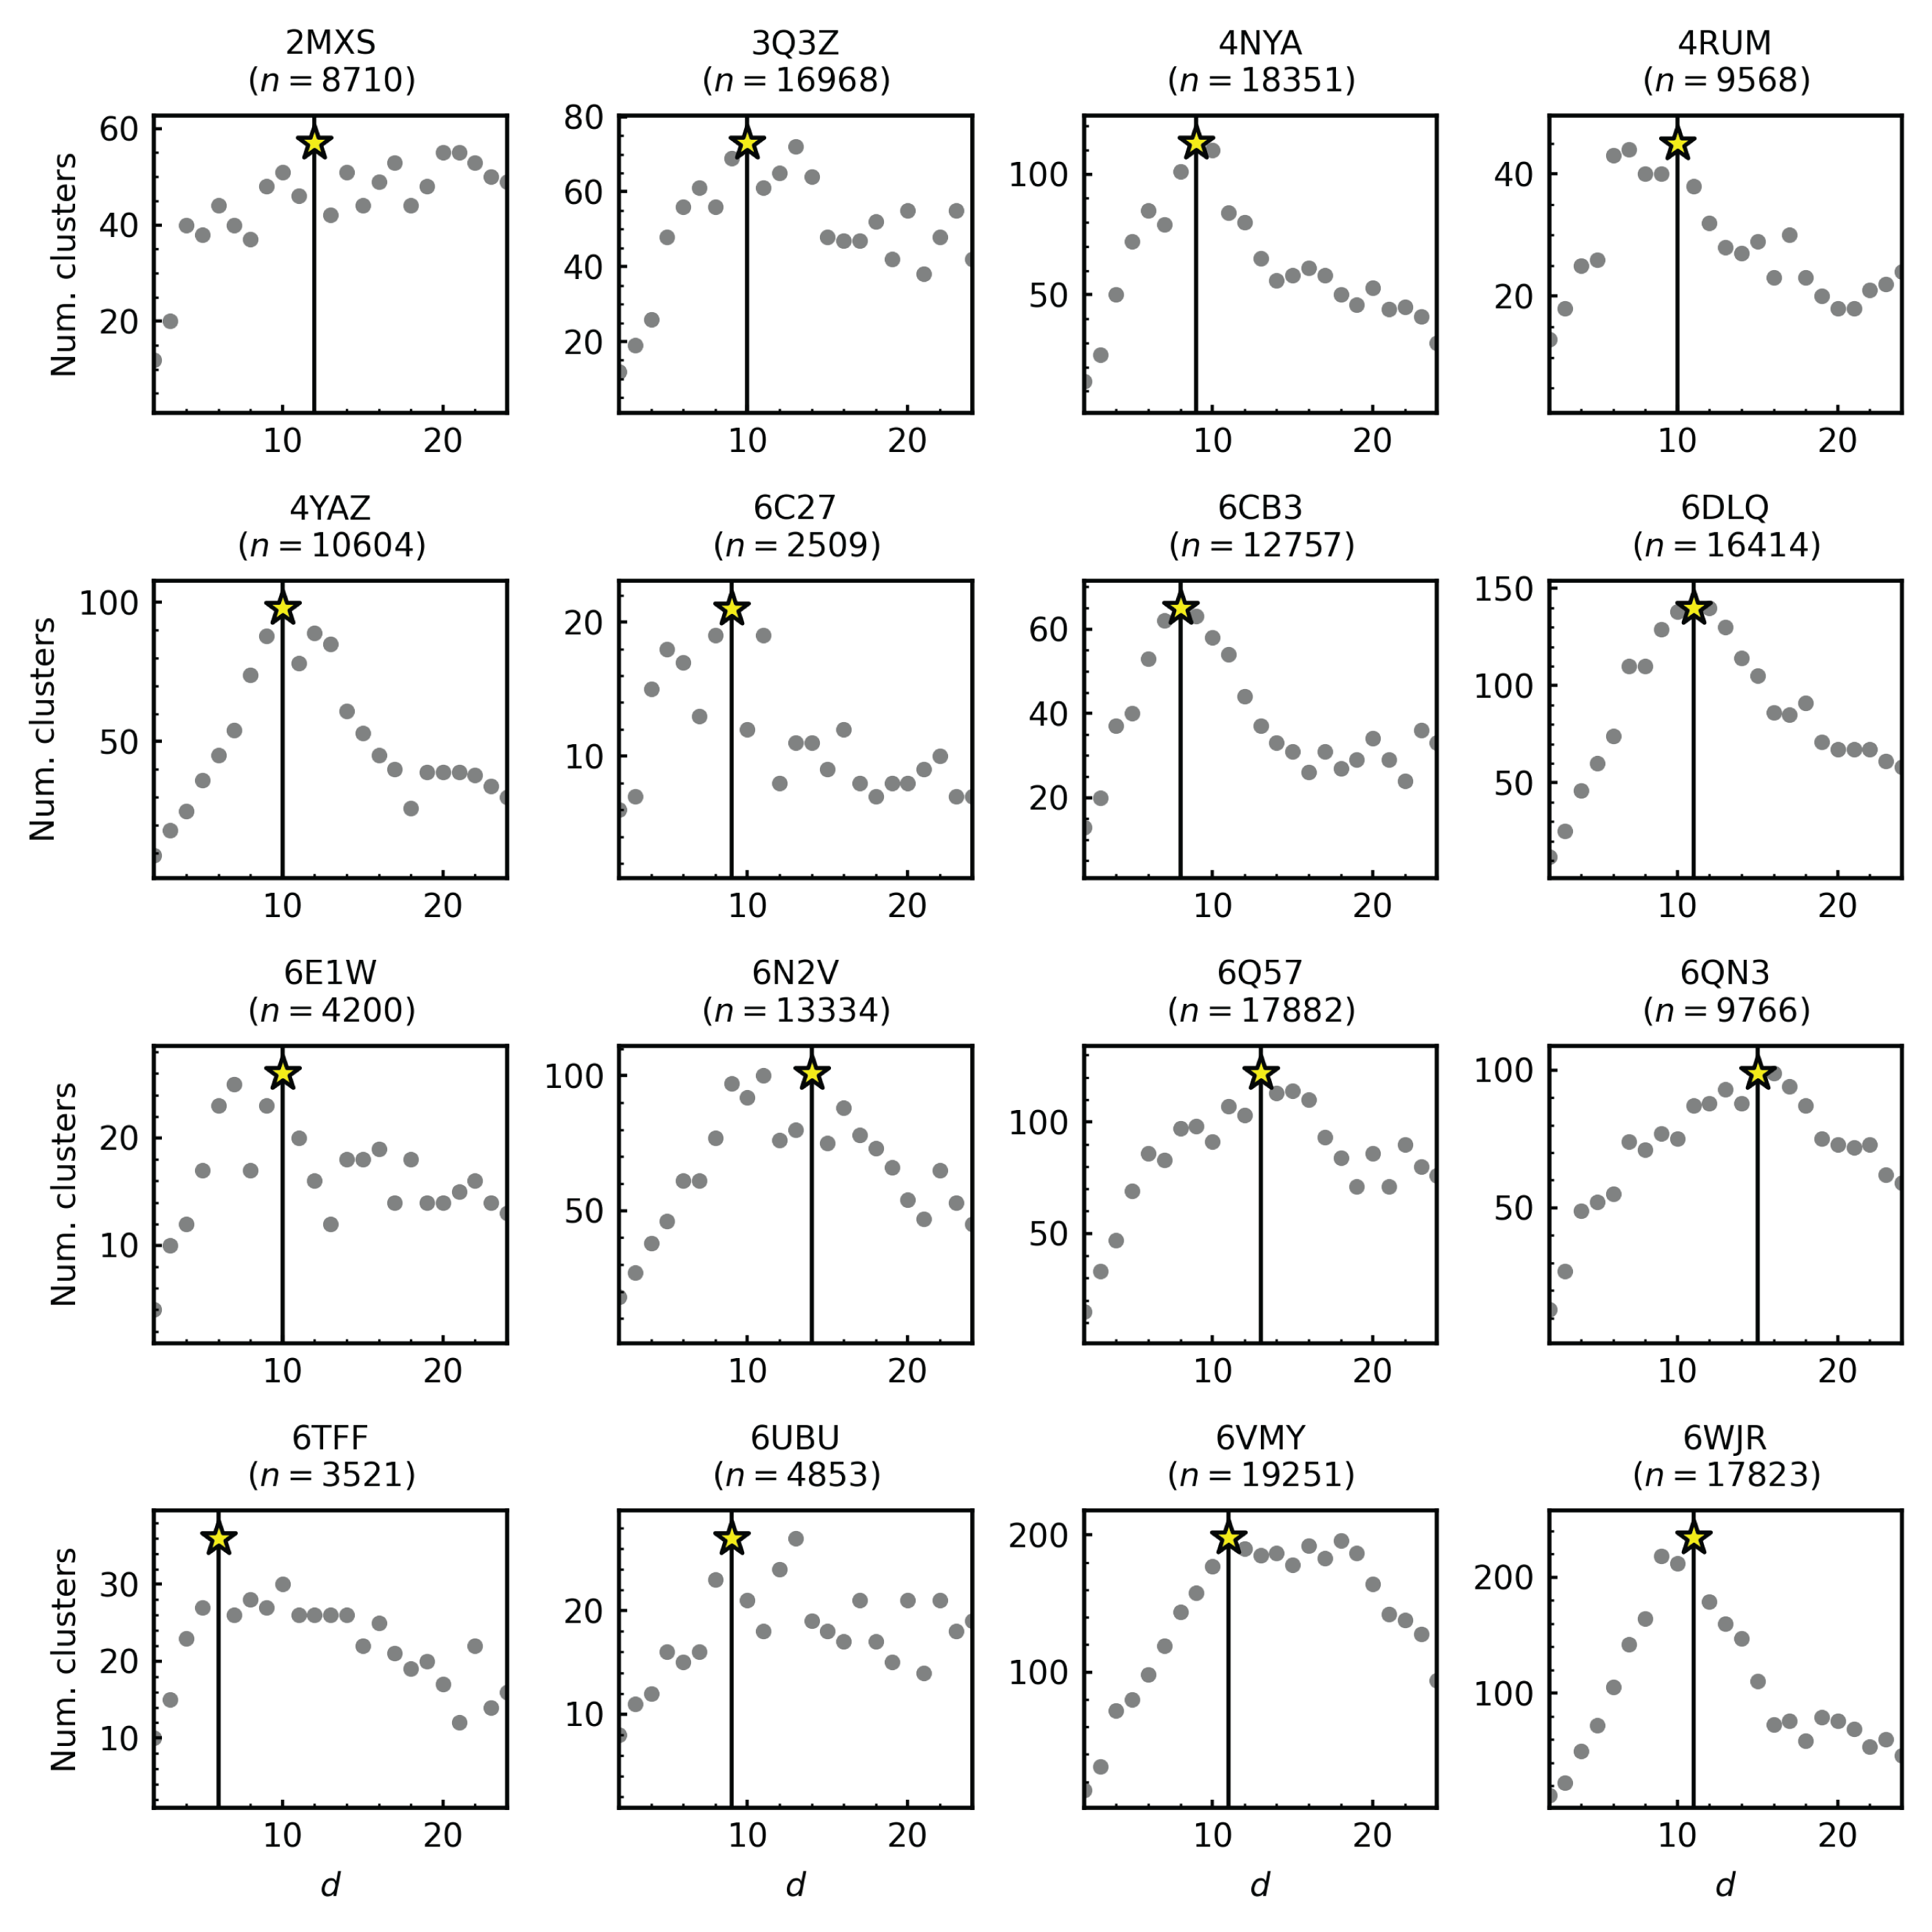
\includegraphics[
    width=0.9\textwidth
    ]{./clusters_vs_d.png}
    \caption{{\bf Number of clusters vs d.} For each RNA, the G-vectors are projected onto $d$ components, and clustering is performed via the Advanced Density Peaks algorithm implemented in \texttt{dadapy}. The number of clusters, $N_c$ is recorded as a function of $d$. The star values and vertical line indicate the $d$ where $N_c$ is maximized; $n$ denotes the total number of tertiary models used in the calculation.}
    \label{fig:clusters_vs_d}%
\end{figure}



\begin{figure}
    \centering
    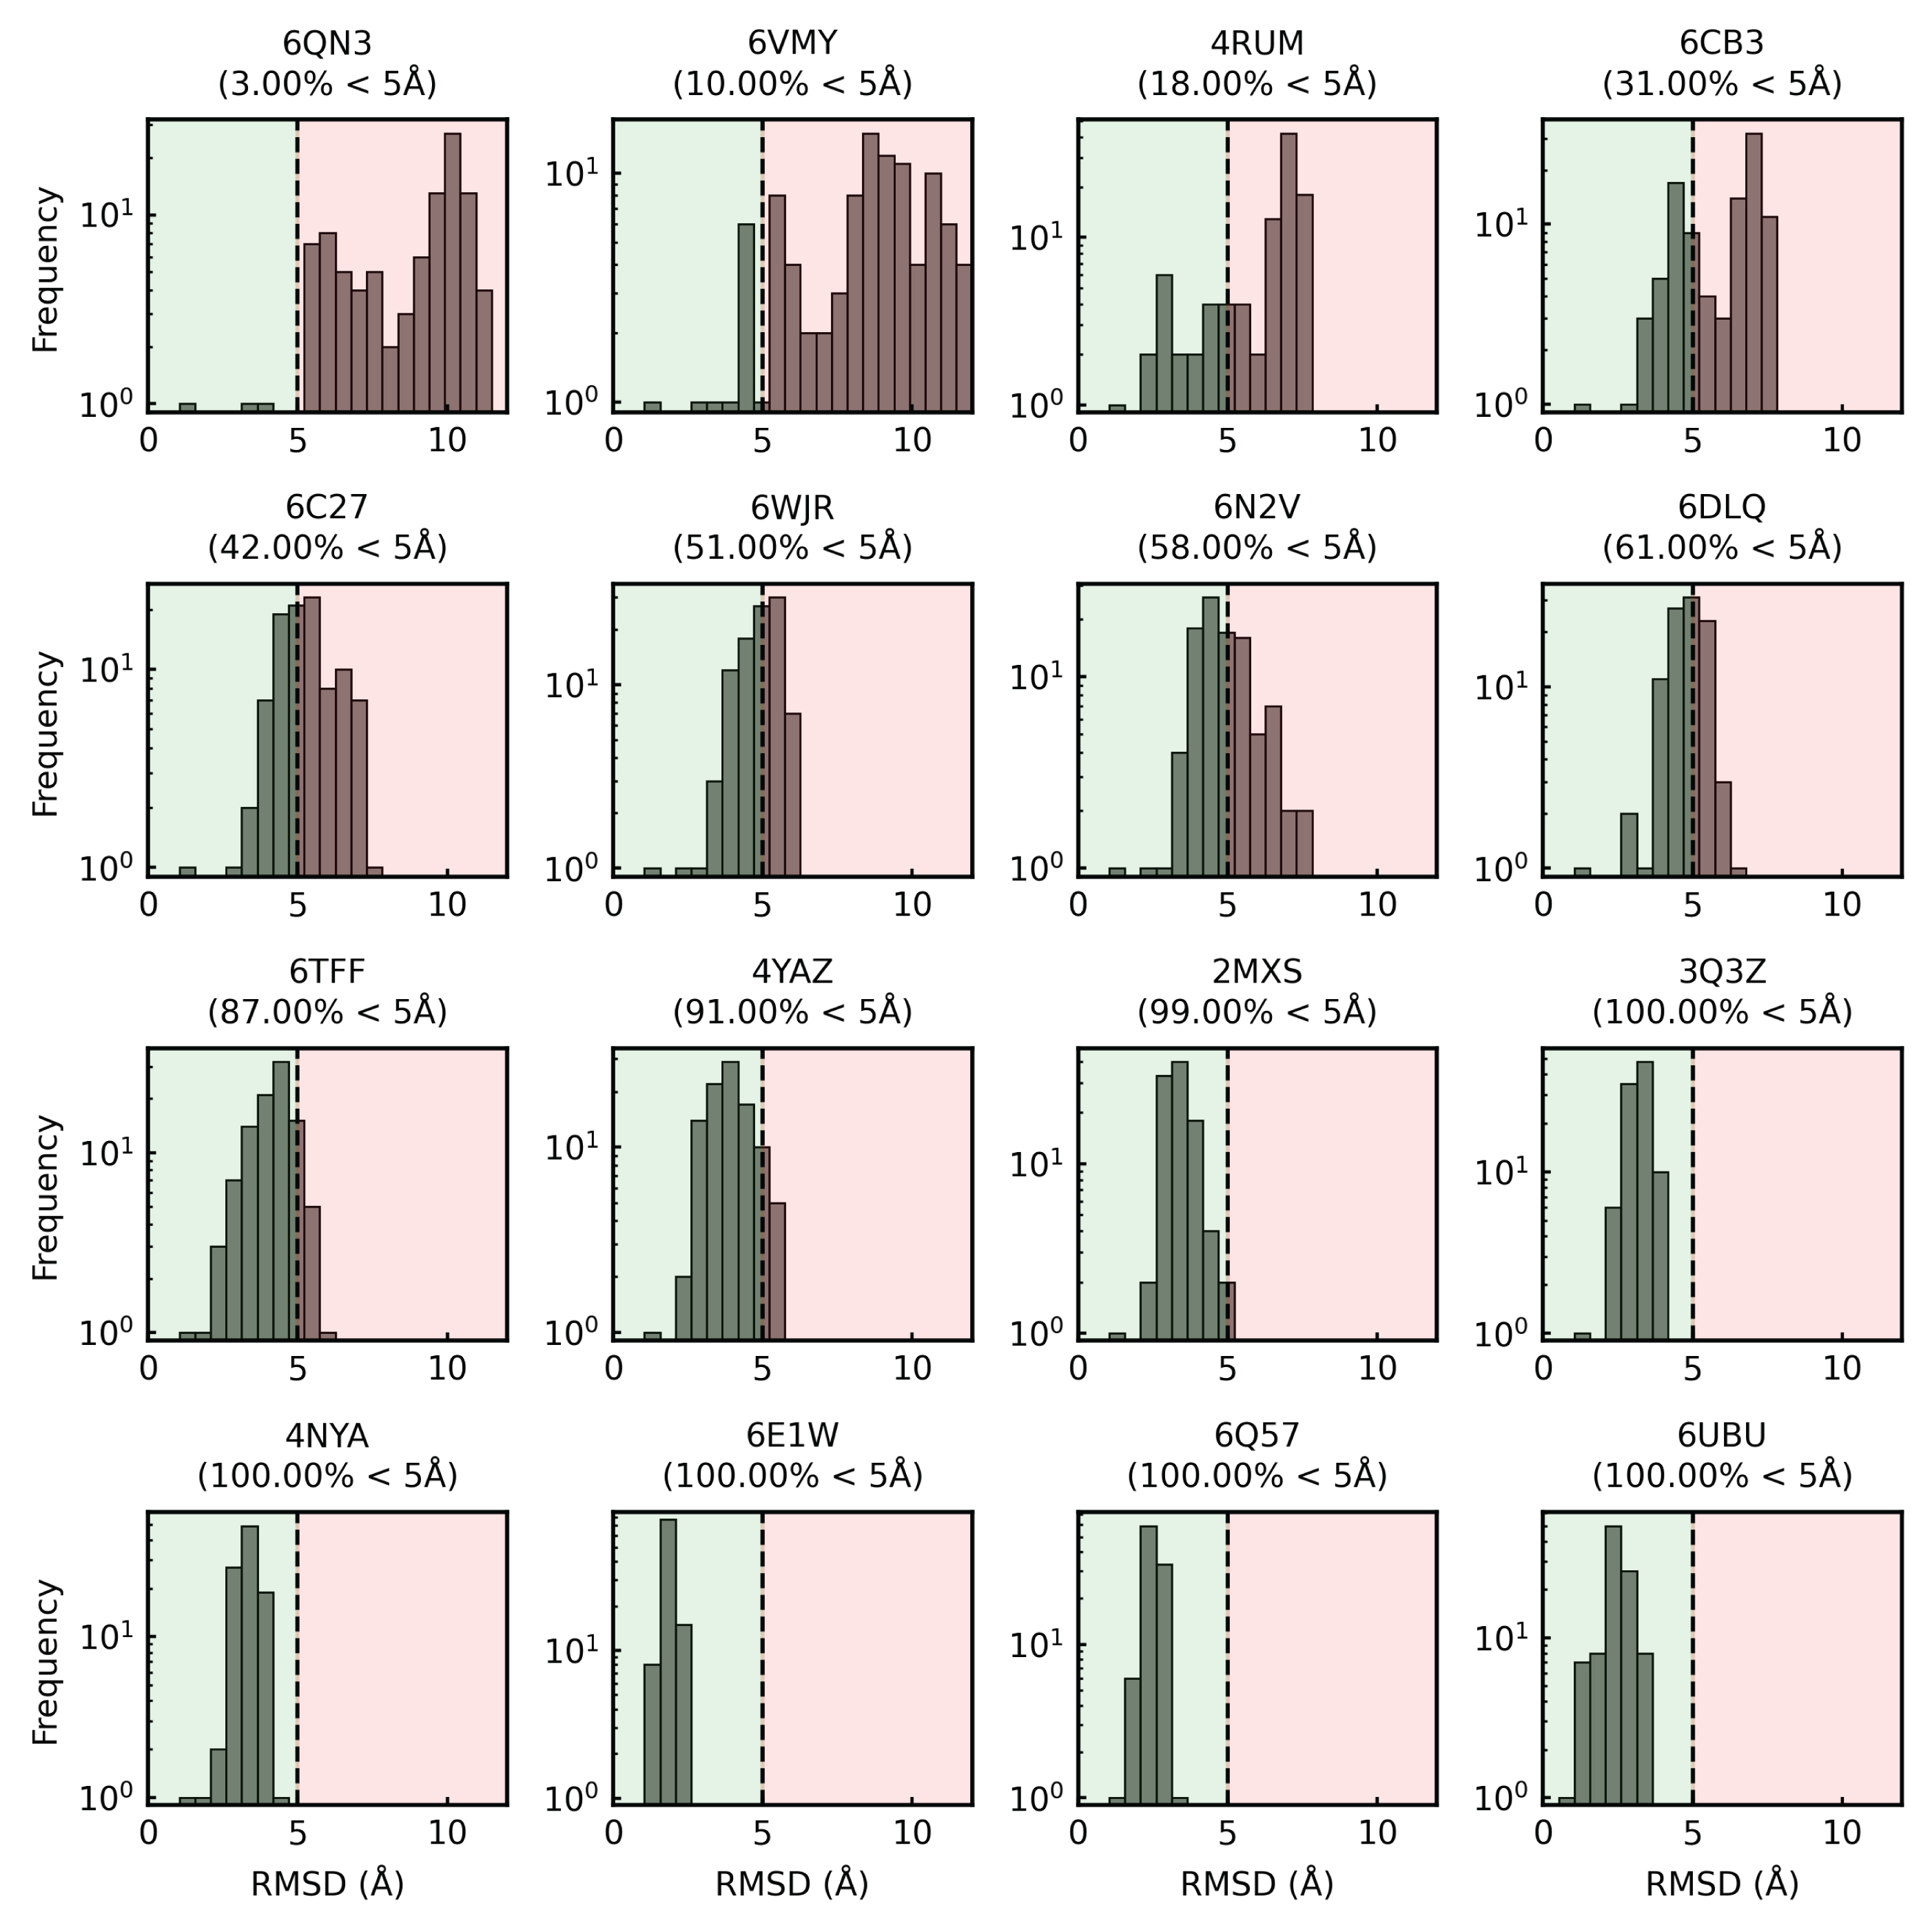
\includegraphics[
    width=0.9\textwidth
    ]{./rmsd_reference.png}
    \caption{{\bf RMSD variation over a 100ns MD simulation launched from the reference conformation.} The dashed line placed at $5${\AA} indicates the cutoff used to classify ``realistic'' (RMSD$\leq5${\AA}) and ``decoy''(RMSD$>5${\AA}) conformations. The proportion of realistic conformations is provided underneath the PDB accession code.}
    \label{fig:rmsd_reference}%
\end{figure}

\begin{figure}
    \centering
    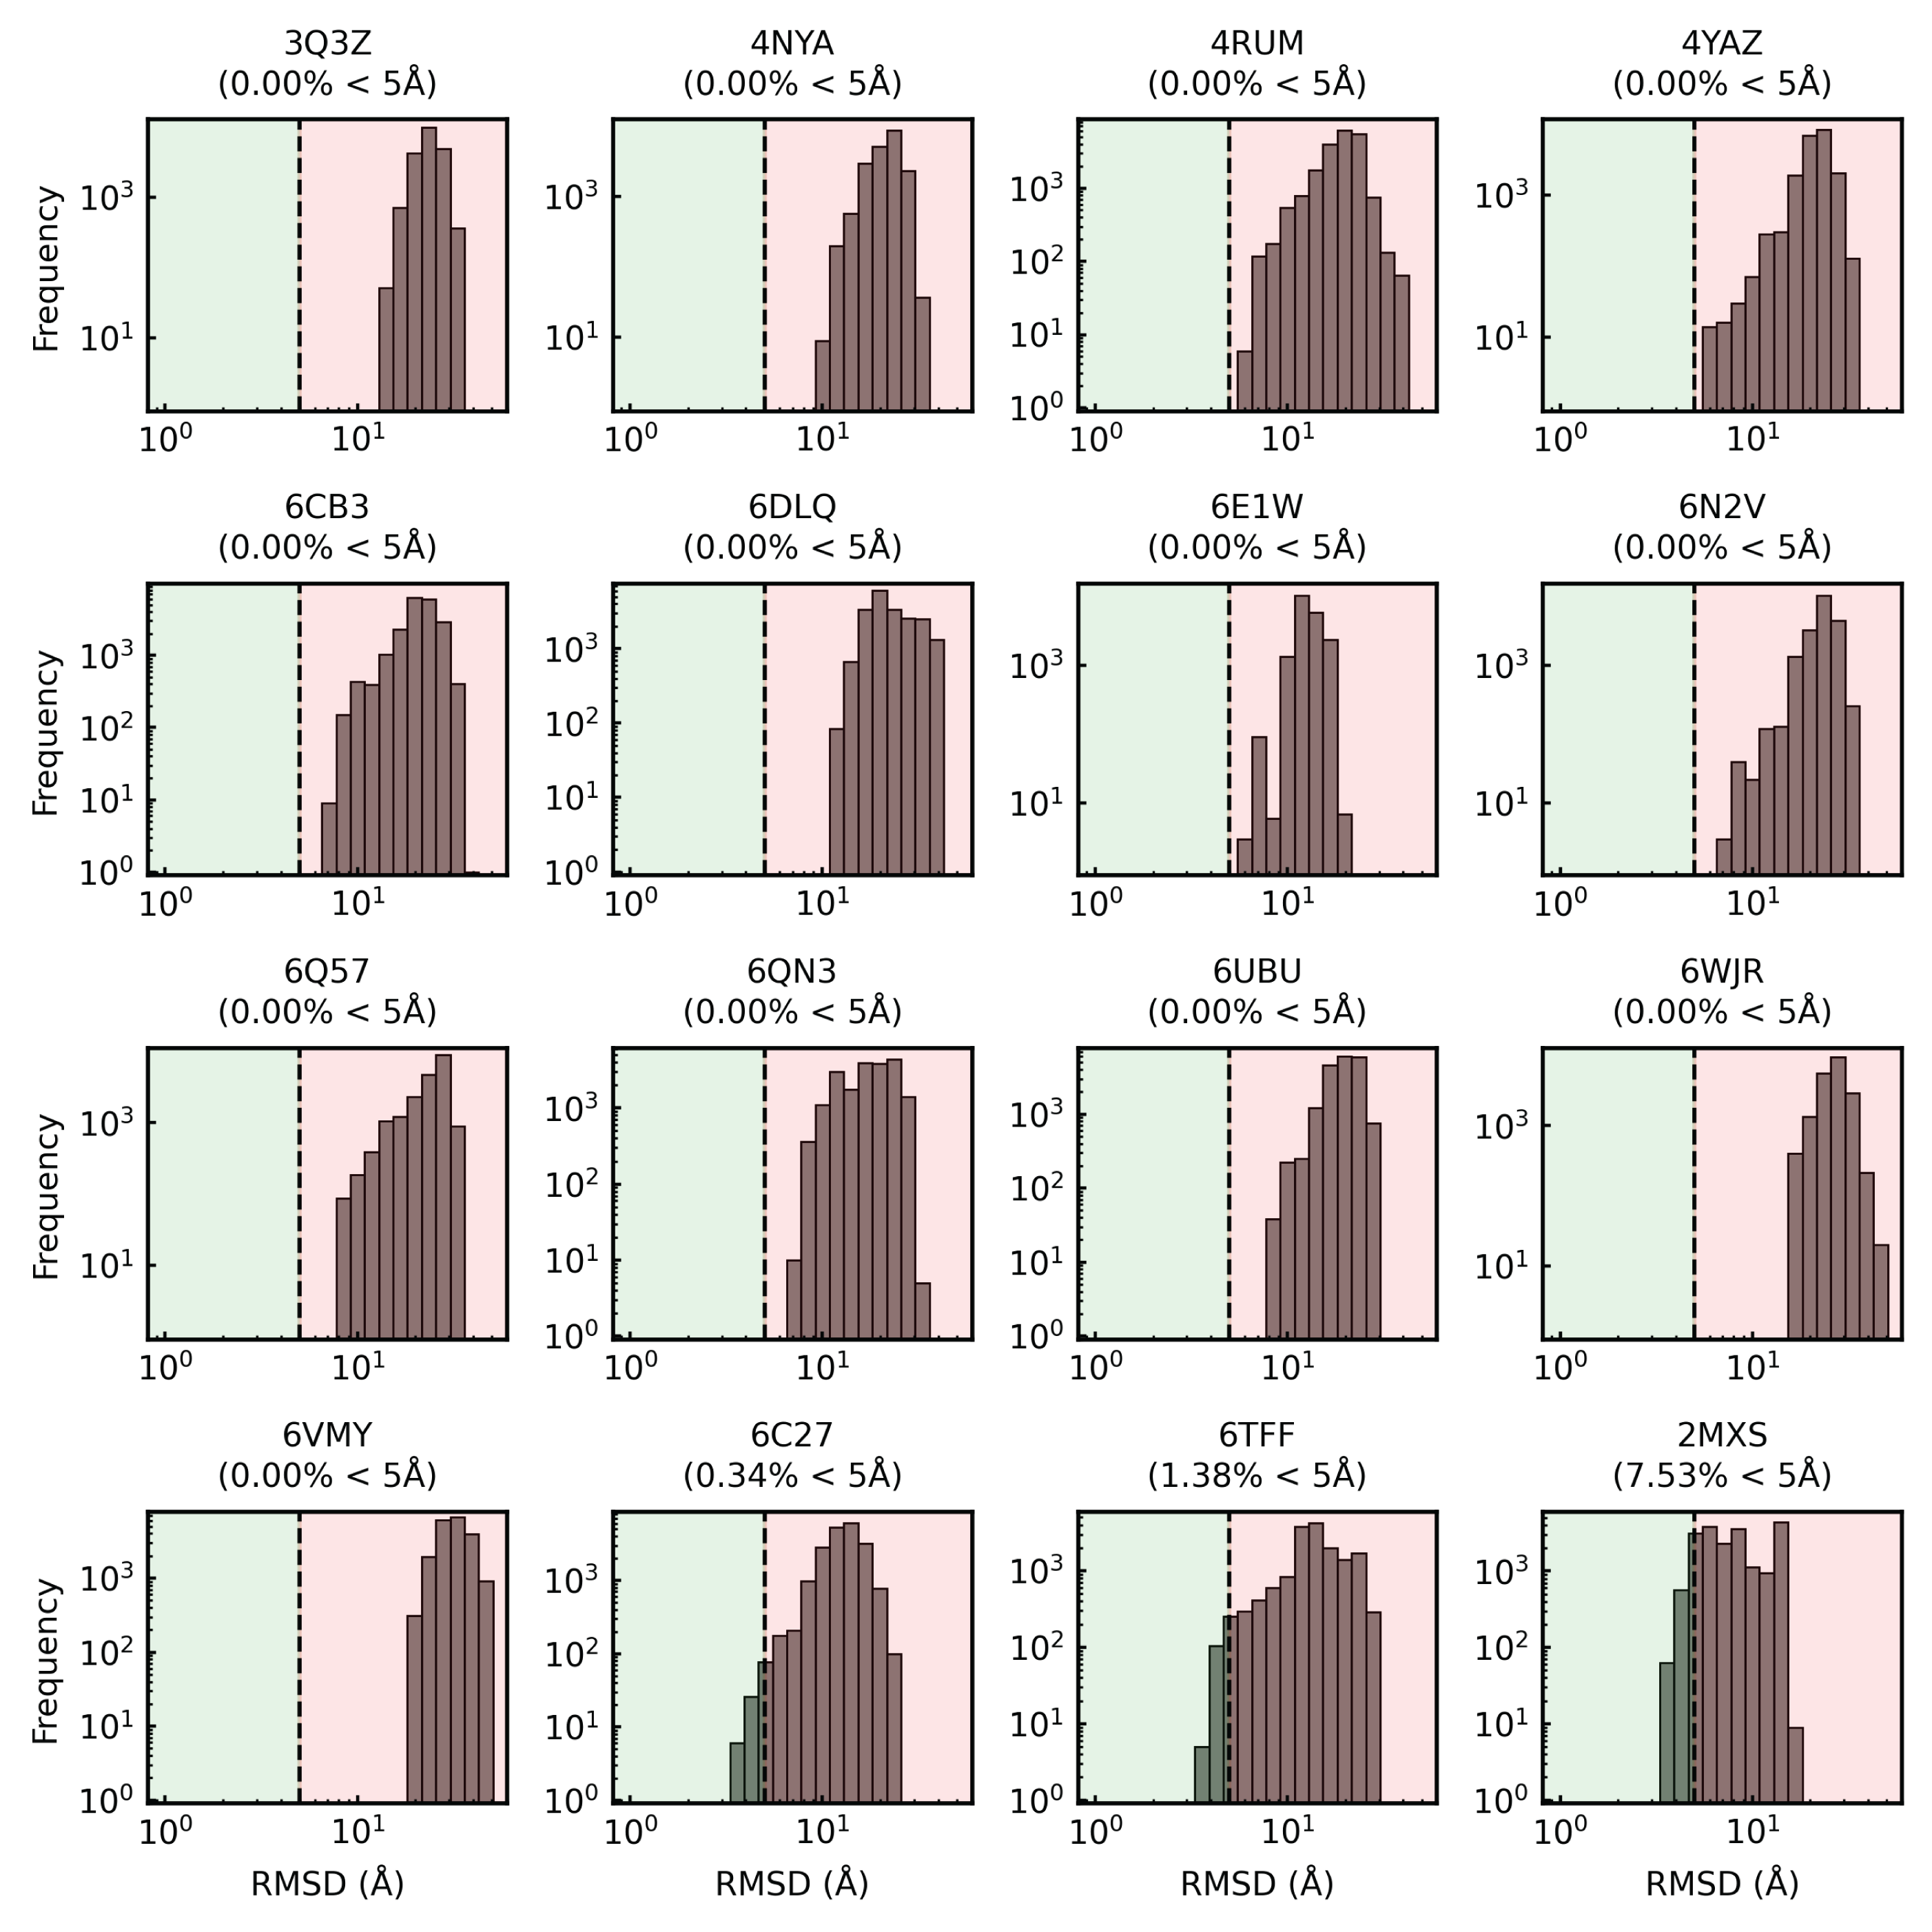
\includegraphics[
    width=0.9\textwidth
    ]{./rmsd_decoys.png}
    \caption{{\bf RMSD distribution of conformations sampled by RNAnneal.} The dashed line placed at $5${\AA} indicates the cutoff used to classify ``realistic'' (RMSD$\leq5${\AA}) and ``decoy'' (RMSD$>5${\AA}) conformations. The proportion of realistic conformations is provided underneath the PDB accession code.}
    \label{fig:rmsd_decoys}%
\end{figure}

\begin{figure}
    \centering
    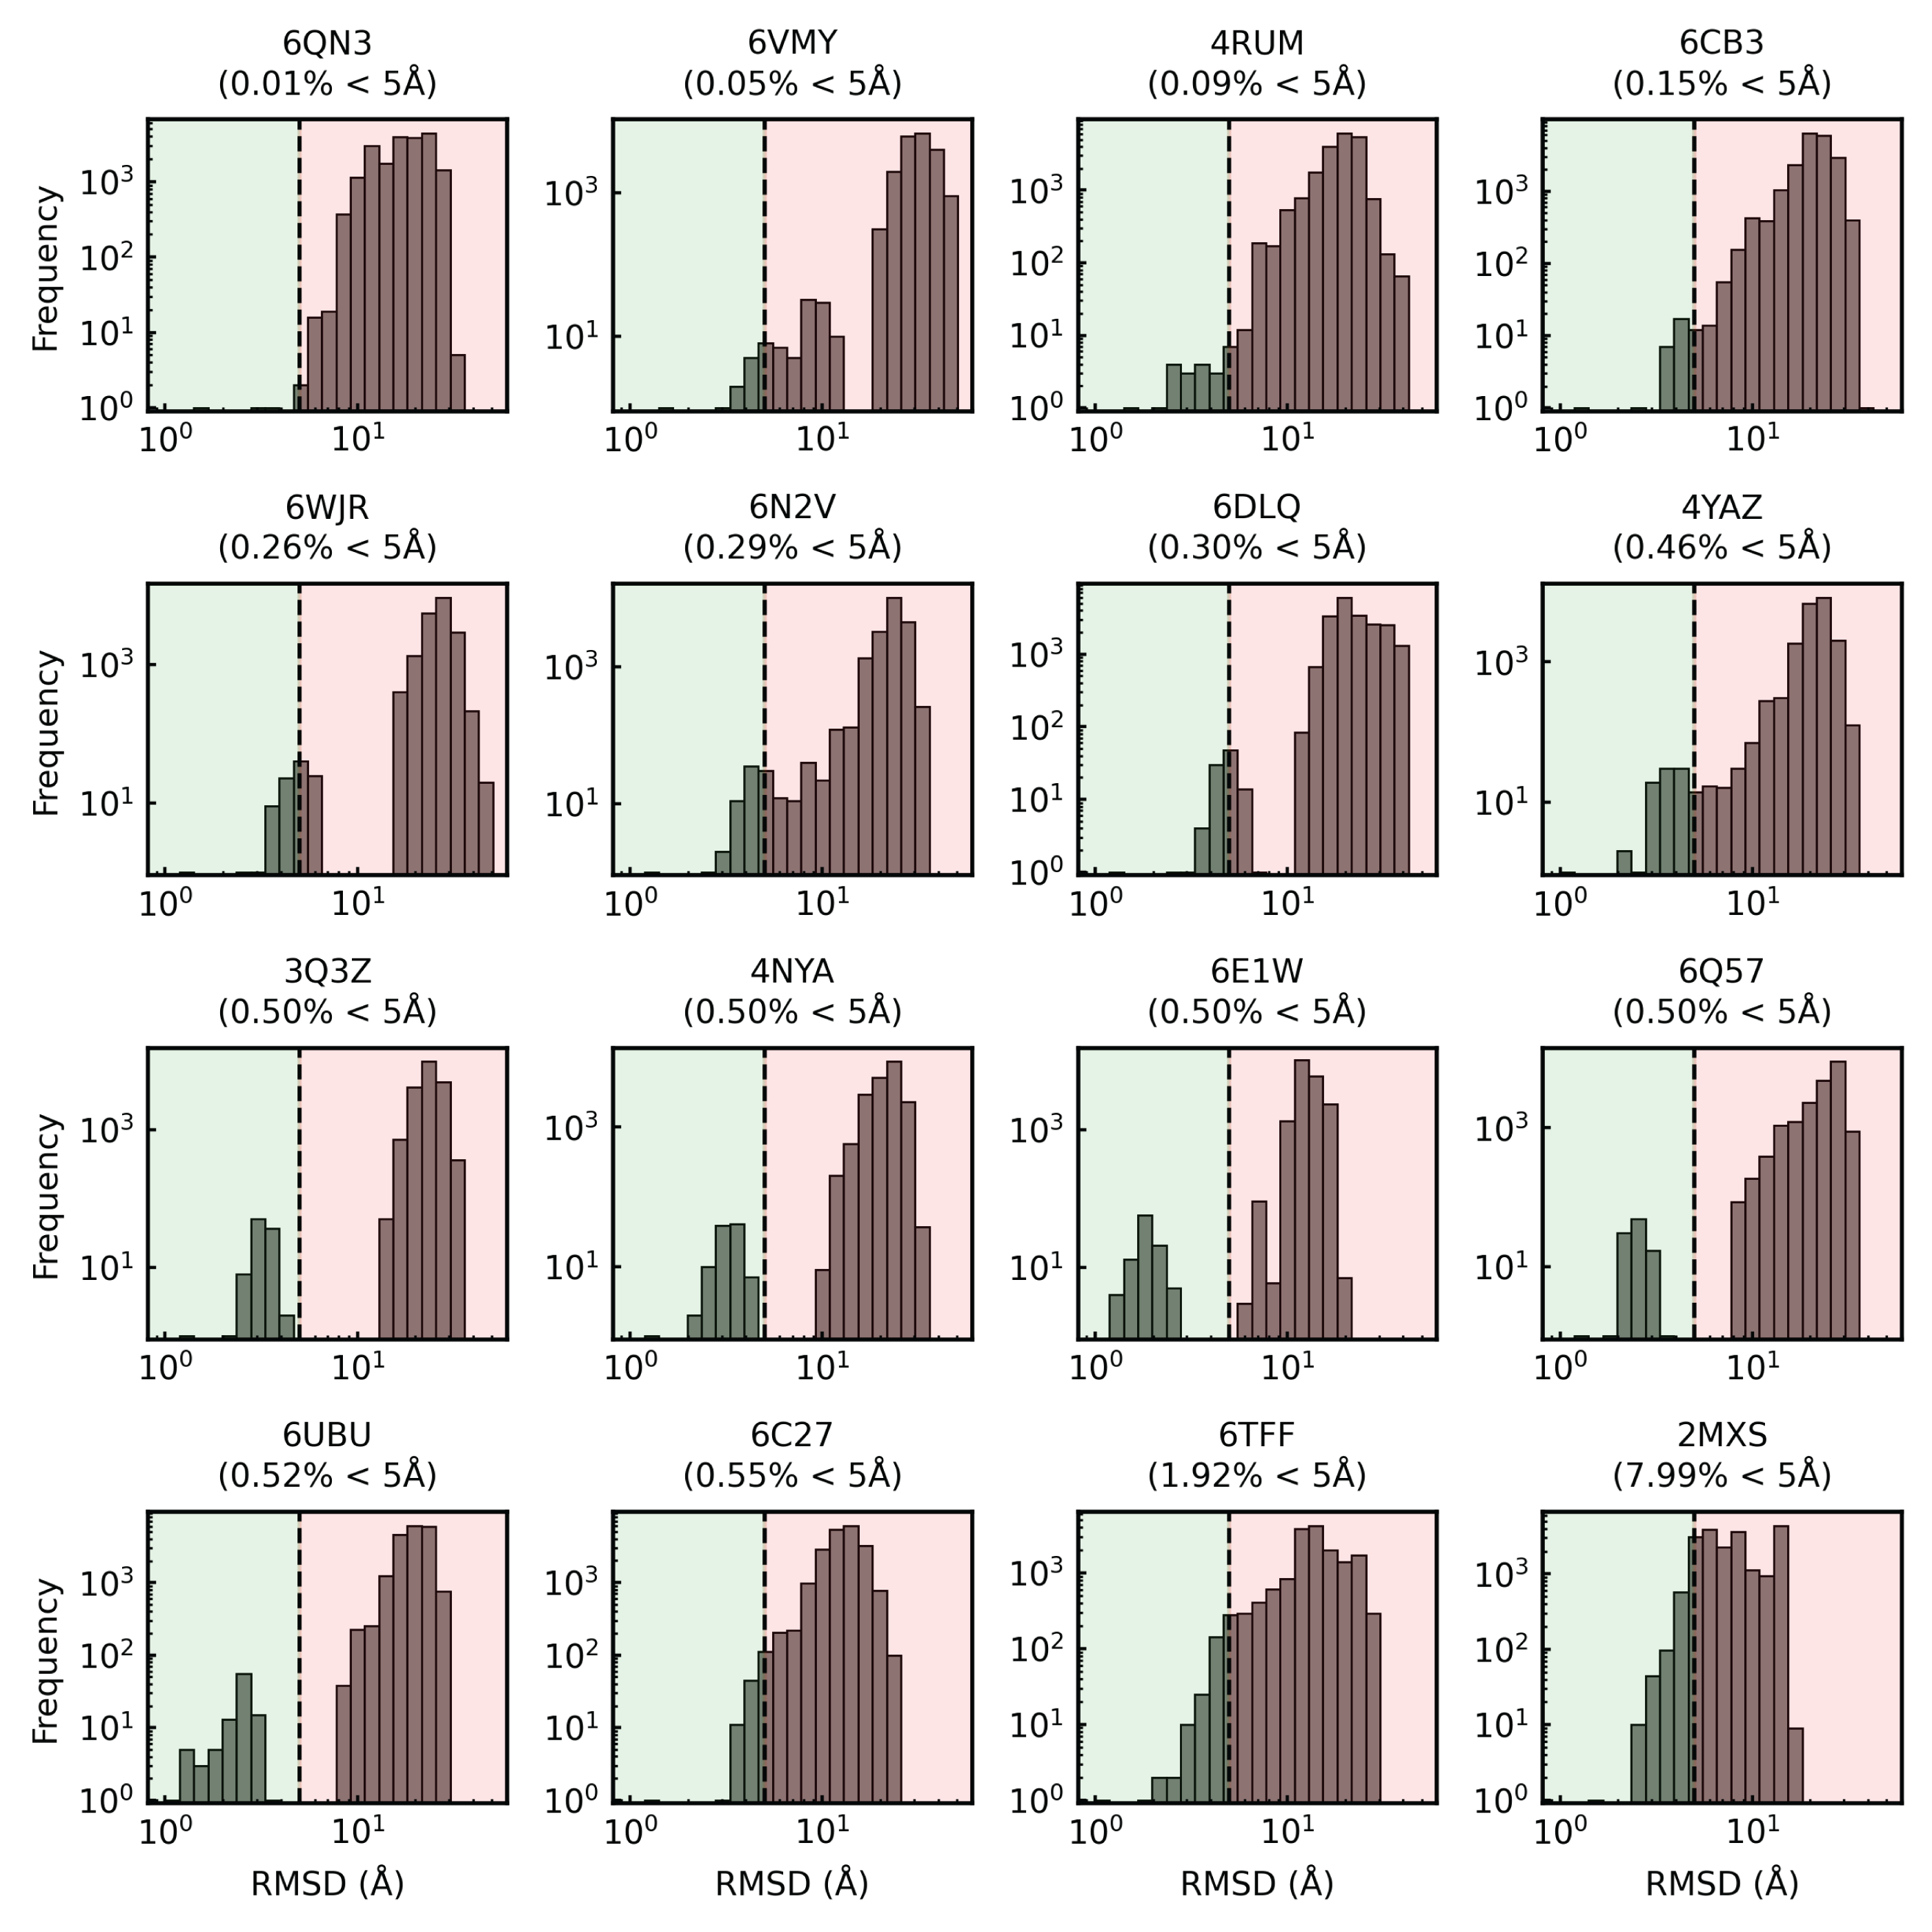
\includegraphics[
    width=0.9\textwidth
    ]{./rmsd_combined.png}
    \caption{{\bf RMSD distribution of conformations for the classification task.} The classification task merges structures sampled by RNAnneal with frames from simulations launched from the reference conformations (i.e., merges Fig. S\ref{fig:rmsd_reference} and S\ref{fig:rmsd_decoys}). The dashed line placed at $5${\AA} indicates the cutoff used to classify ``realistic'' (RMSD$\leq5${\AA}) and ``decoy'' (RMSD$>5${\AA}) conformations. The proportion of realistic conformations is provided underneath the PDB accession code.}
    \label{fig:rmsd_combined}%
\end{figure}

\begin{figure}
    \centering
    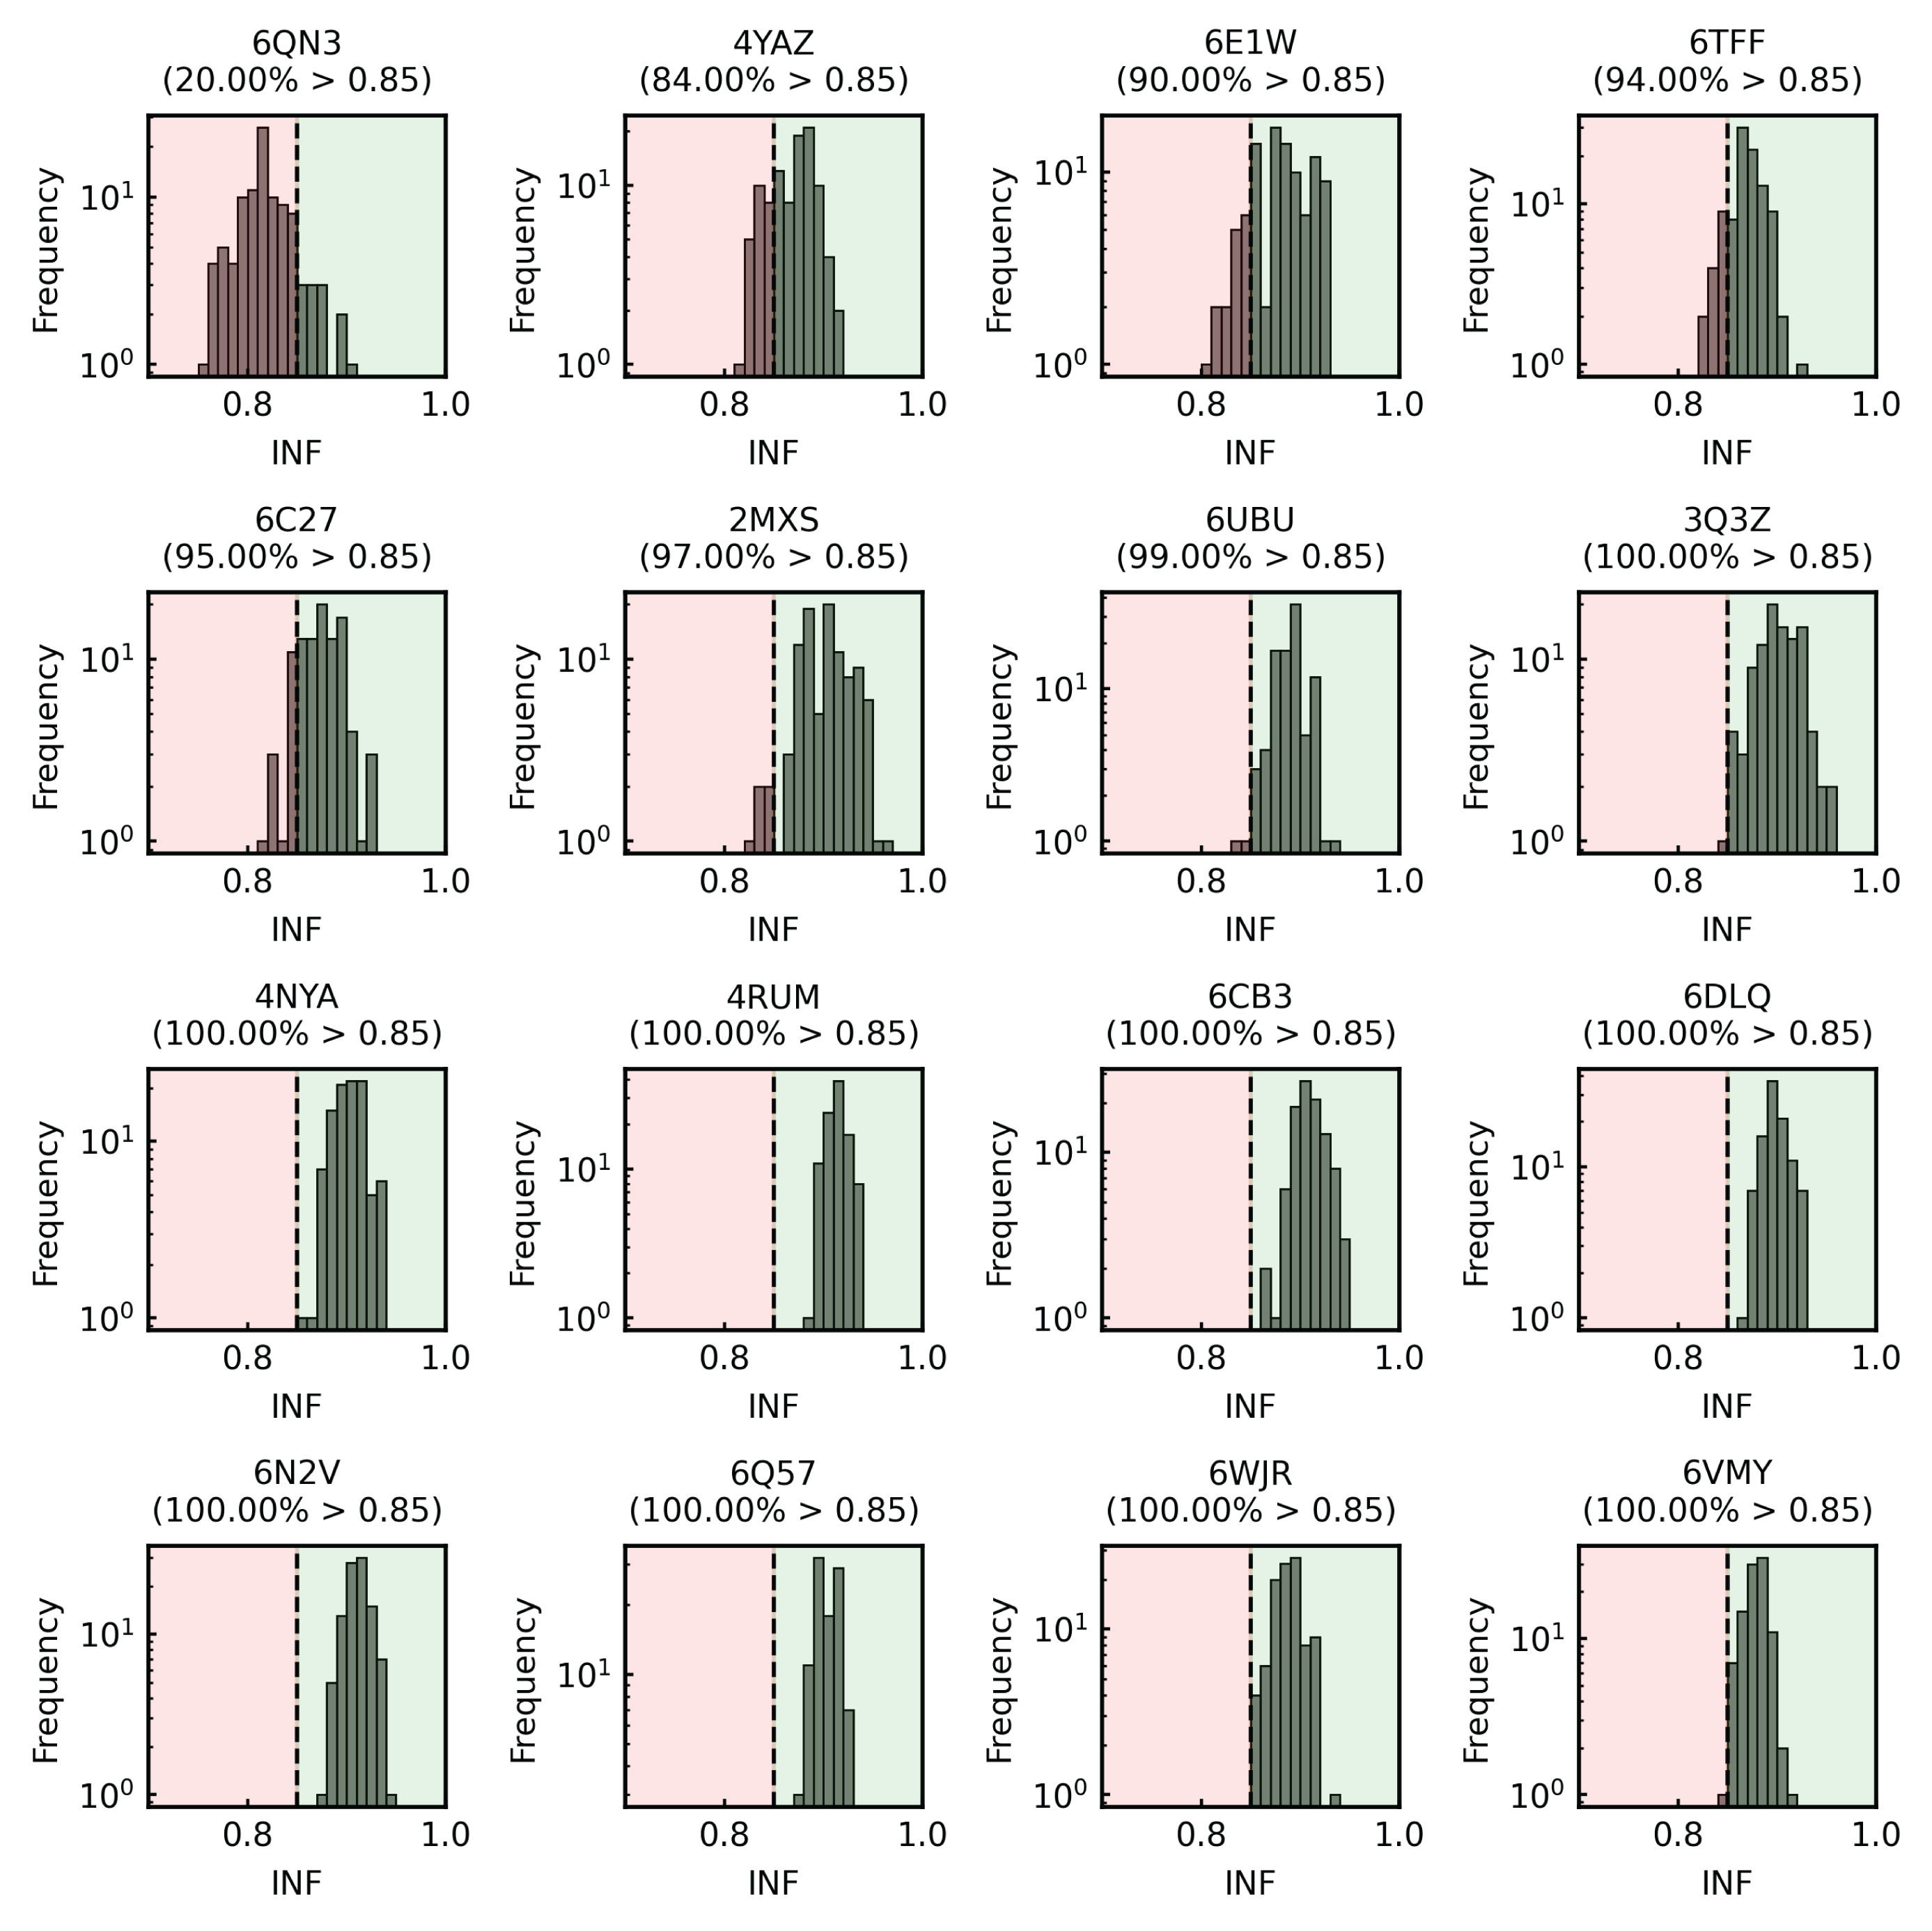
\includegraphics[
    width=0.9\textwidth
    ]{./inf_reference.png}
    \caption{{\bf INF variation over a 100ns MD simulation launched from the reference conformation.} The dashed line placed at $0.85$ indicates the cutoff used to classify ``realistic'' (INF$\geq$0.85) and ``decoy'' (INF$<$0.85) conformations. The proportion of realistic conformations is provided underneath the PDB accession code.}
    \label{fig:inf_reference}%
\end{figure}

\begin{figure}
    \centering
    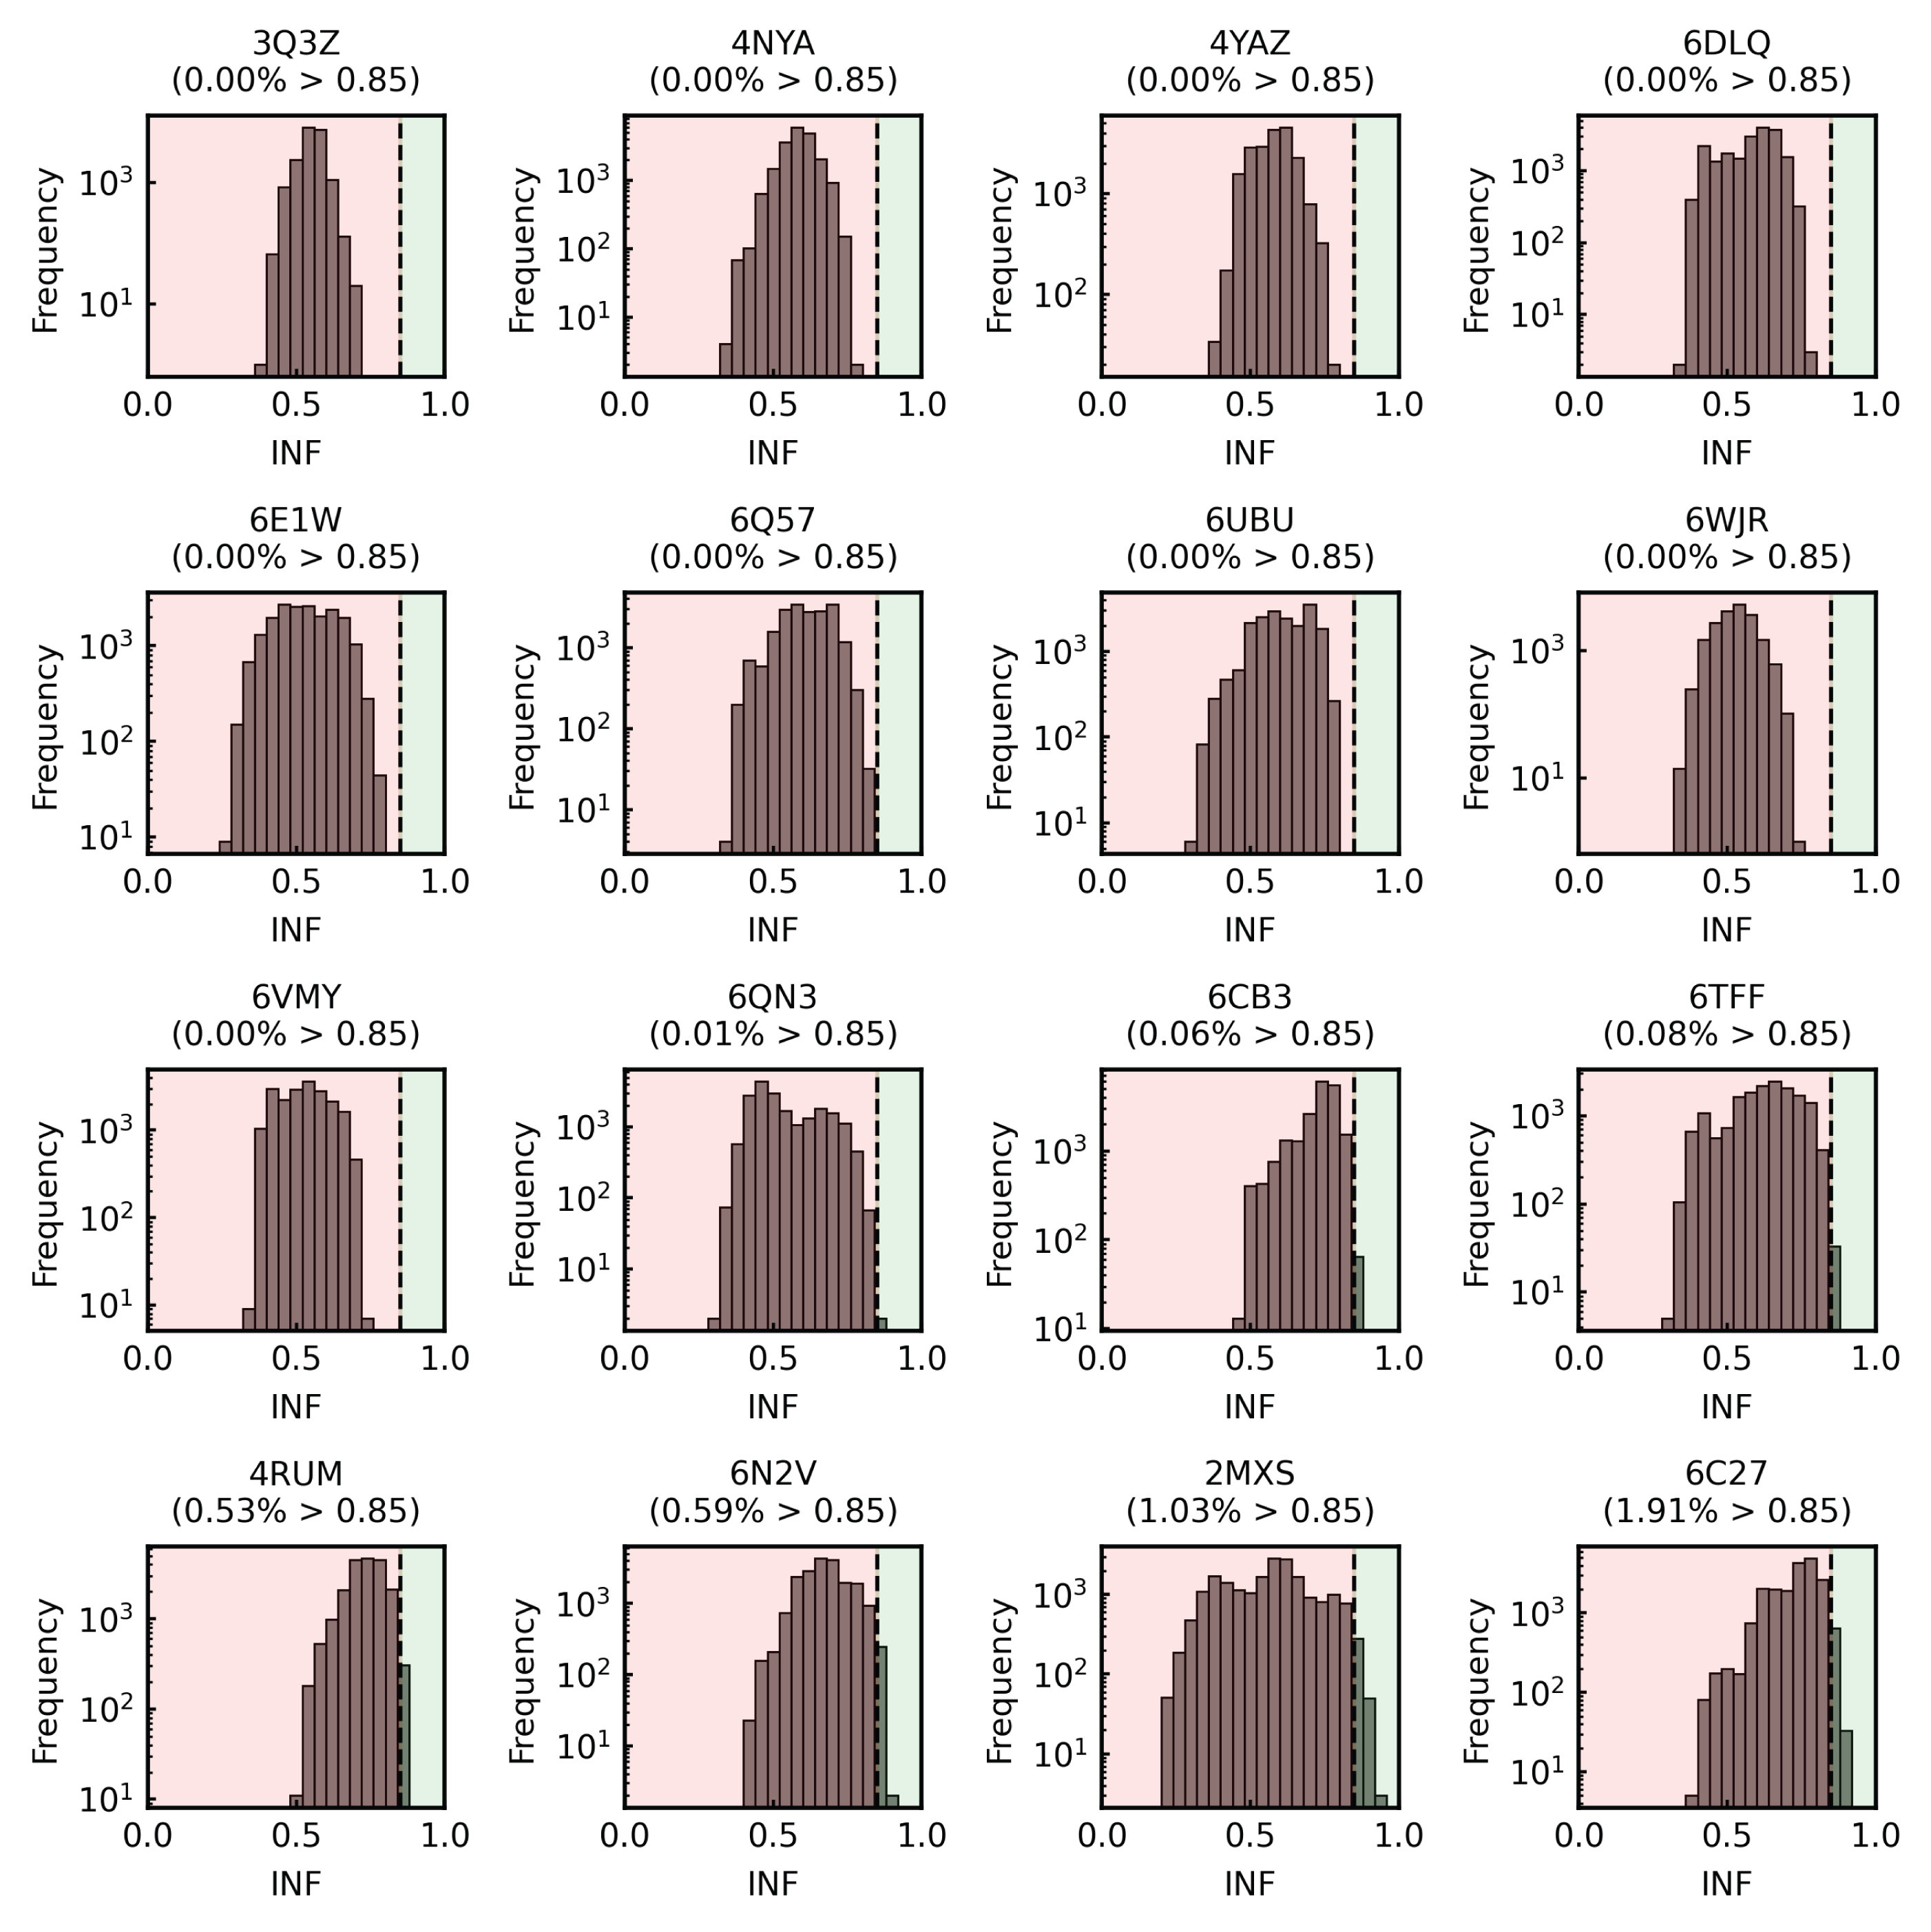
\includegraphics[
    width=0.9\textwidth
    ]{./inf_decoys.png}
    \caption{{\bf INF distribution of conformations generated by RNAnneal.} The dashed line placed at $0.85$ indicates the cutoff used to classify ``realistic'' (INF$\geq$0.85) and (INF$<$0.85) ``decoy'' conformations. The proportion of realistic conformations is provided underneath the PDB accession code.}
    \label{fig:inf_decoys}%
\end{figure}

\begin{figure}
    \centering
    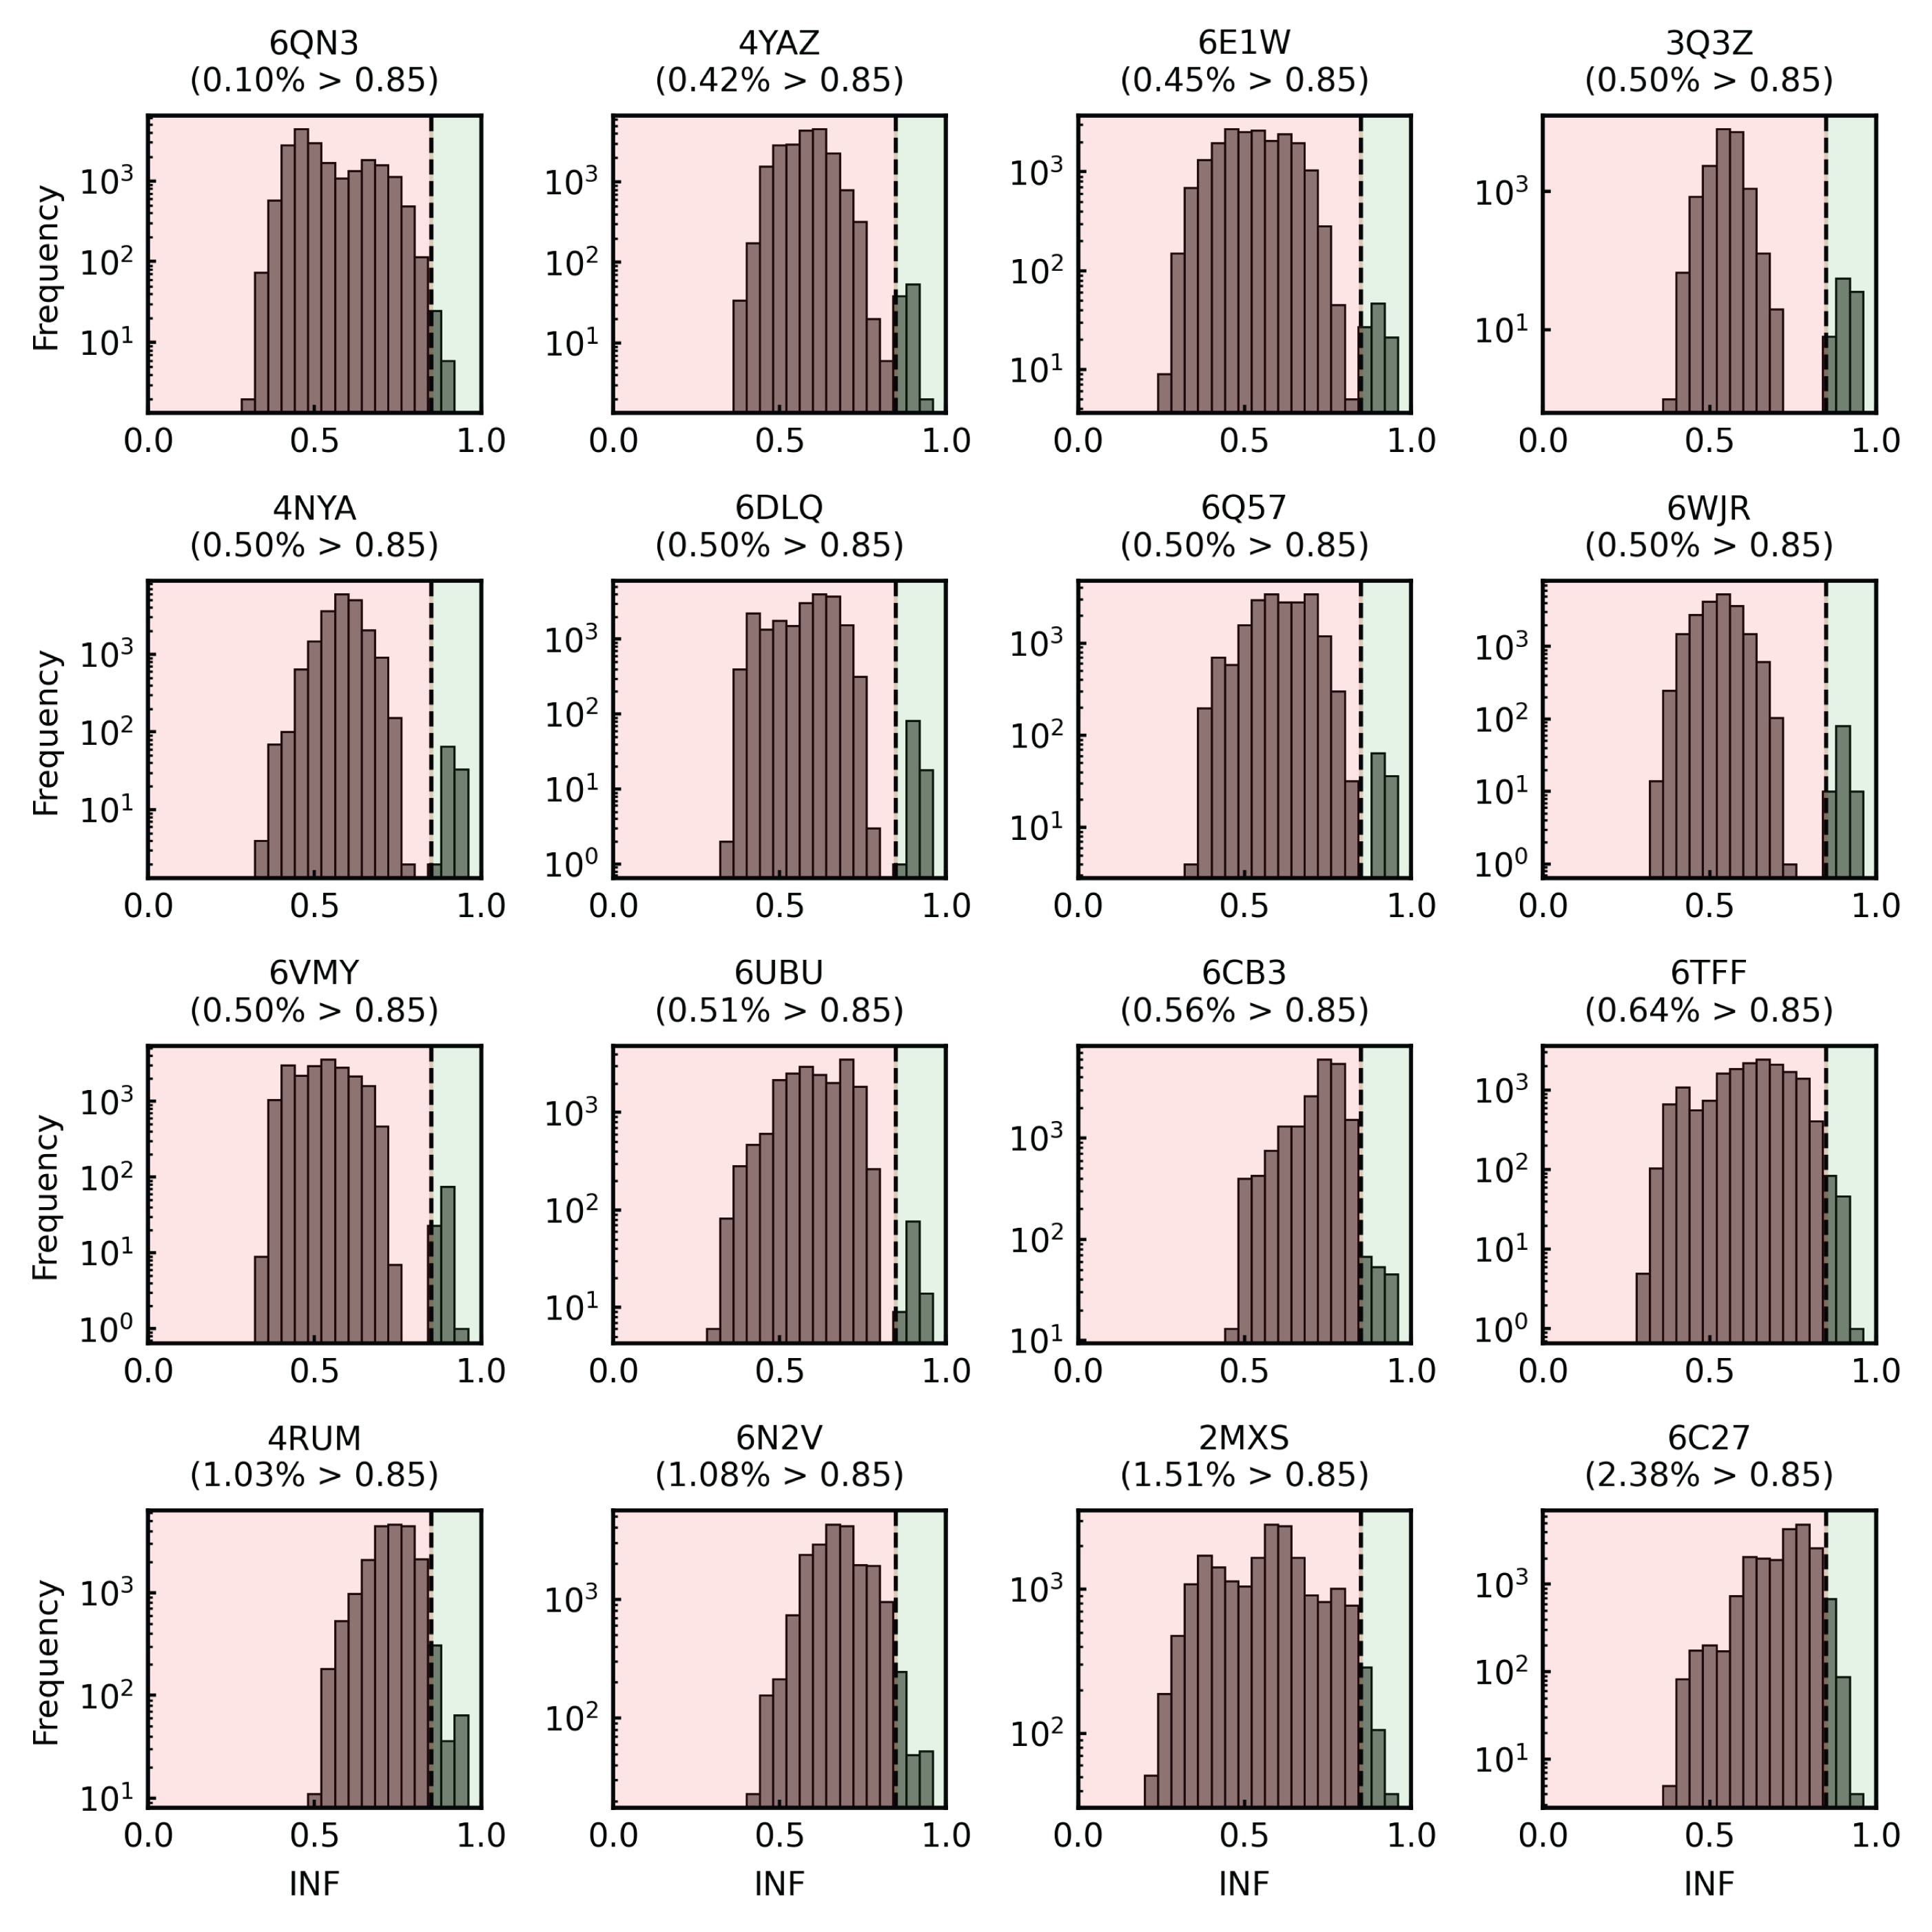
\includegraphics[
    width=0.9\textwidth
    ]{./inf_combined.png}
    \caption{{\bf INF distribution of conformations for the classification task.} The classification task merges structures sampled by RNAnneal with frames from simulations launched from the reference conformations (i.e., merges Fig. S\ref{fig:inf_reference} and S\ref{fig:inf_decoys}). The dashed line placed at $0.85$ indicates the cutoff used to classify ``realistic'' (INF$\geq$0.85) and (INF$<$0.85) ``decoy'' conformations. The proportion of realistic conformations is provided underneath the PDB accession code.}
    \label{fig:inf_combined}%
\end{figure}

\begin{figure}
    \centering
    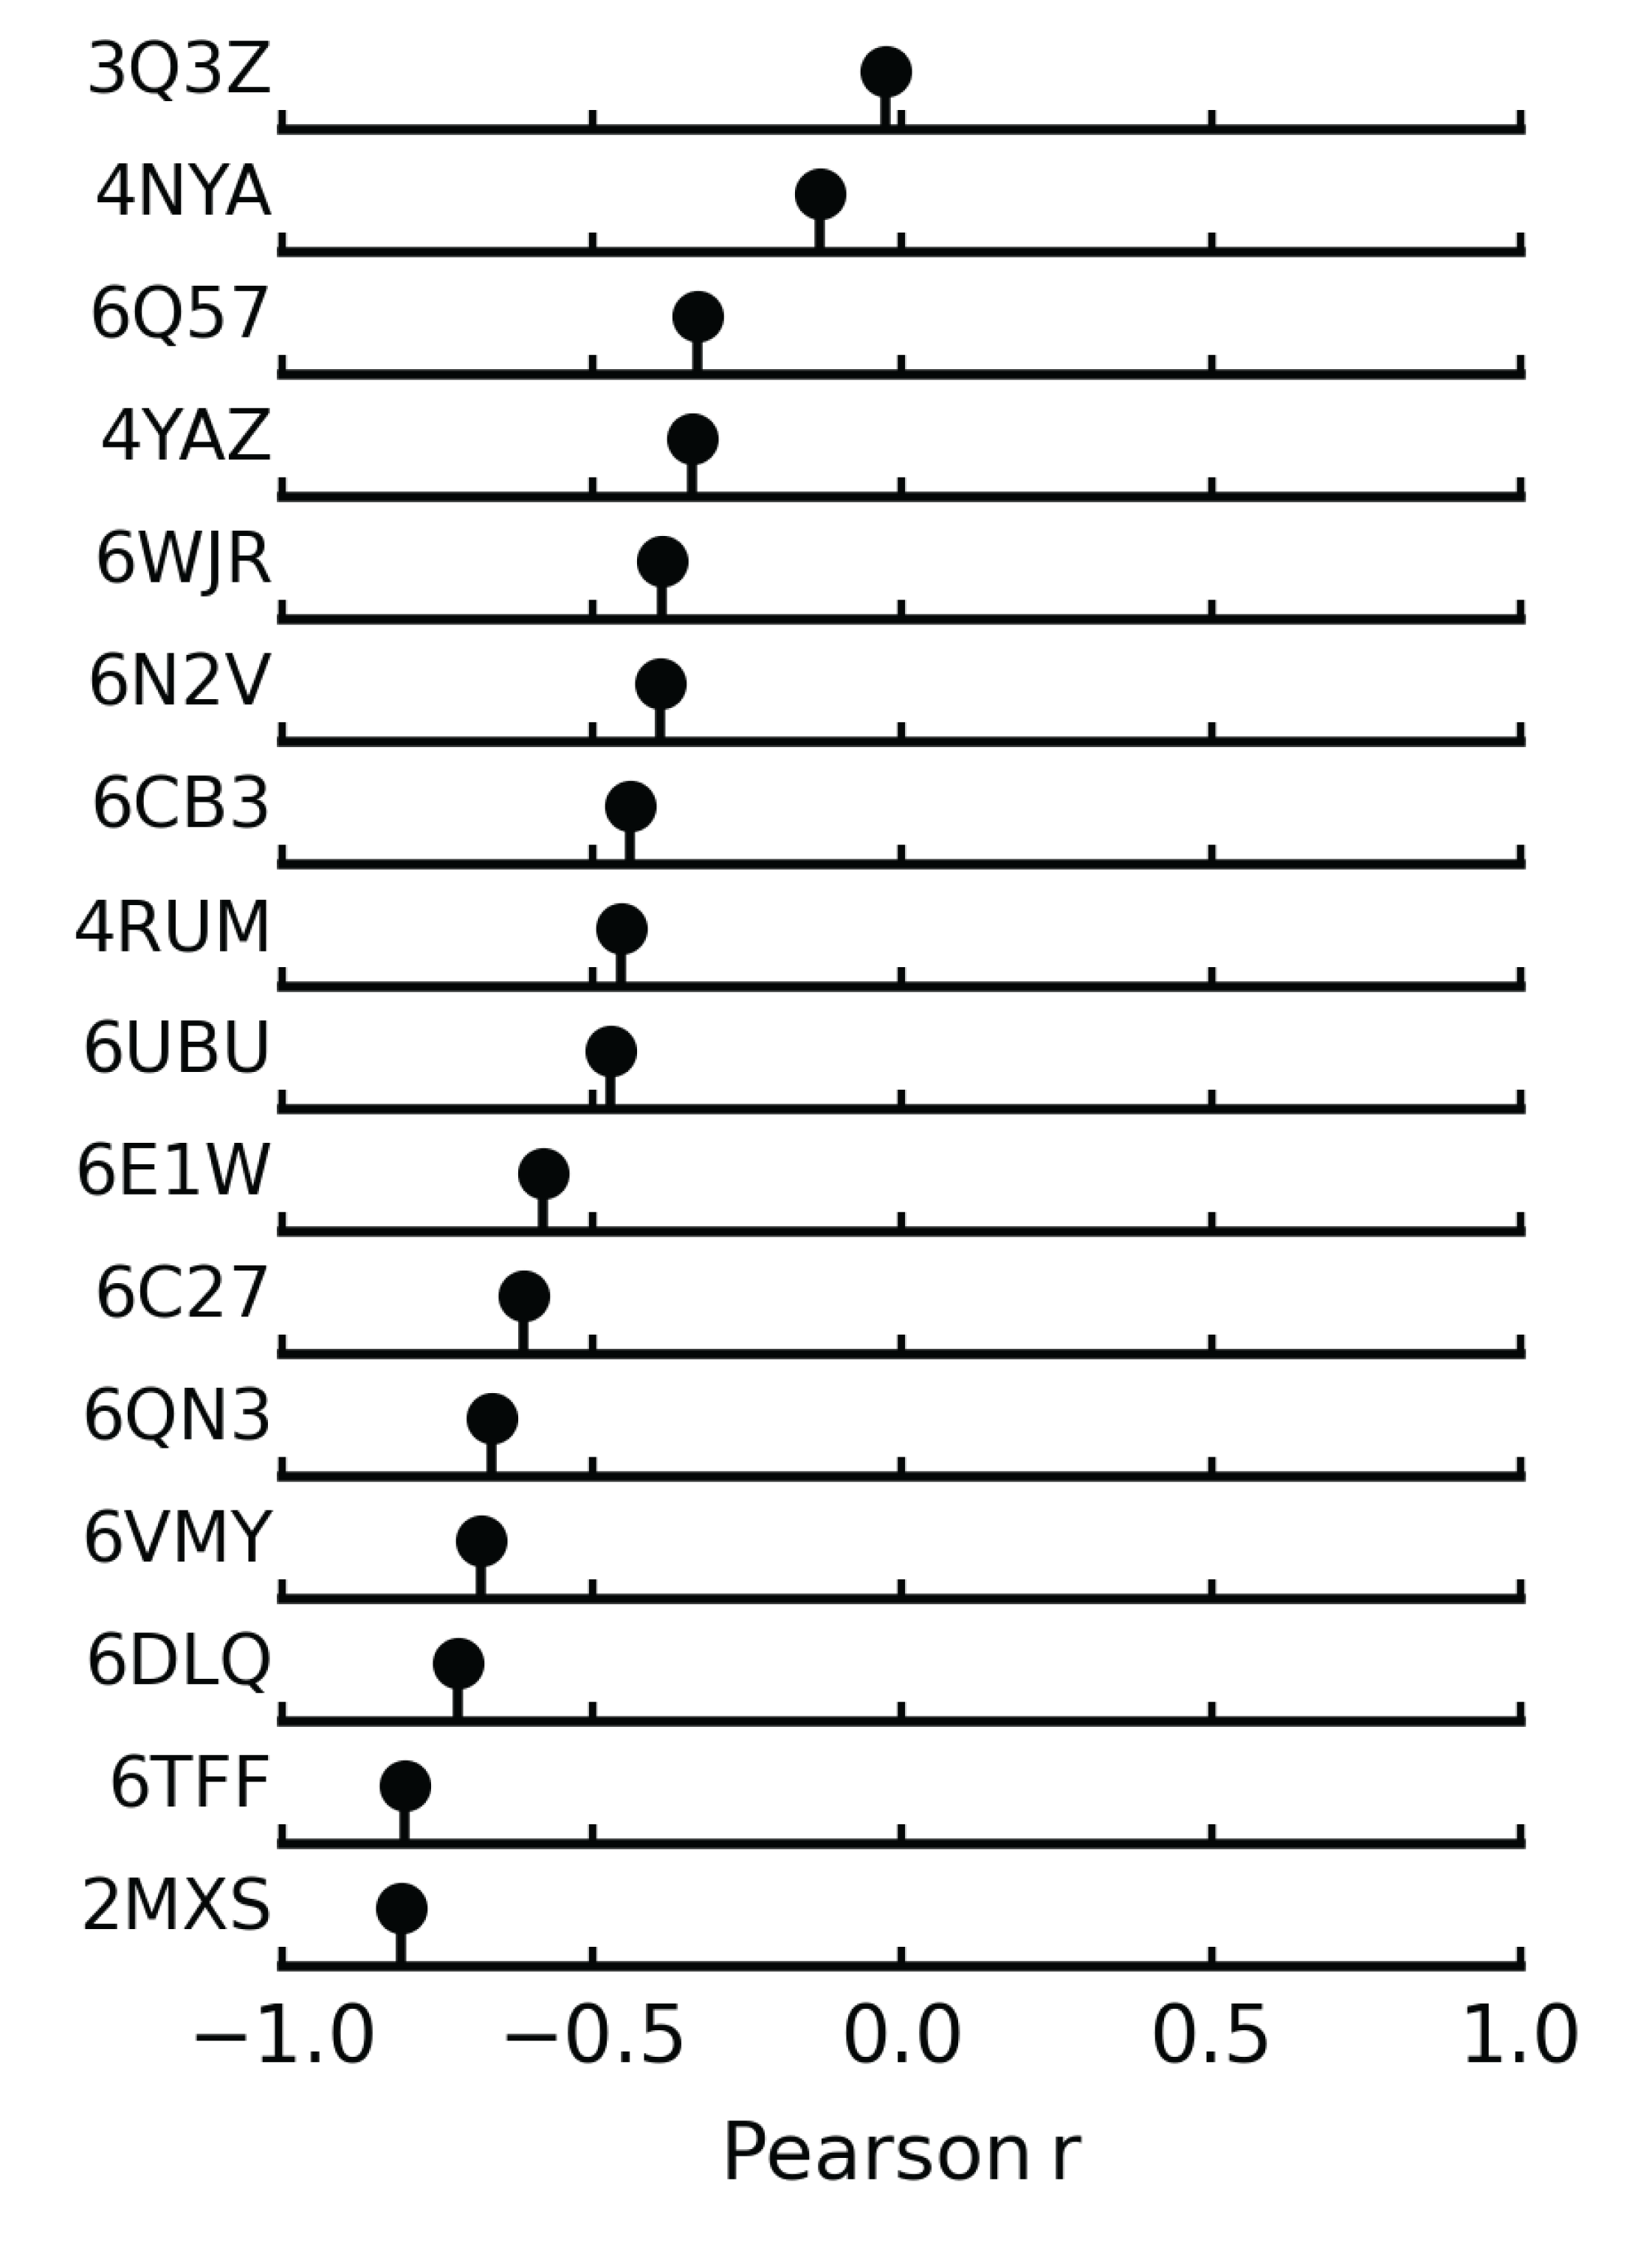
\includegraphics[
    width=0.4\textwidth
    ]{./correlation.png}
    \caption{{\bf Correlation between RMSD and INF for RNAnneal conformations.}}
    \label{fig:correlation}%
\end{figure}

\begin{figure*}
    \centering
    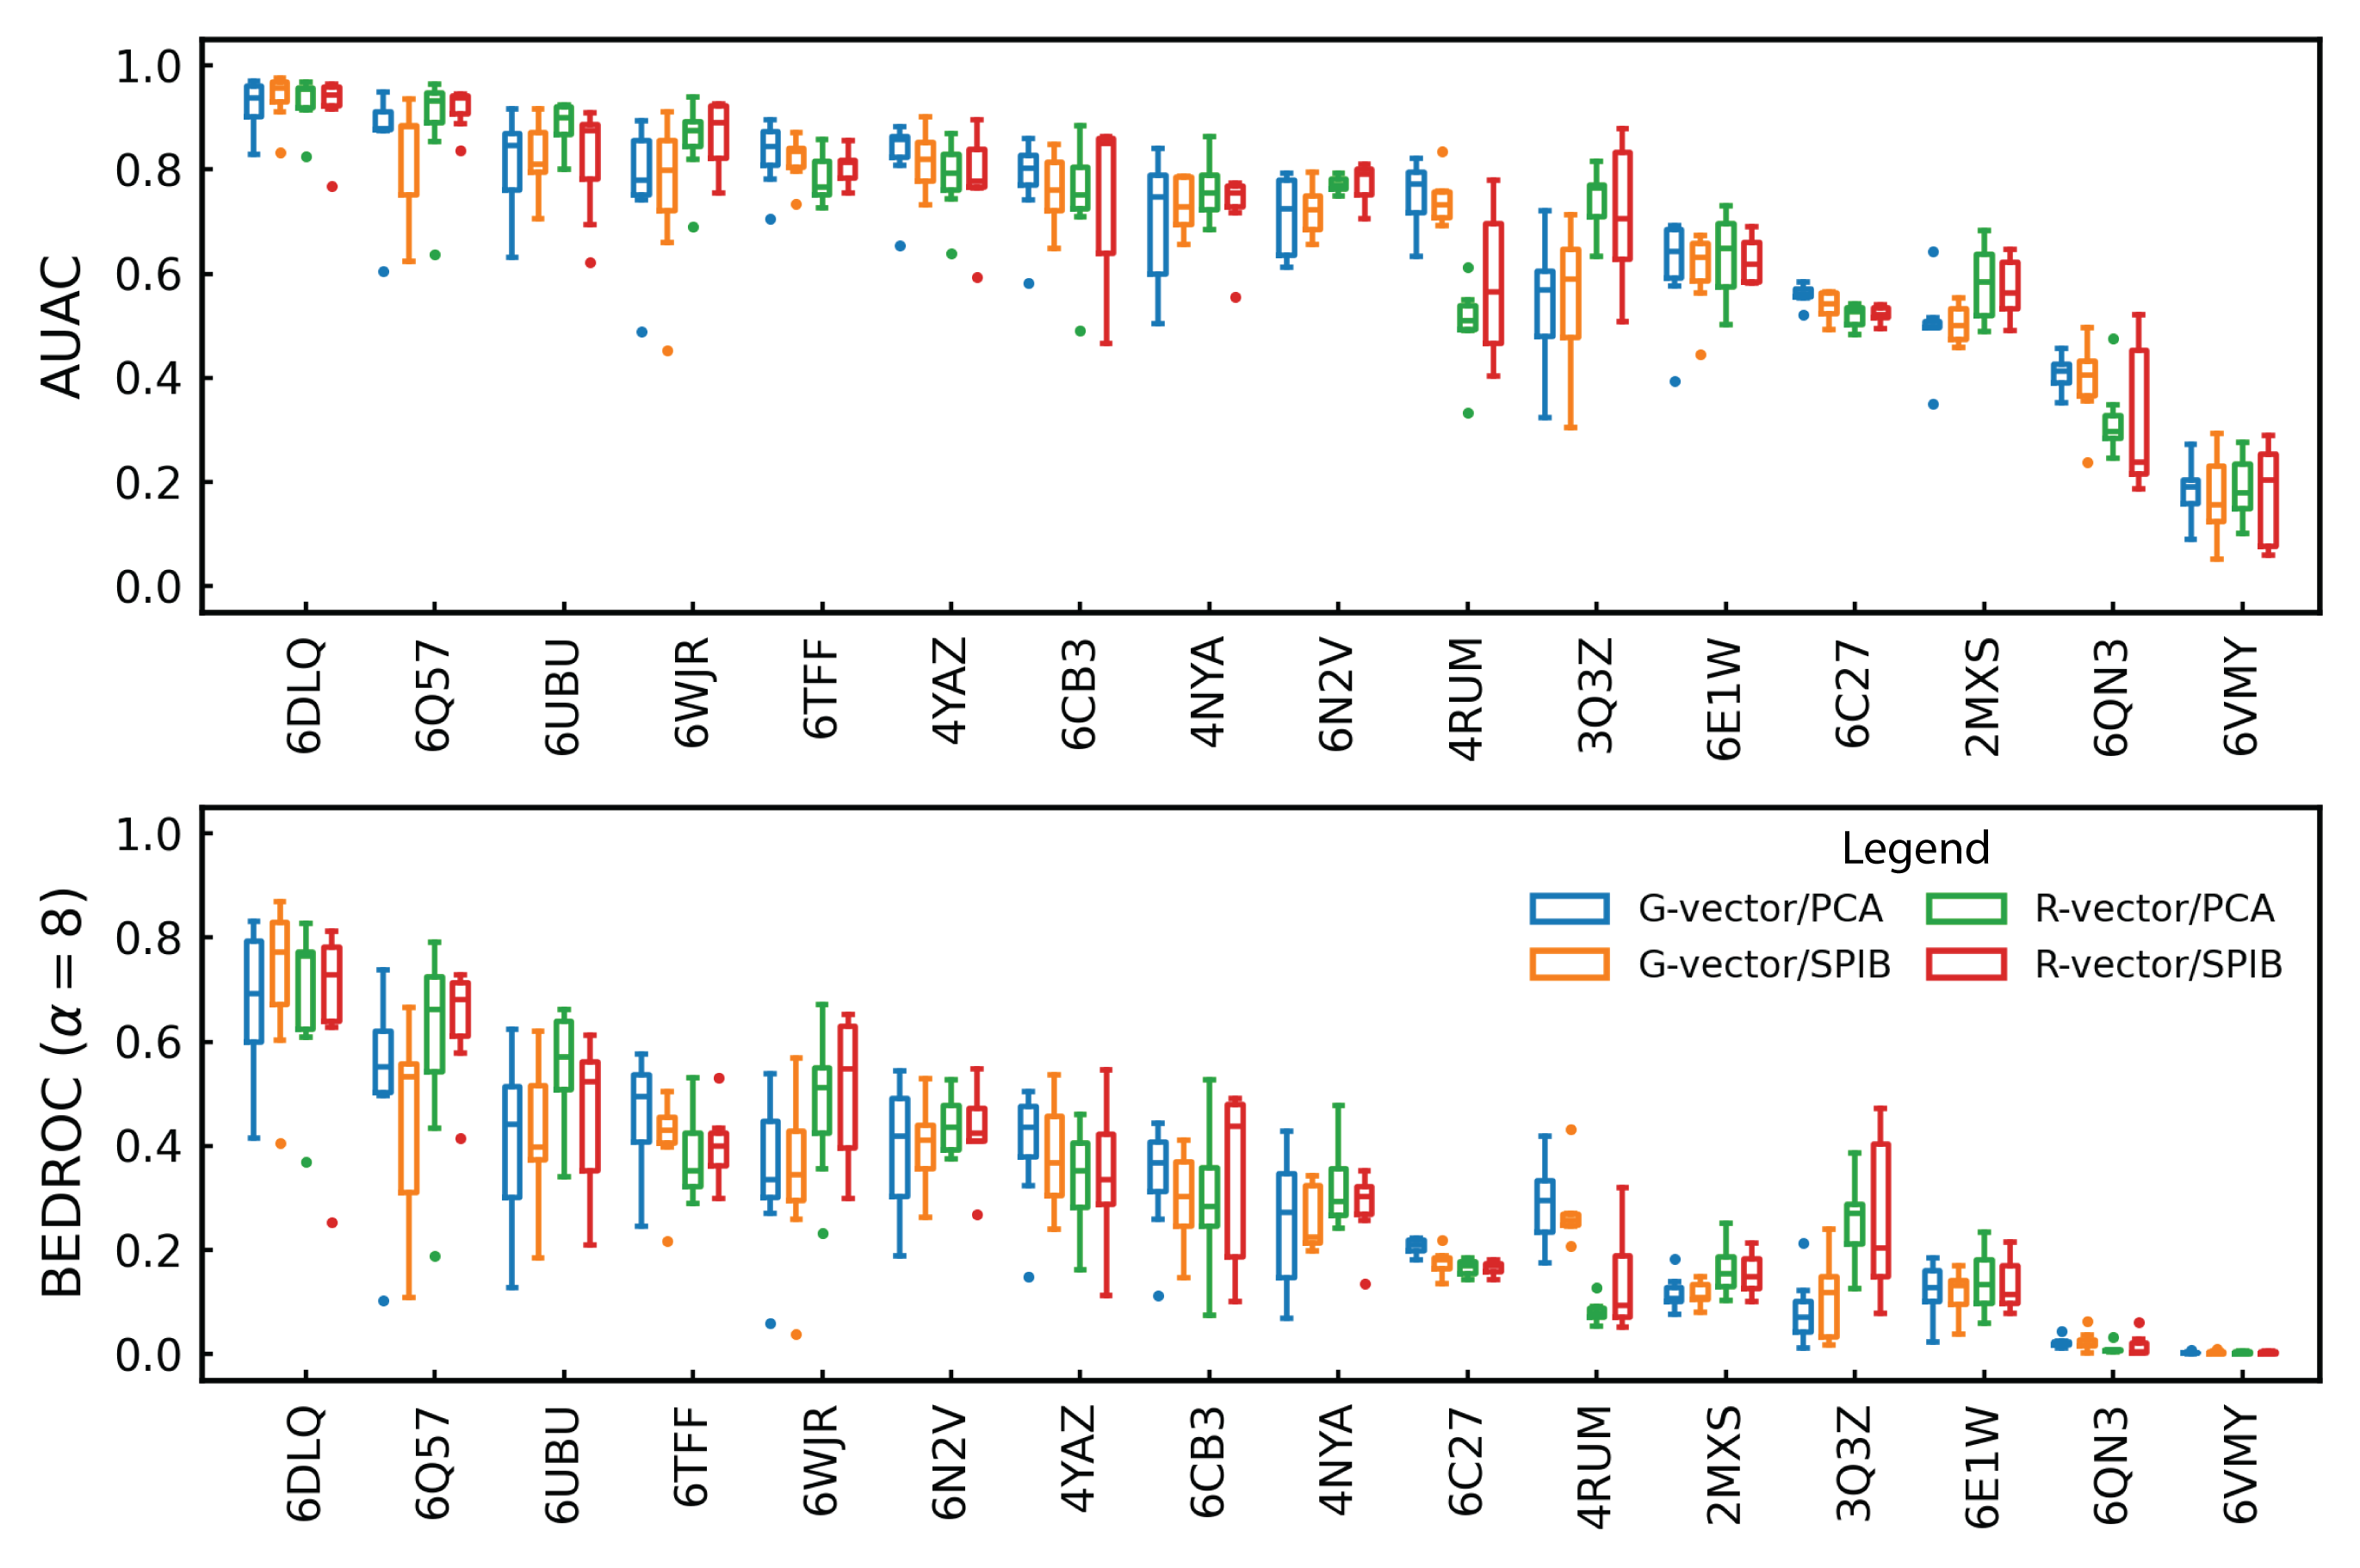
\includegraphics[
    width=0.9\textwidth
    ]{./auac-bedroc-by-feature.png}
    \caption{{\bf AUAC and BEDROC for each combination of training features.}}
    \label{fig:classification-by-feature}%
\end{figure*}

\begin{figure*}
    \centering
    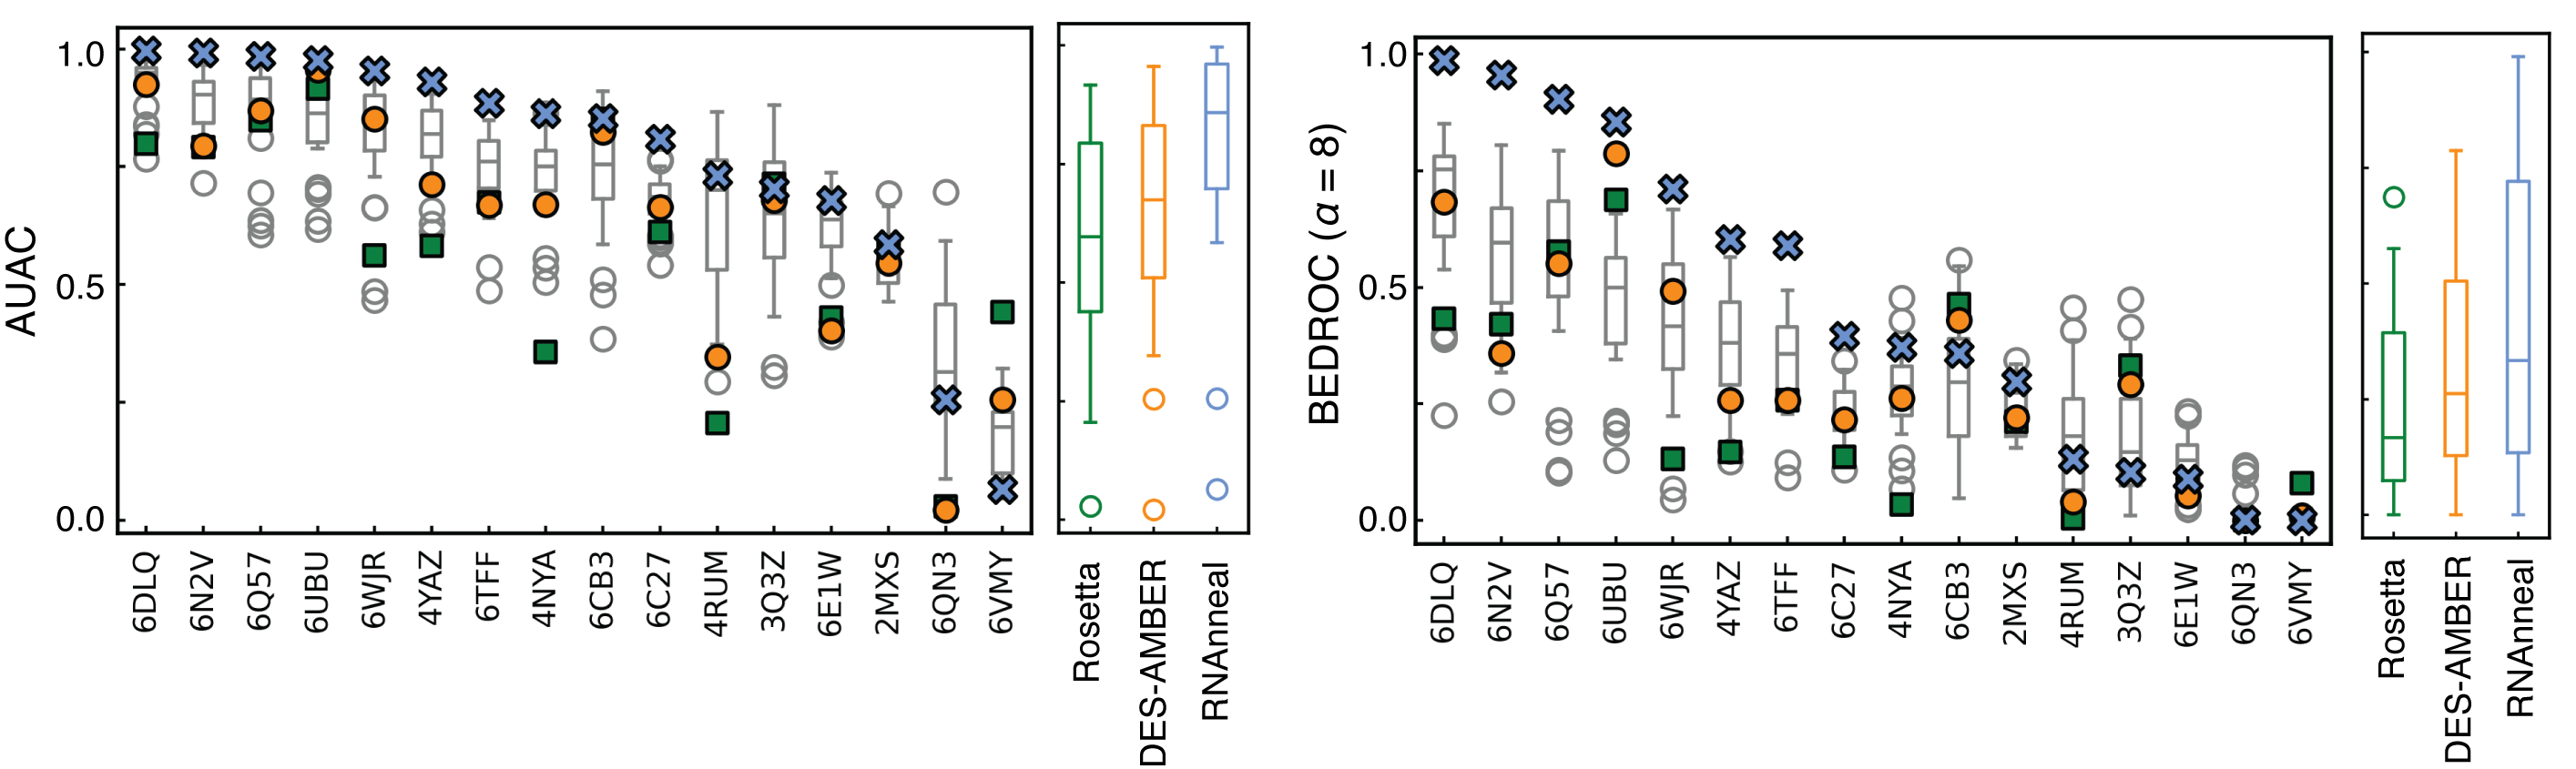
\includegraphics[
    width=\textwidth
    ]{./rmsd-enrichment.png}
    \caption{{\bf AUAC and BEDROC for RMSD classification criteria.} Classification power of the Rosetta (blue), DES-AMBER (orange), and RNAnneal (blue) scores when ERCs are defined as conformations $<5${\AA} in RMSD from the reference conformation. The gray boxplots show the distribution of AUAC and BEDROC values for each model in the TM ensemble.}
    \label{fig:rmsd-enrichment}%
\end{figure*}

\begin{figure}
    \centering
    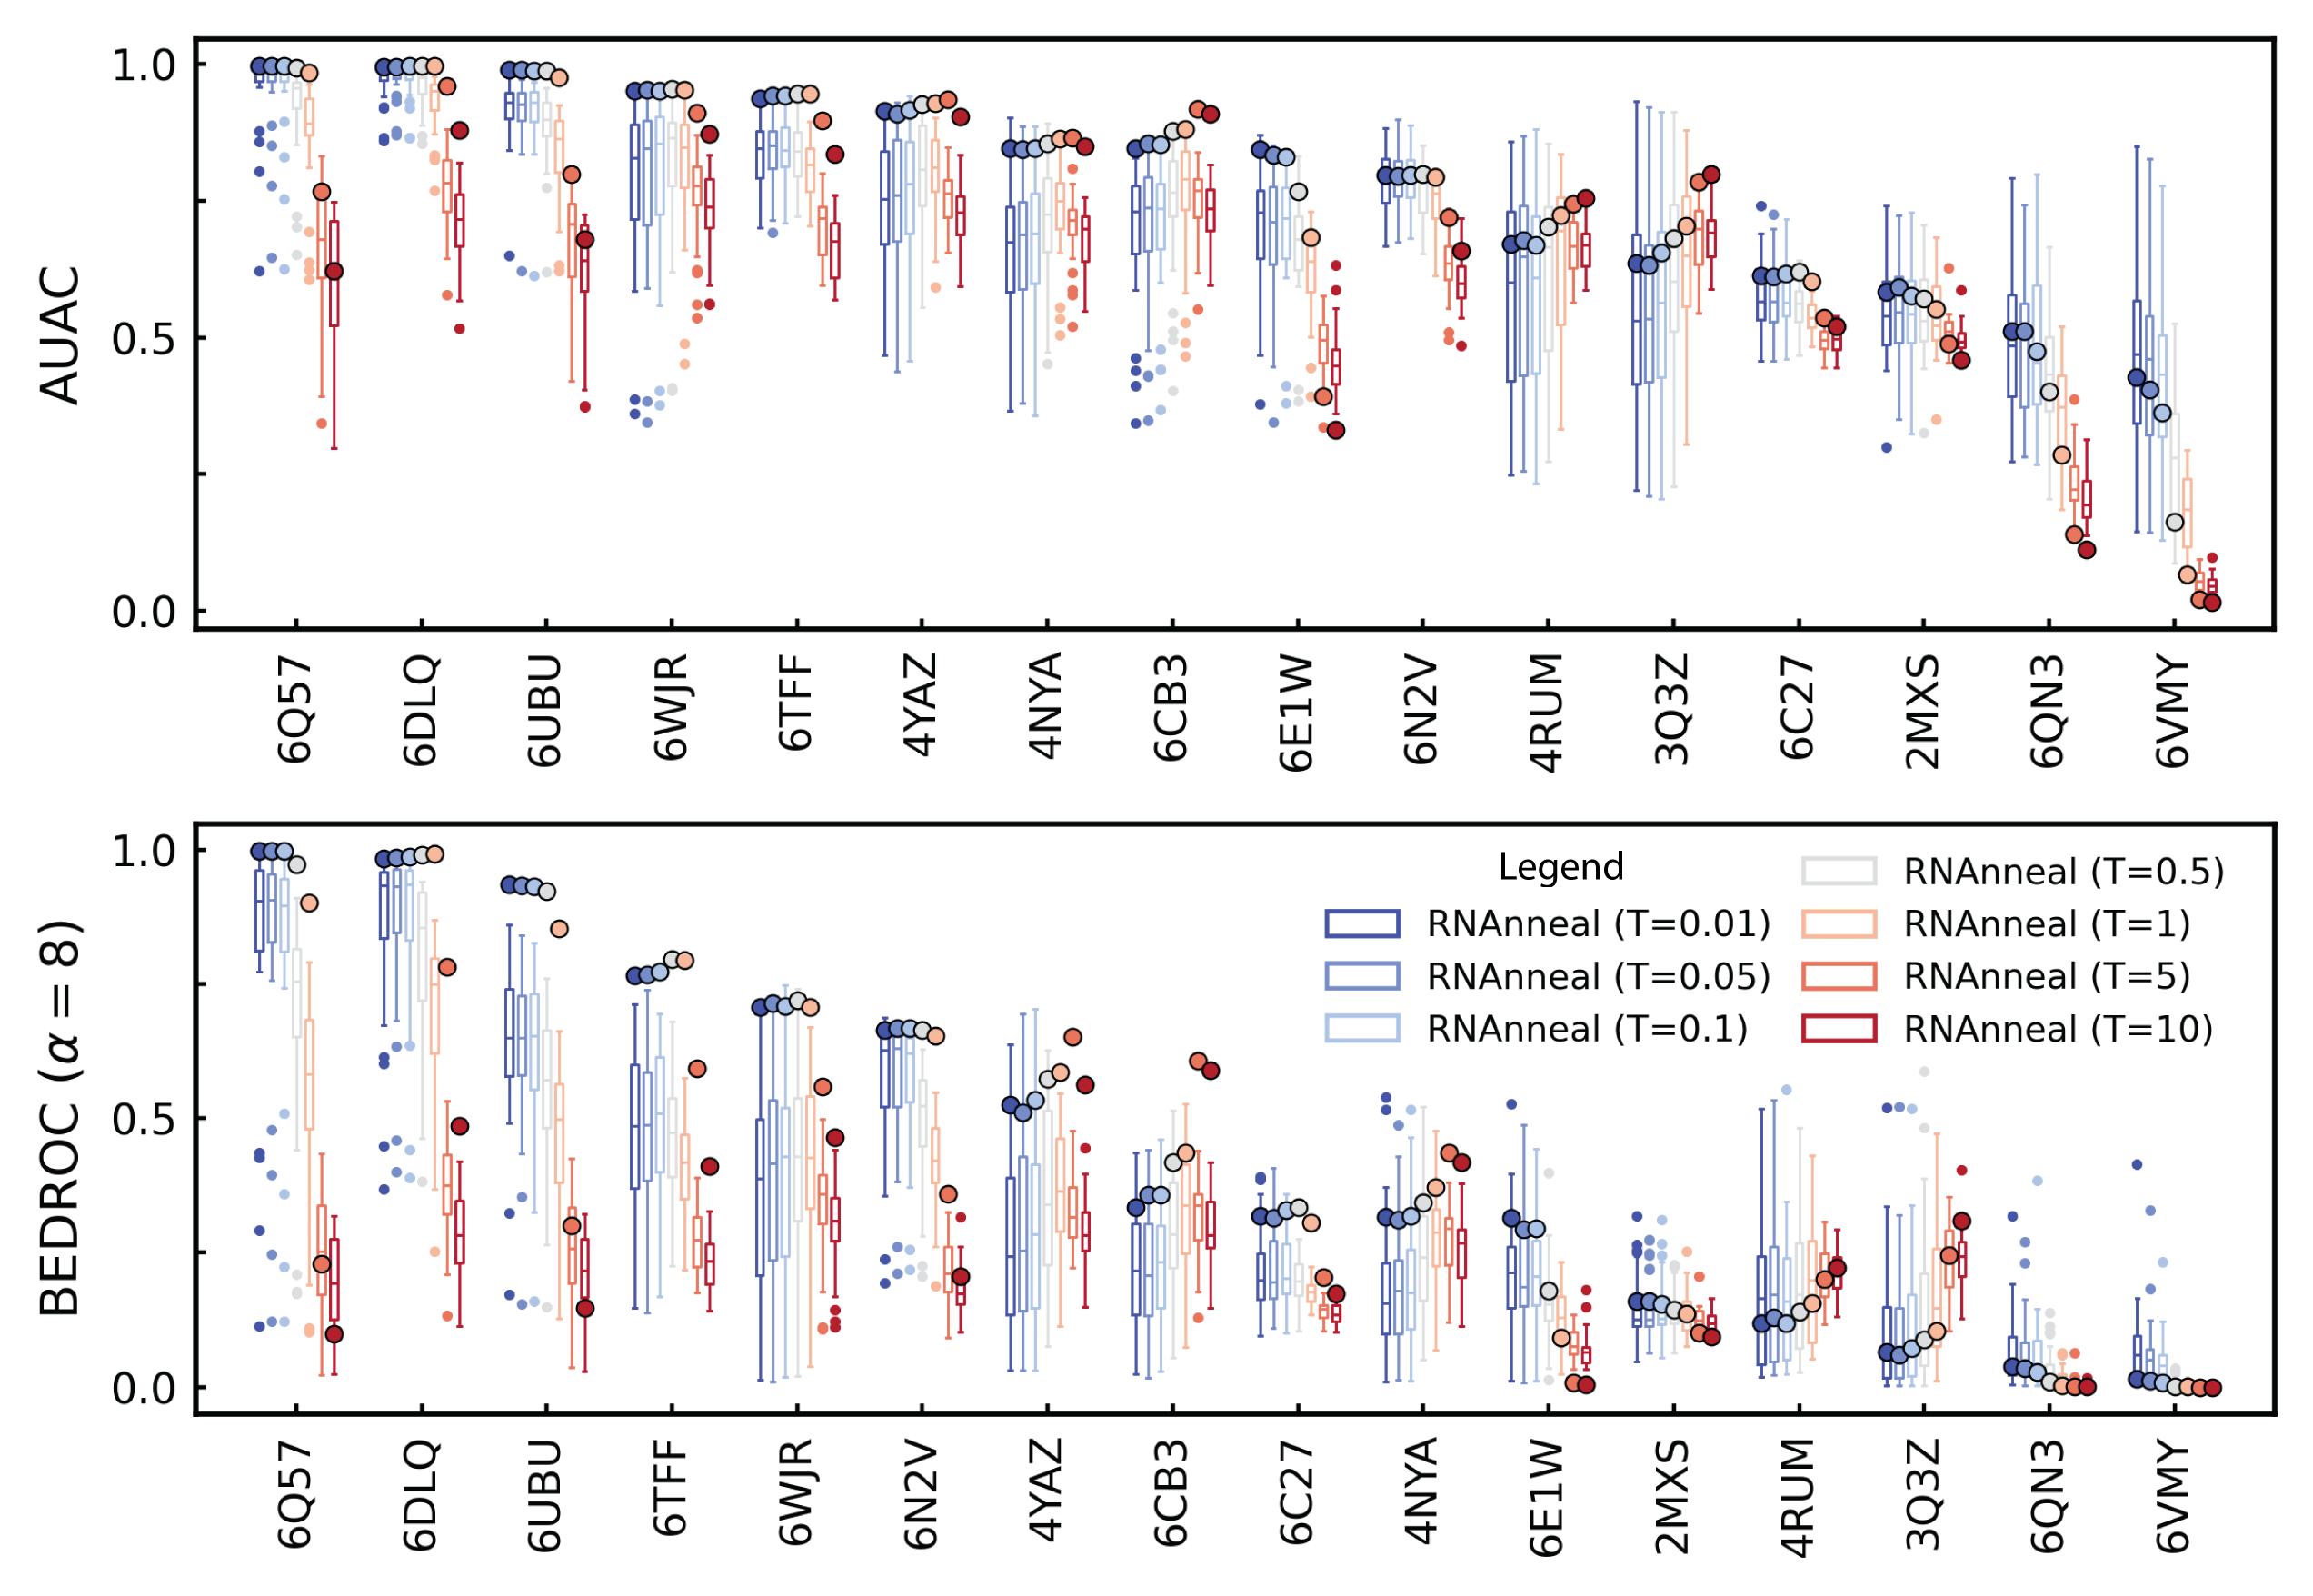
\includegraphics[
    width=0.9\textwidth
    ]{./enrichment-temperature-dependence.png}
    \caption{{\bf Variation in AUAC and BEDROC with scoring temperature.}}
    \label{fig:model-temp-dependence}%
\end{figure}

% \begin{figure*}
%     \centering
%     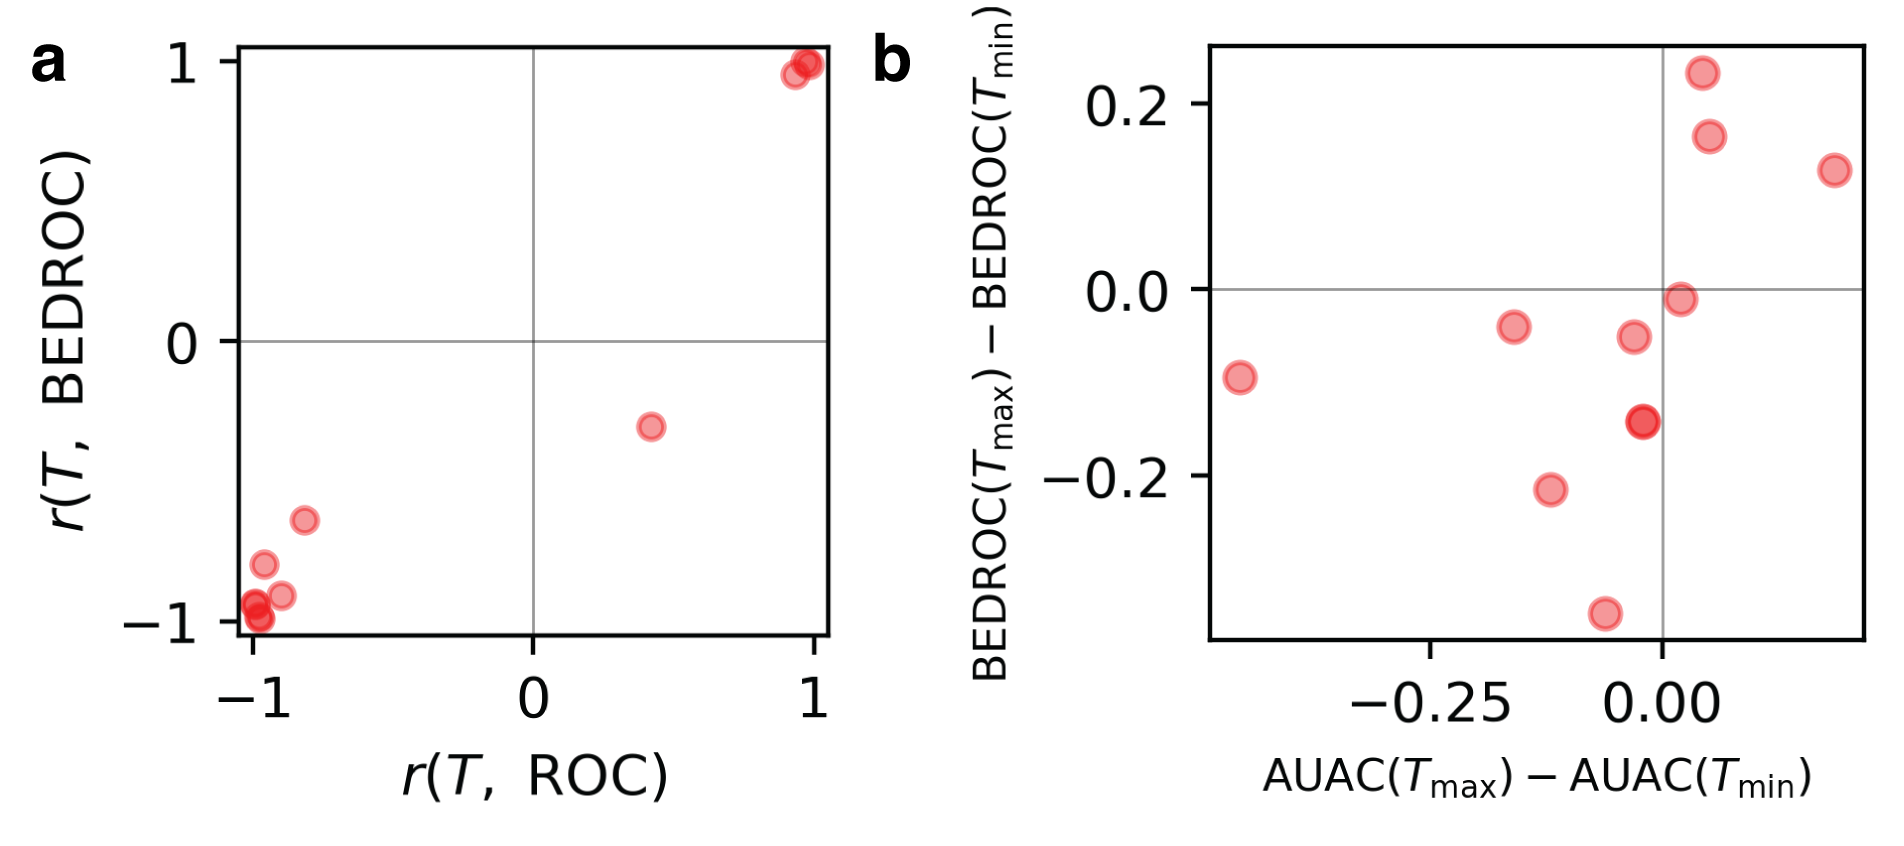
\includegraphics[
%     width=0.75\textwidth
%     ]{./auac-bedroc-temperature-analysis.png}
%     \caption{{\bf The effect of model temperature on AUAC and BEDROC} (a) The correlation between AUAC and BEDROC values and model temperature $T \in \{0.1, 0.5, 1.0, 1.5, 2.0, 2.5\}$ is reported. For all but three RNAs increasing temperature linearly decreases AUAC and BEDROC. (b) The difference in AUAC and BEDROC at the minimum and maximum model temperature is reported. The AUAC and BEDROC value generally decreases as the temperature is raised.}
%     \label{fig:model-temperature}%
% \end{figure*}

\begin{figure*}
    \centering
    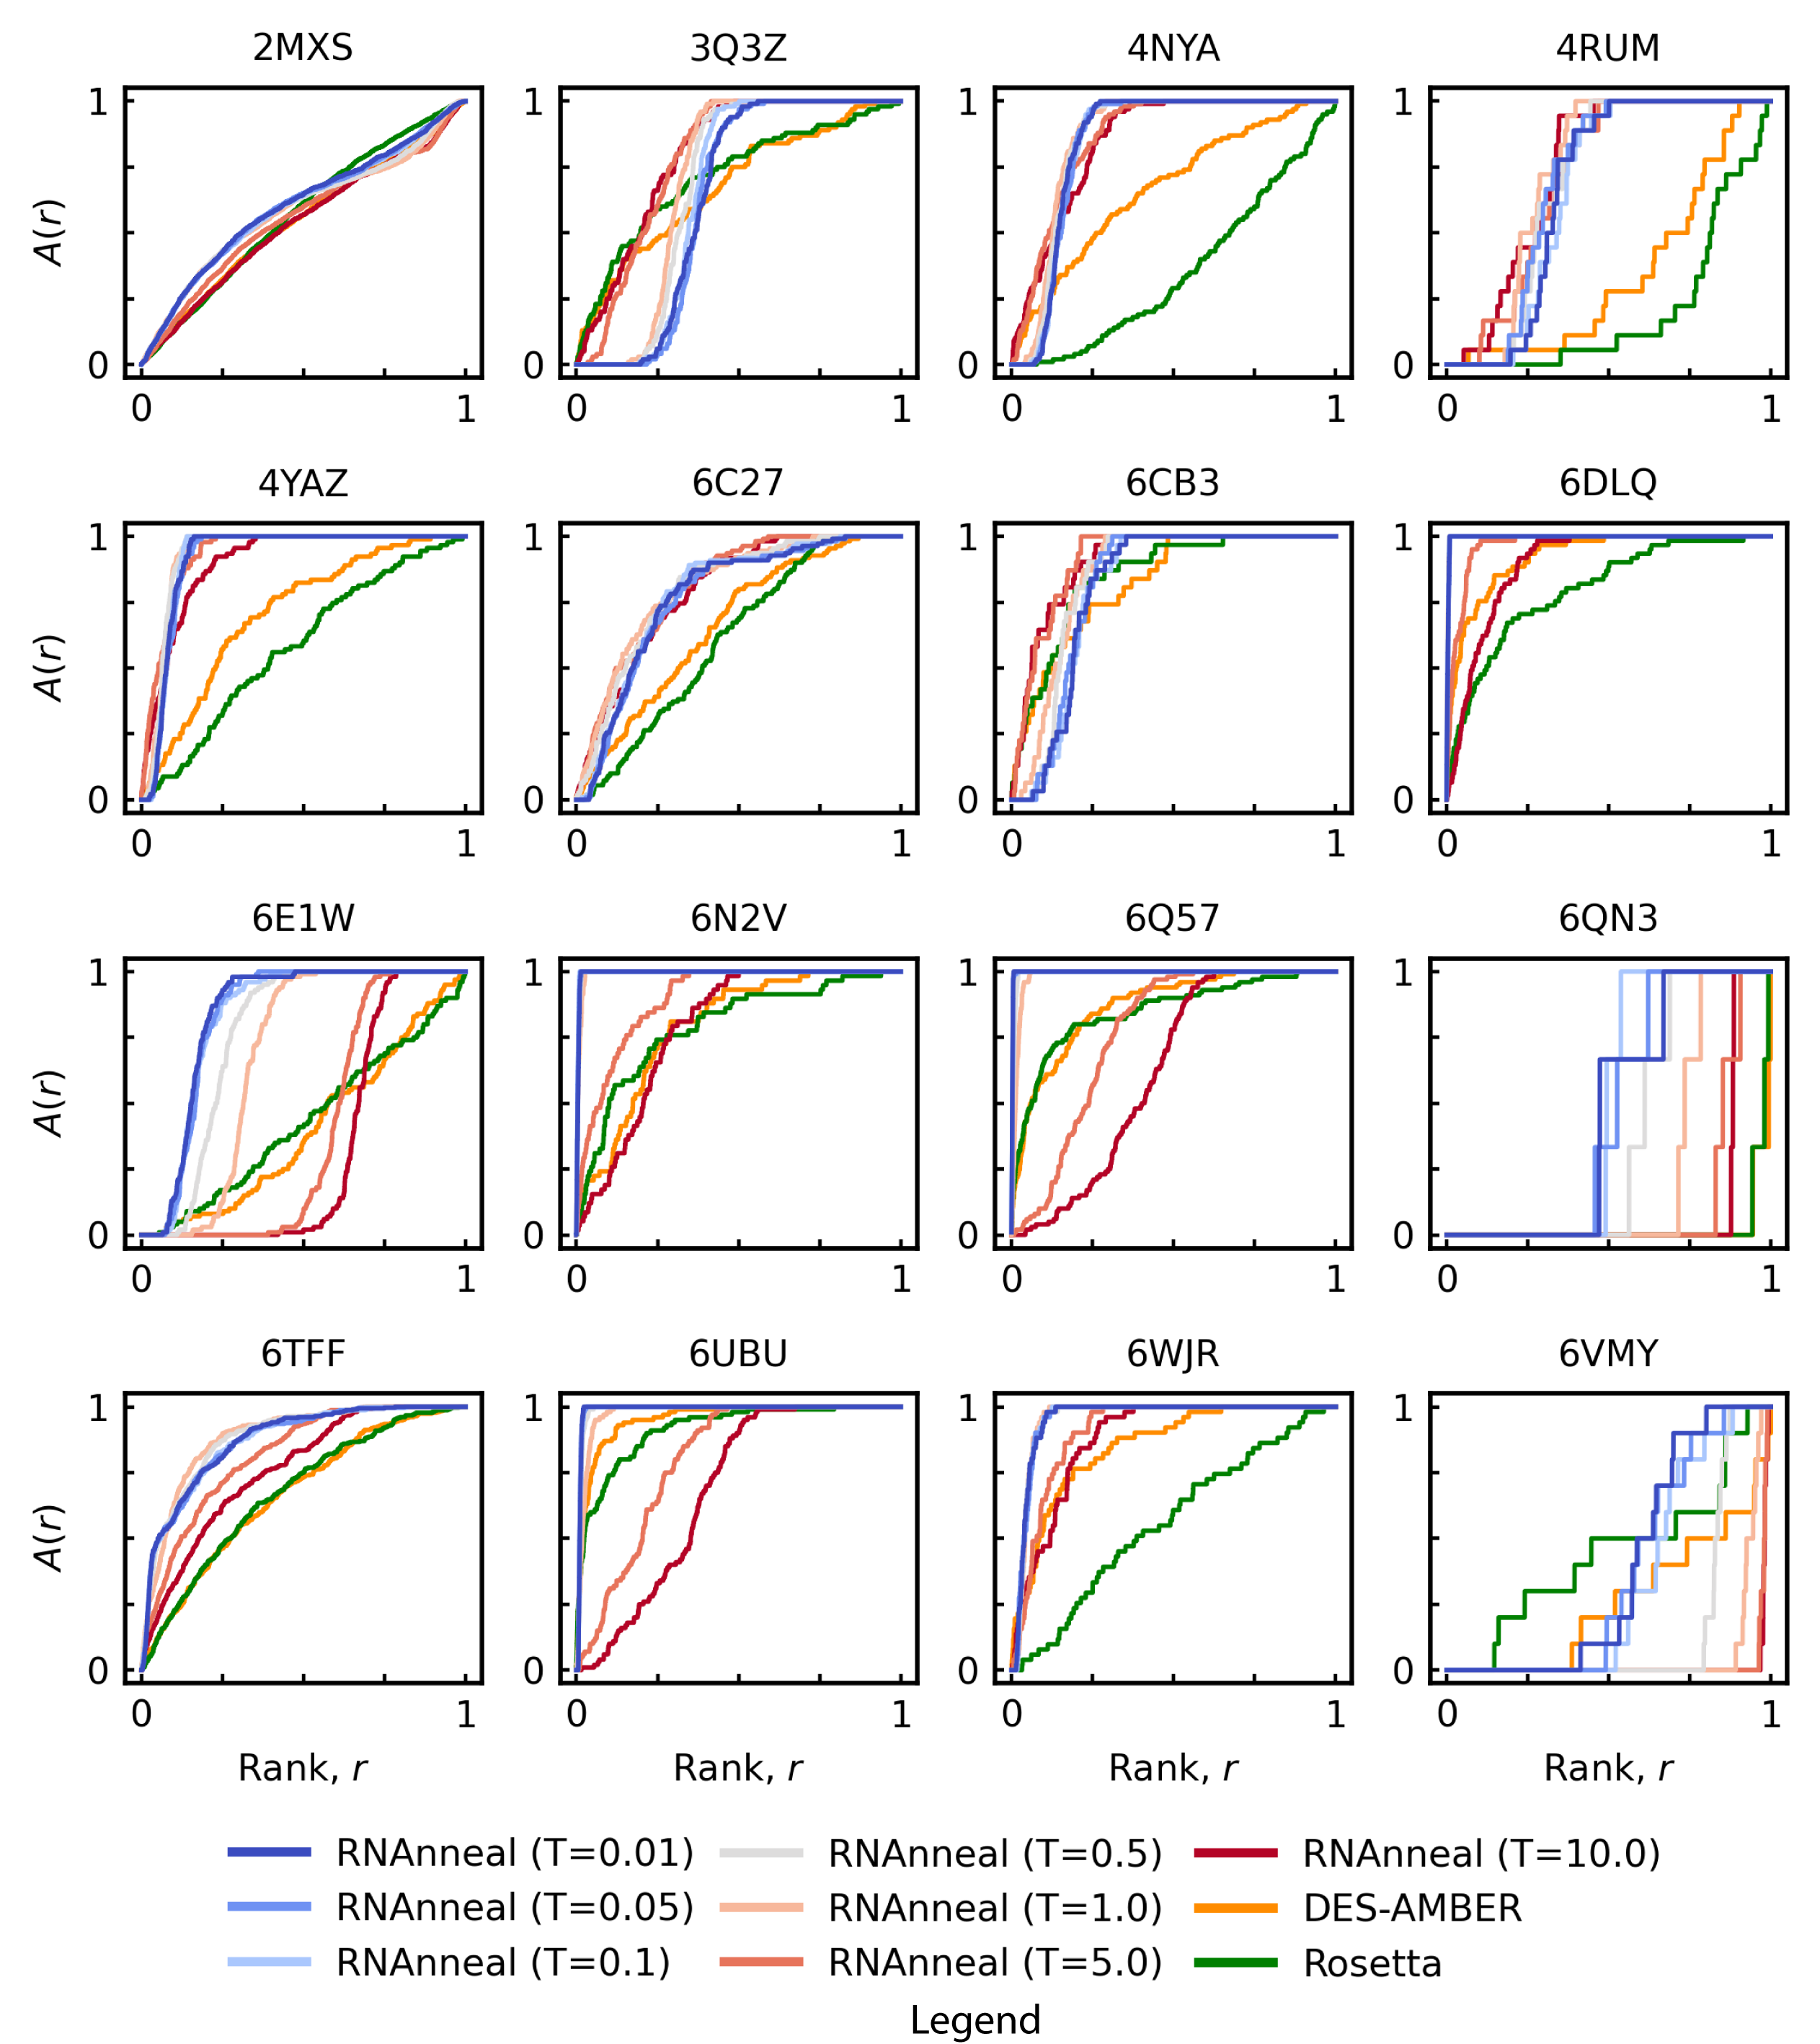
\includegraphics[
    width=\textwidth
    ]{./accum_curves_inf.png}
    \caption{{\bf Accumulation Curves.} Accumulation curves, $A(r)$ are reported for each riboswitch, identified by the PDB entry of the reference conformation.}
    \label{fig:acc-curves}%
\end{figure*}

\begin{figure*}
    \centering
    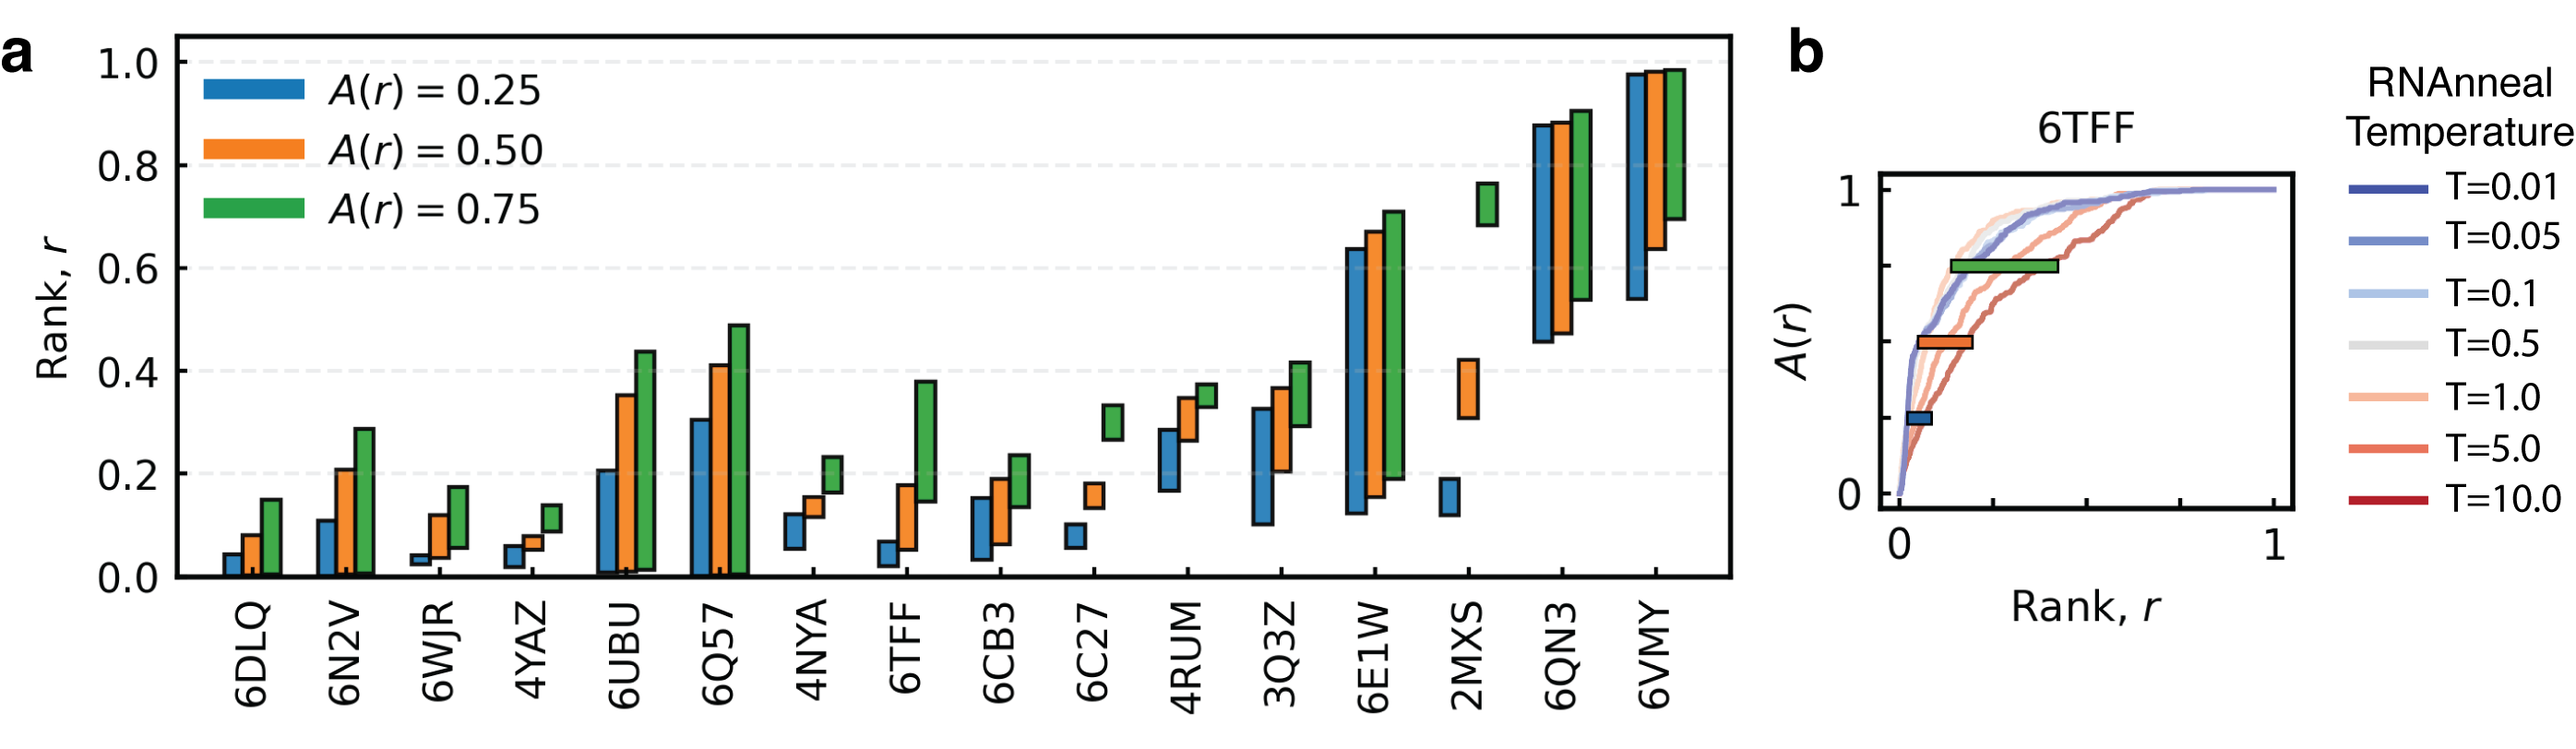
\includegraphics[
    width=\textwidth
    ]{./accumulation-curve-summary.png}
    \caption{{\bf Summary of Accumulation Curves} \textbf{a.} The set of accumulation curves for each riboswitch PDB is shown with the range of rank, $r$, for which $A(r)=0.25$, $A(r)=0.50$, and $A(r)=0.75$. \textbf{b.} The range indicated by the bars shows the variation of $r$ with temperature at fixed values of $A(r)=0.25$, $A(r)=0.50$, and $A(r)=0.75$. The accumulation curve for the PreQ1 riboswitch (6E1W) is shown as an example (see Fig. S\ref{fig:acc-curves} for all riboswitches).   }
    \label{fig:acc-curve-summary}%
\end{figure*}

\begin{figure*}
    \centering
    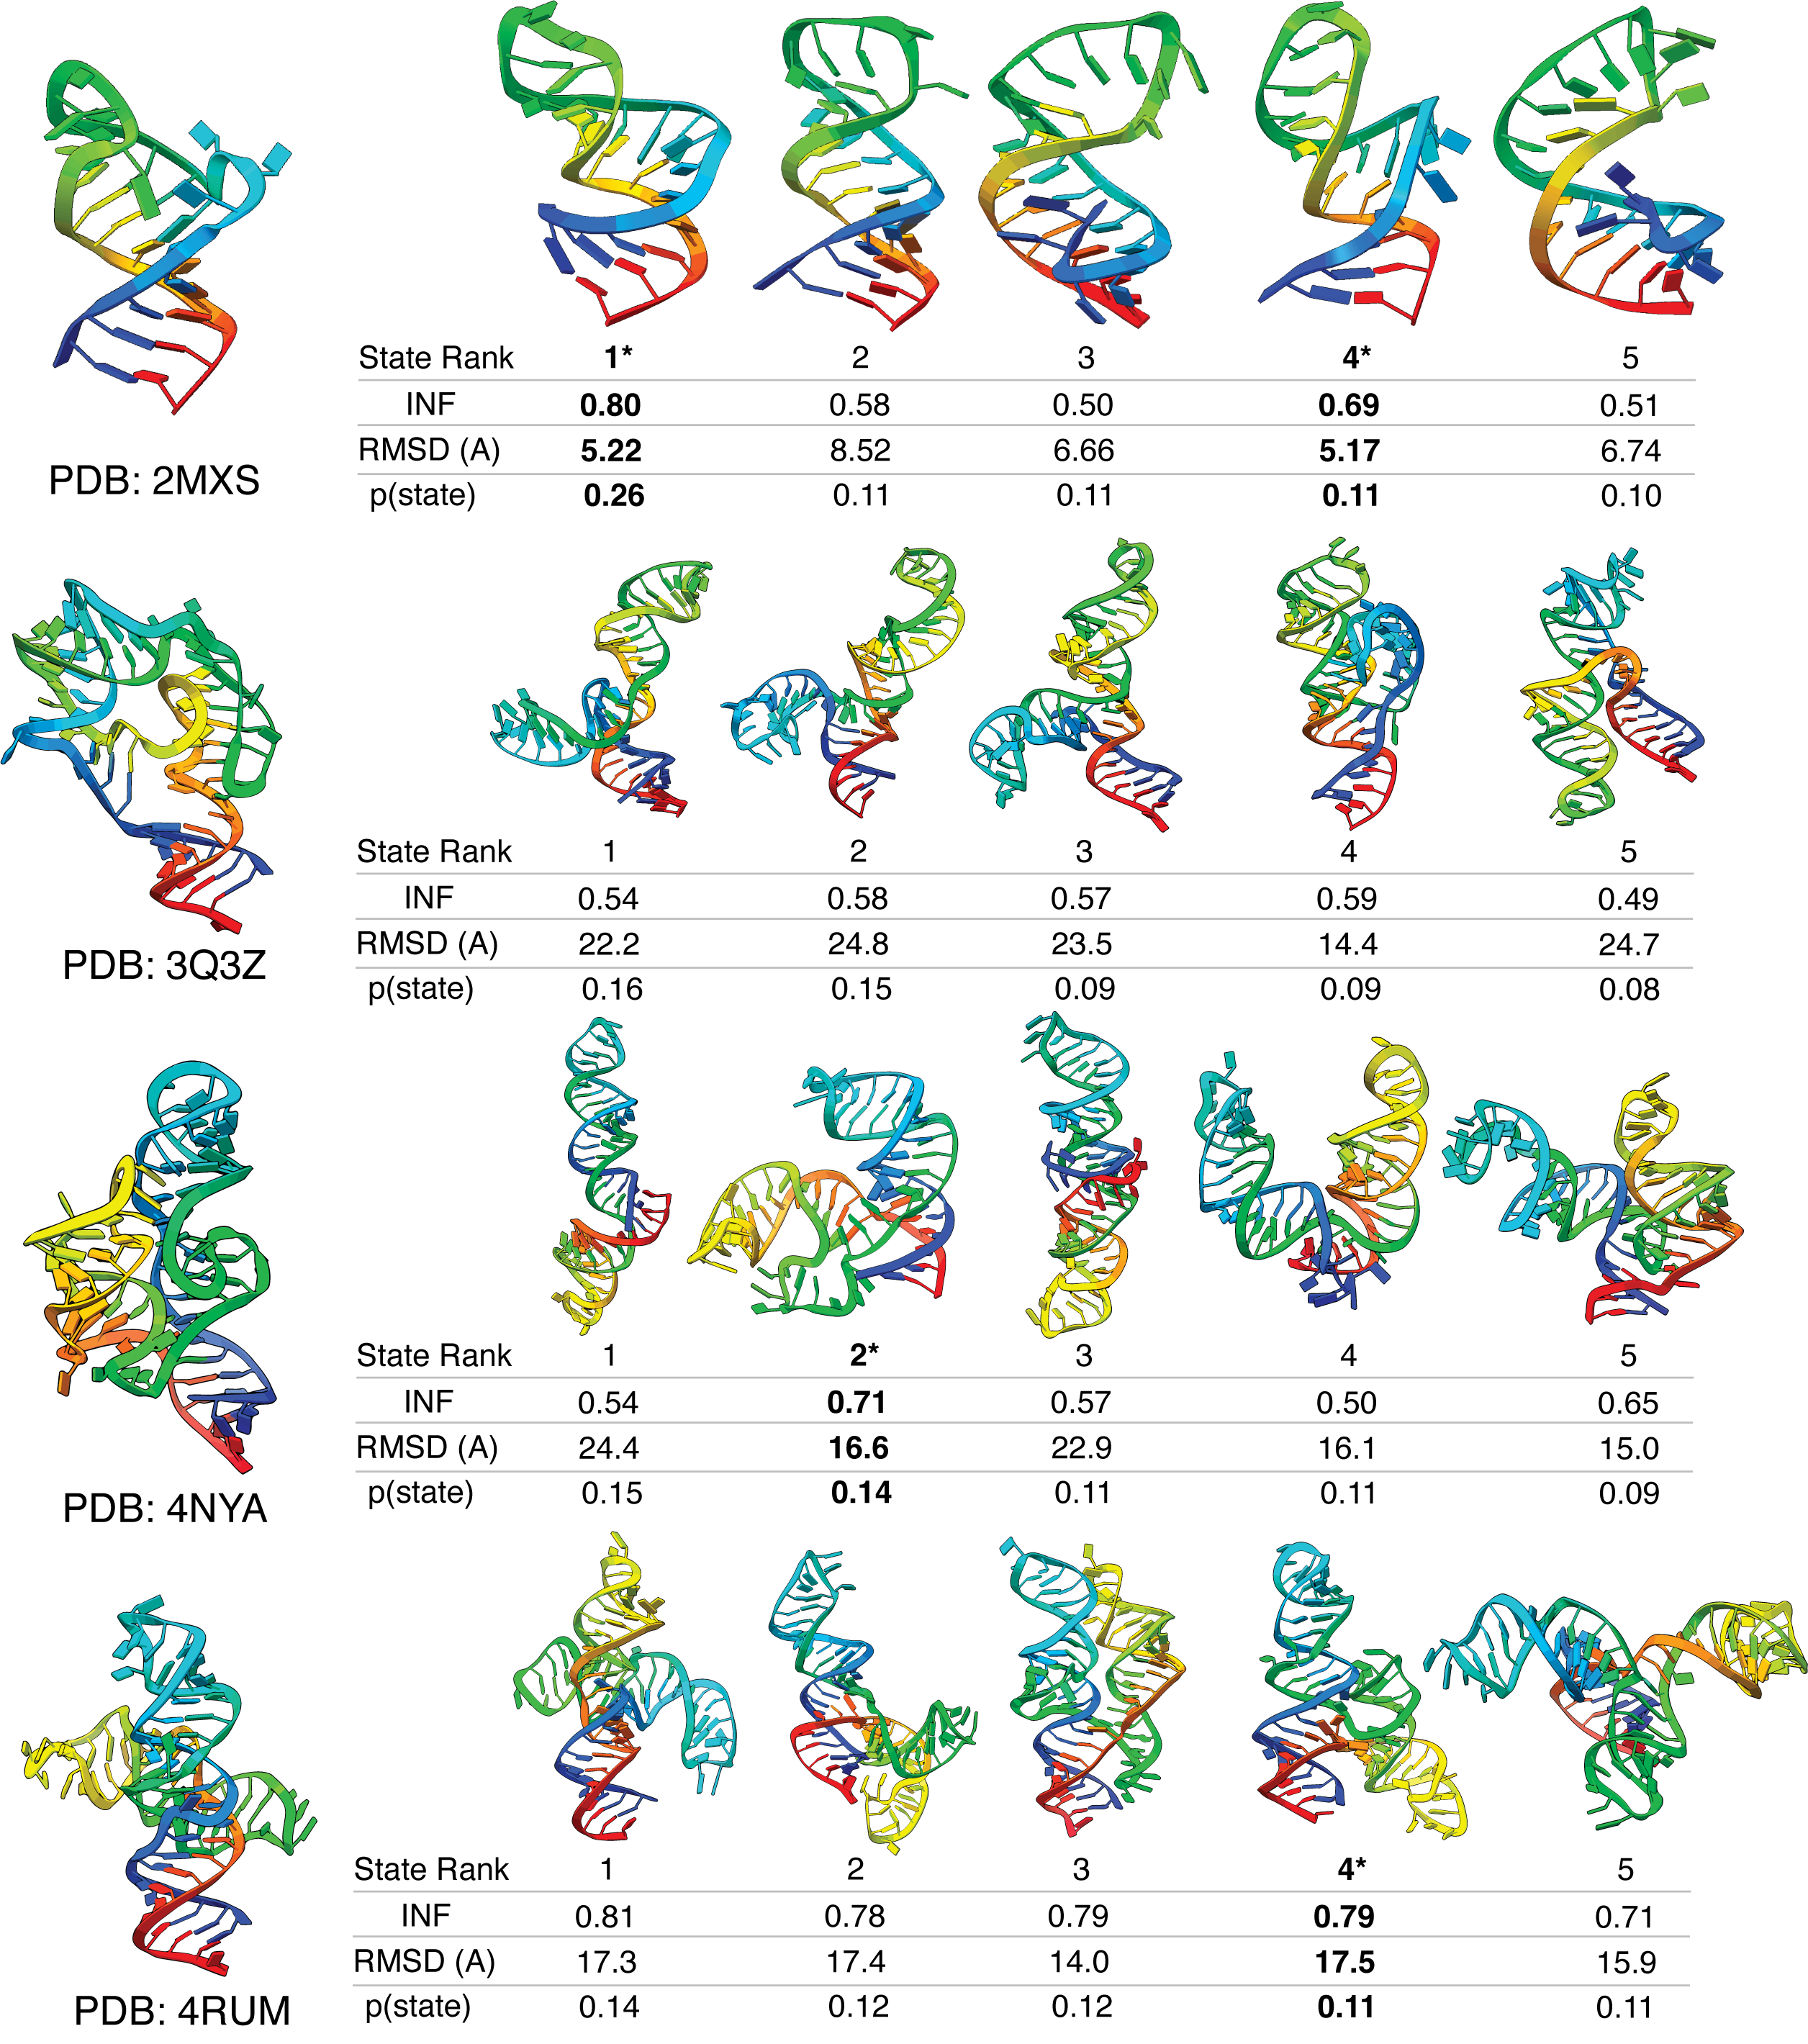
\includegraphics[
    width=\textwidth
    ]{./rep-ensemble-1.png}
    \caption{{\bf Conformational ensembles predicted by RNAnneal (2MXS, 3Q3Z, 4NYA, 4RUM)}. The five most probable states are reported alongside their probabilities. The best scoring model from each state is shown as a representative conformation, and the INF and RMSD values compared to the experimentally-resolved conformation (left) are reported.}
    \label{fig:rep-ensemble-1}%
\end{figure*}

\begin{figure*}
    \centering
    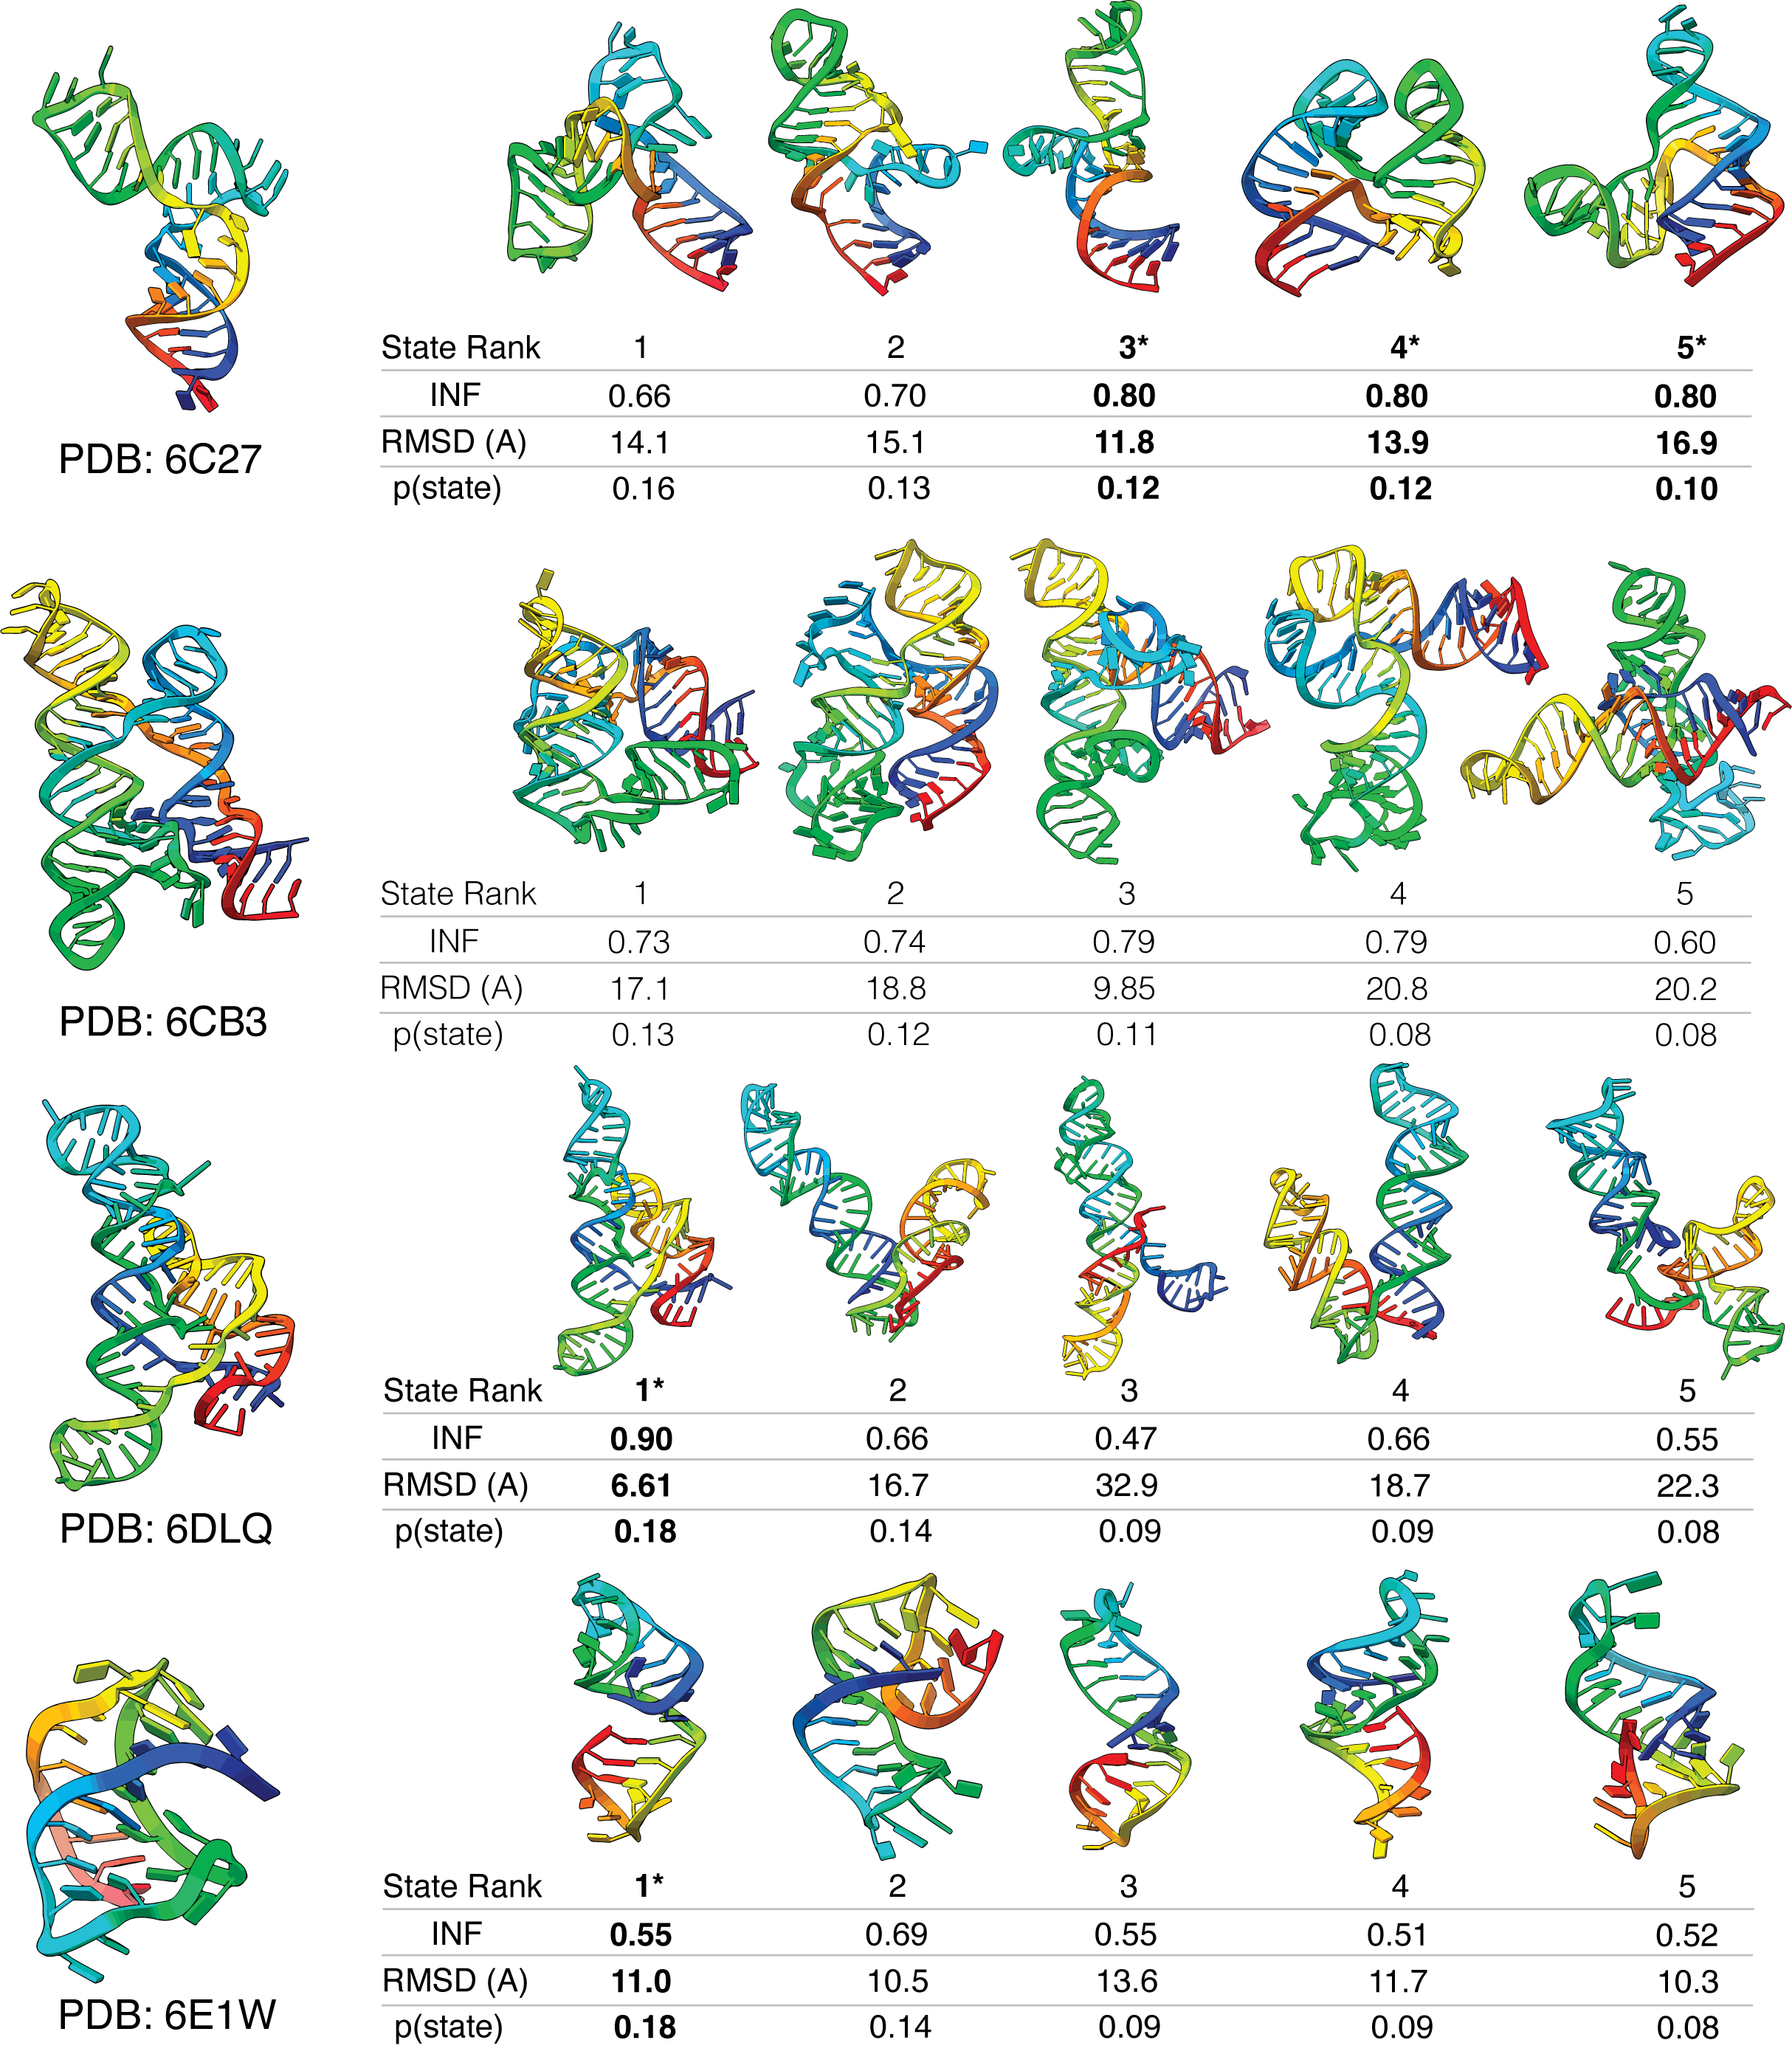
\includegraphics[
    width=\textwidth
    ]{./rep-ensemble-2.png}
    \caption{{\bf Conformational ensembles predicted by RNAnneal (6C27, 6CB3, 6DLQ, 6E1W)}. The five most probable states are reported alongside their probabilities. The best scoring model from each state is shown as a representative conformation, and the INF and RMSD values compared to the native-like conformation (left) are reported.}
    \label{fig:rep-ensemble-2}%
\end{figure*}

\begin{figure*}
    \centering
    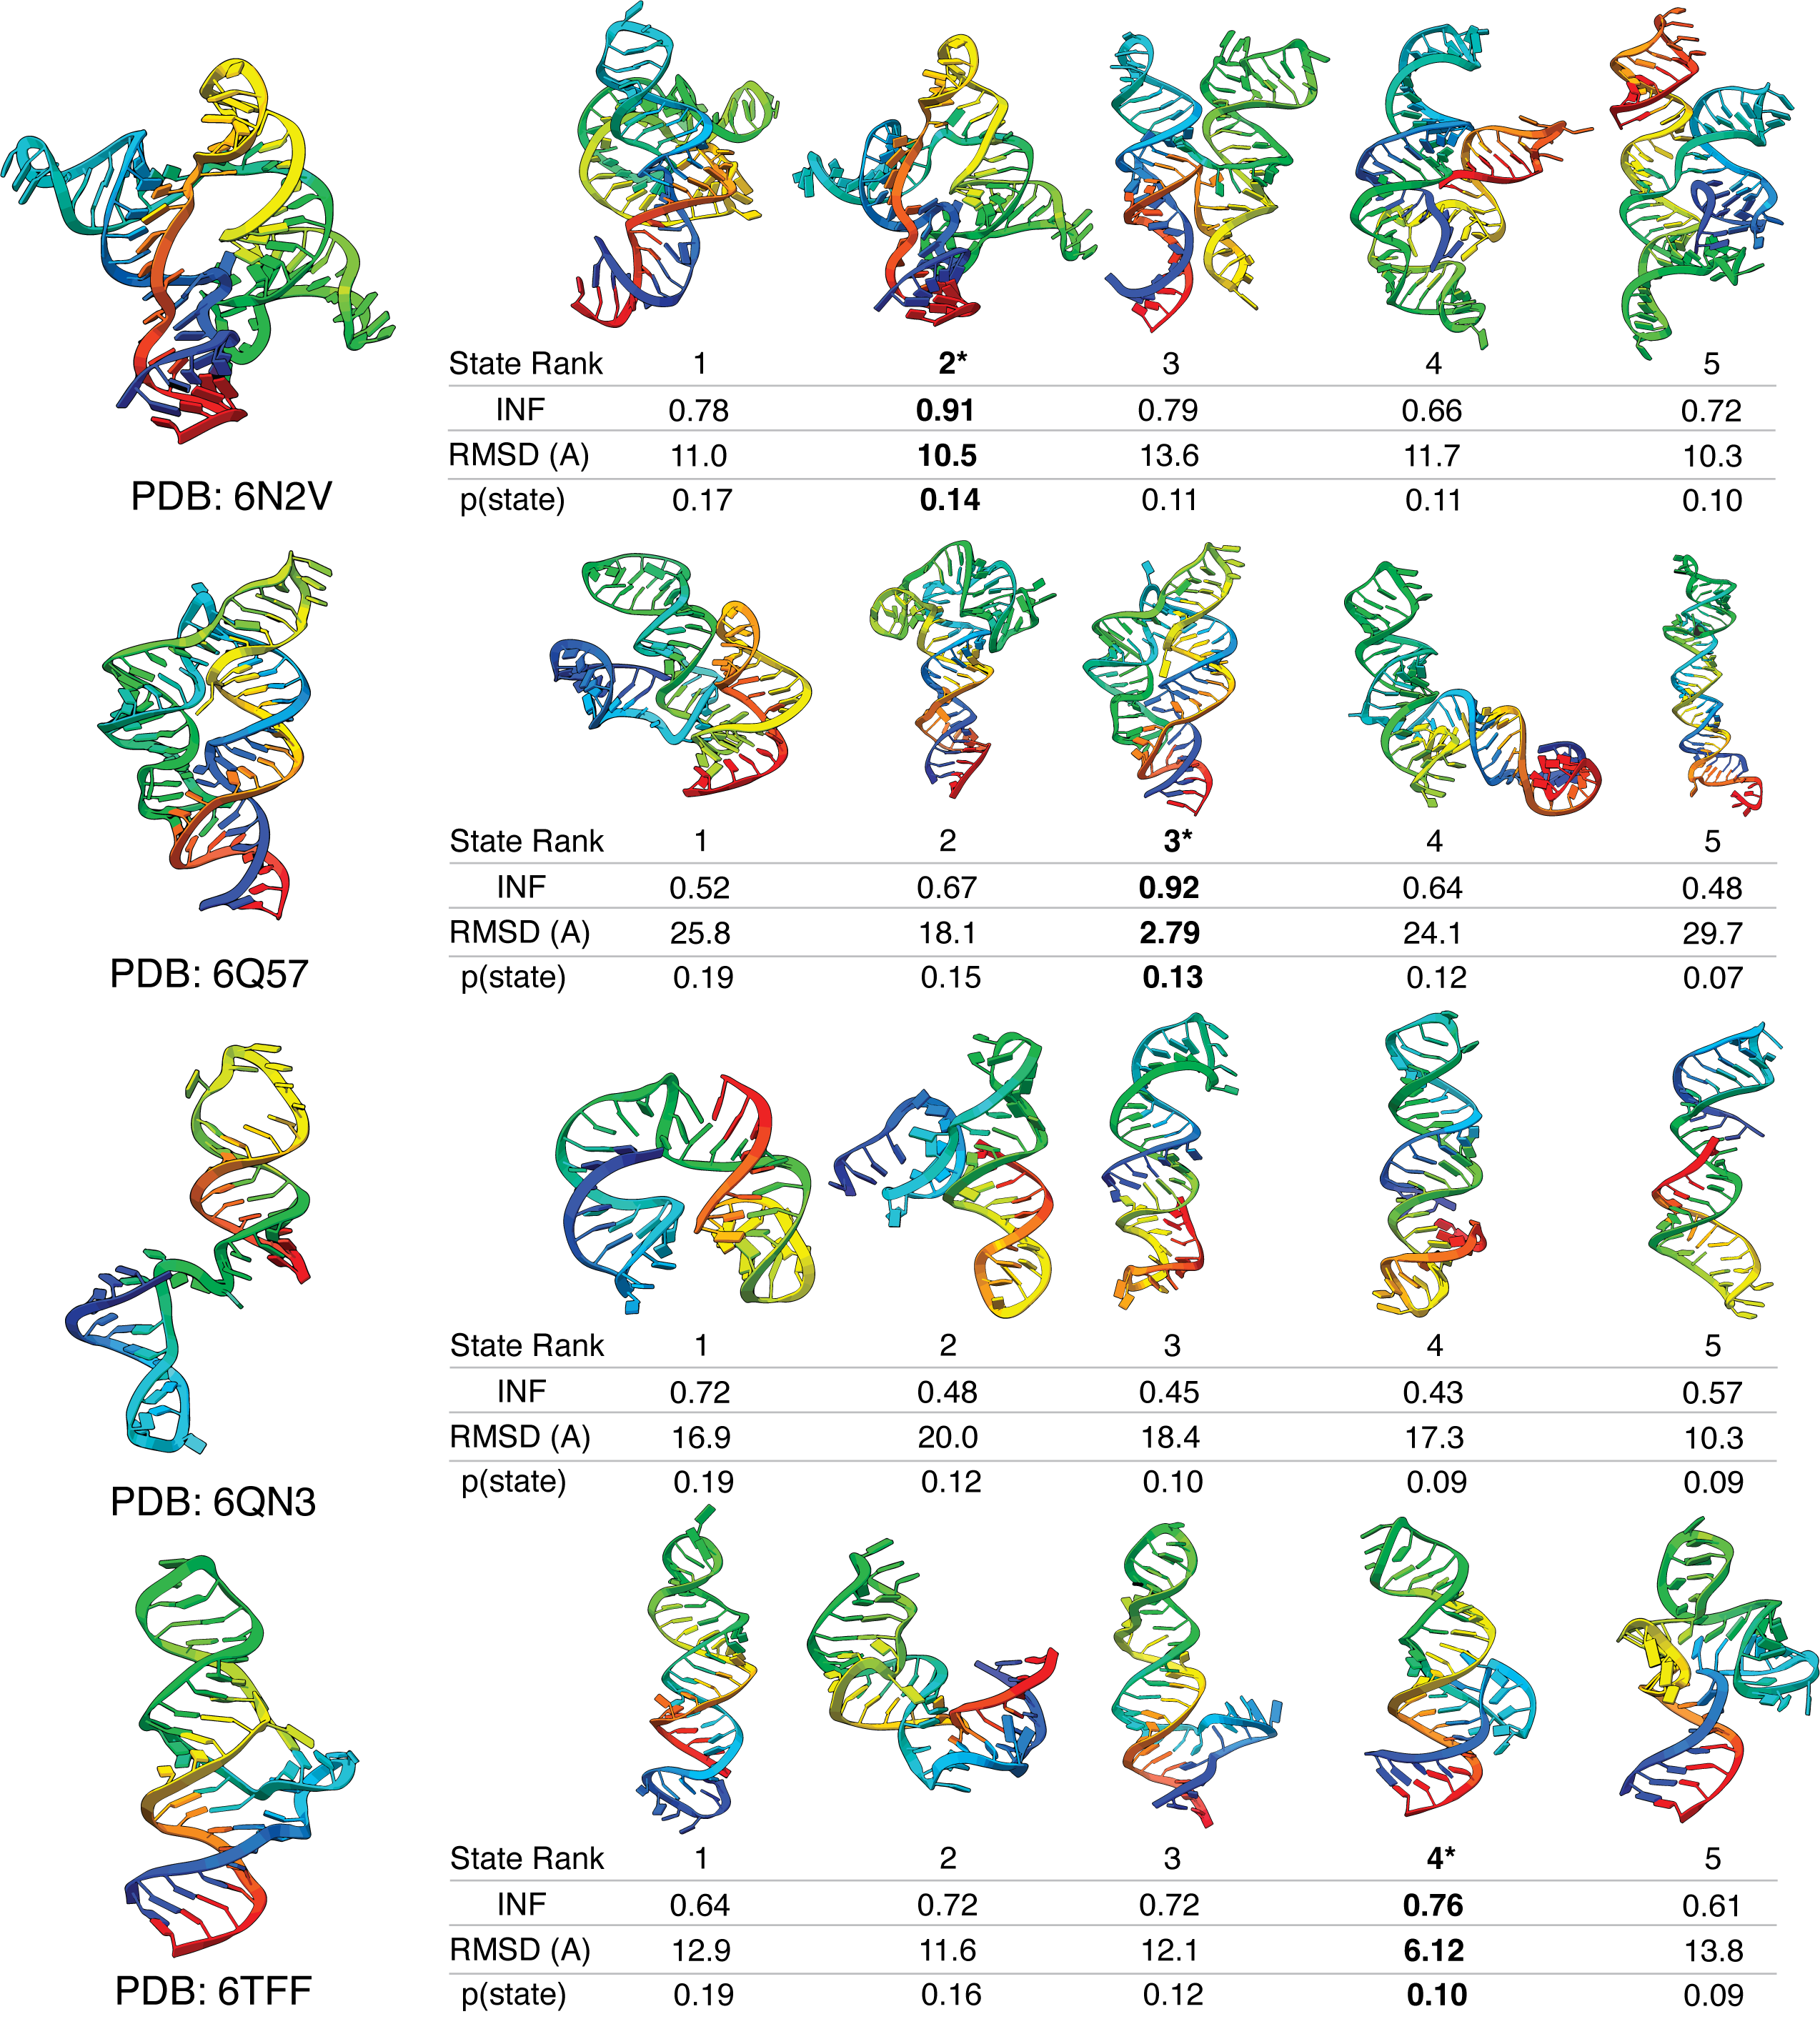
\includegraphics[
    width=\textwidth
    ]{./rep-ensemble-3.png}
    \caption{{\bf Conformational ensembles predicted by RNAnneal (6N2V, 6Q57, 6QN3, 6TFF)}. Experimentally solved structures for each RNA are depicted to the left. The five most probable states are reported alongside their probabilities. The best scoring model from each state is shown as a representative conformation, and the INF and RMSD values compared to the native-like conformation are reported.}
    \label{fig:rep-ensemble-3}%
\end{figure*}

\begin{figure*}
    \centering
    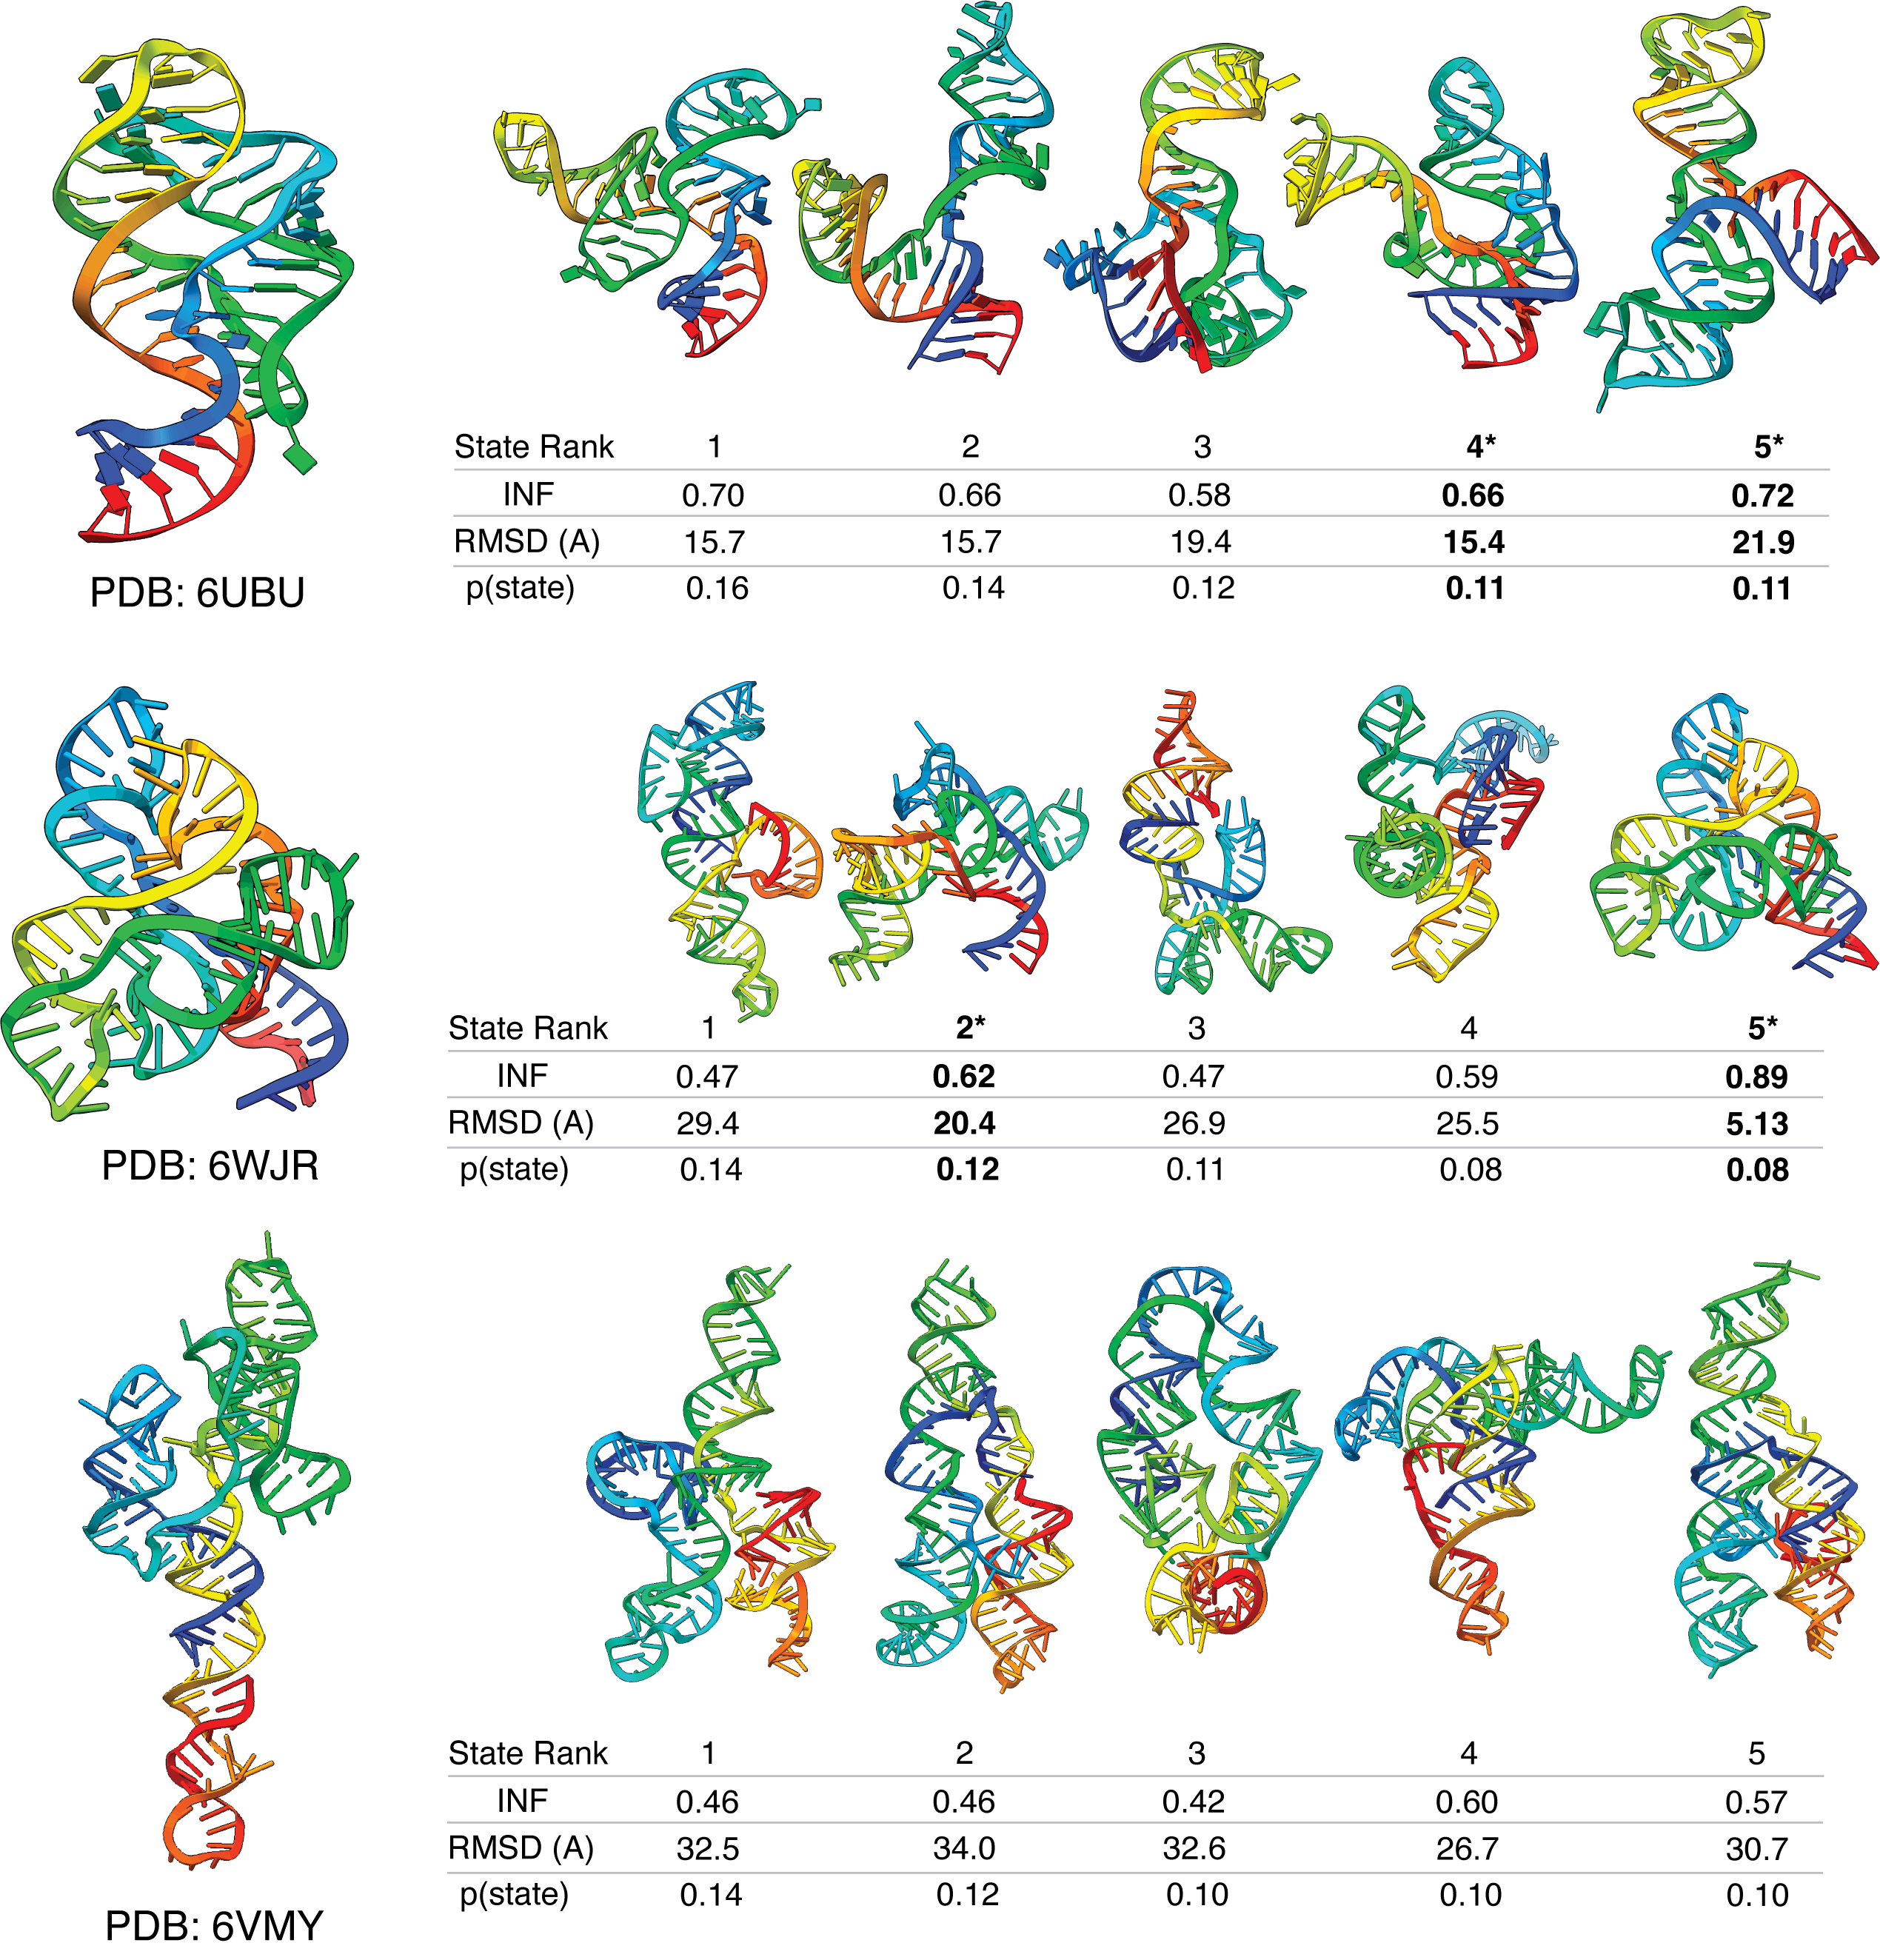
\includegraphics[
    width=\textwidth
    ]{./rep-ensemble-4.png}
    \caption{{\bf Conformational ensembles predicted by RNAnneal (6UBU, 6WJR, 6VMY)}. Experimentally solved structures for each RNA are depicted to the left. The five most probable states are reported alongside their probabilities. The best scoring model from each state is shown as a representative conformation, and the INF and RMSD values compared to the native-like conformation are reported.}
    \label{fig:rep-ensemble-4}%
\end{figure*}

\begin{table}[ht]
  \centering
  \begin{tabular}{@{} l c c c c c c @{}}
    \toprule
    \textbf{RNA} 
      & \textbf{PDB} 
      & \makecell[l]{\textbf{Monomer}}
      % & \textbf{Apo/Holo}
      & \makecell[l]{\textbf{State}}
      & \textbf{Length} 
      & \textbf{Sequence} 
      & \textbf{Secondary Structure} \\
    \midrule
    
    \addlinespace[0.5em]


    % first row
    \makecell[l]{Neomycin \\ sensing \\ riboswitch}
    & 2MXS\cite{Ramesh2014}
    & Y
    & Holo
    & 28
    & \makecell[l]{%
          \texttt{ggcugcuuguccuuuaaugguccaguc}
        }
    & \makecell[l]{
      \texttt{(.(((...(.((......)).)))).)}
      } \\

    \addlinespace[0.5em]

    % second row
    \makecell[l]{c‑di‑GMP‑II \\ riboswitch}
    & 3Q3Z\cite{Smith2010}
    & Y
    & Holo
    & 76
    & \makecell[l]{%
          \texttt{gcgcggaaacaaugaugaauggguuuaaau}  \\
          \texttt{ugggcacuugacucauuuugaguuaguagu} \\
          \texttt{gcaaccgaccgugcu}
          }
    & \makecell[l]{
      \texttt{((.(((..((.......((((.((......}\\
      \texttt{[\{\{[[[[[..)).))))....))....]]]}\\
      \texttt{]]].\}\}..))).)).}
      }
      \\

    \addlinespace[0.5em]

    \makecell[l]{TPP \\ riboswitch}
    & 4NYA\cite{Warner2014}
    & Y
    & Holo
    & 81
    & \makecell[l]{%
          \texttt{ggacucggggugcccuucugcgugaaggcu} \\
          \texttt{gagaaauacccguaucaccugaucuggaua} \\ 
          \texttt{augccagcguagggaaguuc} \\
        }
      
    & \makecell[l]{
    \texttt{(.(((((((.((((.(((.....)))))).}\\
    \texttt{.....)..)))).....(((...((((...}\\
    \texttt{...))))...)))..))).)}
      }
      \\

        \addlinespace[0.5em]

    \makecell[l]{NiCo \\ transition\\-metal \\ riboswitch}
    & 4RUM\cite{Warner2014}
    & Y
    & Holo
    & 93
    & \makecell[l]{%
          \texttt{gggaacugagcaggcaaugaccagagcggu} \\
          \texttt{caugcagccgggcugcgaaagcggcaacag} \\
          \texttt{augauacacgcacaucugugggacaguucc} \\
          \texttt{ca}
        }

    & \makecell[l]{
    \texttt{((((((((..(.(((.((((((.....)))} \\
    \texttt{)))...)))..((.((....)).)).((((} \\
    \texttt{(((.........)))))))..).)))))))} \\
    \texttt{).}
      }
      \\

    \addlinespace[0.5em]

    \makecell[l]{SAM-III \\ riboswitch}
    & 6C27\cite{Grigg2018}
    & Y
    & Holo
    & 48
    & \makecell[l]{%
          \texttt{gggacaaguucccgaaaggauggcggaaac} \\
          \texttt{gccagaugccuuguccc} \\
        }

    & \makecell[l]{
    \texttt{.(((((((.(.(.....).)(.((......} \\
    \texttt{)).).....))))))).} \\
      }
      \\

    \addlinespace[0.5em]

    \makecell[l]{YkoY\\riboswitch}
    & 6CB3\cite{Bachas2018}
    & N
    & Holo
    & 100
      & \makecell[l]{%
          \texttt{aaaggggaguagcgucgggaaaccgaaaca} \\
          \texttt{aagucgucaauucgugaggaaacucaccgg} \\
          \texttt{cuuuguugacauacgaaaguauguuuagca} \\
          \texttt{agaccuuuc} \\
        }
      & \makecell[l]{
    \texttt{.((((......((.((((....))))((((} \\
    \texttt{(((.((.......(((((....))))))).} \\
    \texttt{))))))).((((((....))))))...)).} \\
    \texttt{...))))..} \\
      }
      \\

    \addlinespace[0.5em]

    \makecell[l]{PRPP \\ riboswitch}
    & 6DLQ\cite{Bachas2018}
    & Y
    & Holo
    & 108
    & \makecell[l]{%
          \texttt{ggaaagugugucuaggguuccgcgugcuuc} \\
          \texttt{ggcacggacugguccaagugacacagacgc} \\
          \texttt{auucgugcguuacaccggagggauagaagc} \\
          \texttt{ccaggcggguagguuuc} \\
        }
    & \makecell[l]{
    \texttt{..((...(((((..((...((.(((((...} \\
    \texttt{.)))))....)).))....)))))..((((} \\
    \texttt{(....)))))..(.[[[..(((.......)} \\
    \texttt{)).).]]]......)).} \\
      }
      \\

    \addlinespace[0.5em]

    \makecell[l]{PreQ1 \\ riboswitch}
    & 6E1W\cite{Numata2019}
    & Y
    & Holo
    & 31
    & \makecell[l]{%
          \texttt{cugggucgcaguuuccccaguuaacaaaac}
        }
    & \makecell[l]{
    \texttt{(((((.....[....))))).........]}
      }
      \\

    \addlinespace[0.5em]

    \makecell[l]{Mn$^{2+}$-\\sensing \\ riboswitch}
    & 6N2V\cite{Price2018}
    & Y
    & Holo
    & 99
    & \makecell[l]{%
          \texttt{gcuuggggaguagccugcuuucggaaacga} \\
          \texttt{aagcgccuguaucaacauacucggcgaaag} \\
          \texttt{ccguggugcaggaccgaaaggucuggcgag} \\
          \texttt{accaggcc}
        }

    & \makecell[l]{
    \texttt{.(.(((......(((..(.((((....)))} \\
    \texttt{).)..((((.(.((.......((((....)} \\
    \texttt{))))).).))))(((....)))..)))...} \\
    \texttt{.))).)..} \\
      }
      \\

    \addlinespace[0.5em]

    \makecell[l]{Tetrahydro-\\folate \\ riboswitch}
    & 6Q57\cite{Dunstan2018}
    & Y
    & Holo
    & 90
    & \makecell[l]{%
          \texttt{ggagaguagaugauucgcguuaagugugug} \\
          \texttt{ugaaugggaugucgucacacaacgaagcga} \\
          \texttt{gagcgcggugaaucauugcauccgcucca} \\
        }
      
    & \makecell[l]{
    \texttt{.(((......((((((.((.......((((} \\
    \texttt{(((...[[[[[...)))))))....((...} \\
    \texttt{.)).))..))))))...]]]]].)))..} \\
      }
      \\

    \addlinespace[0.5em]

    \makecell[l]{Glutamine \\ II riboswitch}
    & 6QN3\cite{Huang2019}
    & N
    & Holo
    & 51
    & \makecell[l]{%
          \texttt{cguucacccuucggggcgcaugaaauggga} \\
          \texttt{guagggaacgggauucucau}
        }
    & \makecell[l]{
    \texttt{......(((....)))........(.(.((} \\
    \texttt{.(..........).)).).)} \\
      }
      \\

    \addlinespace[0.5em]

    \makecell[l]{NAD$^{+}$ \\ riboswitch}
    & 6TFF\cite{Huang2020}
    & Y
    & Holo
    & 53
    & \makecell[l]{%
          \texttt{ggcuucaacaaccccguagguugggccgaa} \\
          \texttt{aggcagcgaaucuacuggagcc}
        }
    & \makecell[l]{
    \texttt{((((.((.....[[.((((.(((.(((...} \\
    \texttt{.))).]]))).)))))).))))} \\
      }
      \\

    \addlinespace[0.5em]

    \makecell[l]{Guanine\\ riboswitch}
    & 6UBU\cite{Matyjasik2019}
    & Y
    & Holo
    & 68
    & \makecell[l]{%
          \texttt{ggacauauaaucgcguggauauggcacgca} \\
          \texttt{aguuucuaccgggcaccguaaauguccgac} \\
          \texttt{uaugucc}
        }

    & \makecell[l]{
    \texttt{((((((((..(.(((((.....[[))))).} \\
    \texttt{)[.....)](((.((]].....)).)))..} \\
    \texttt{)))))))} \\
      }
      \\

    \addlinespace[0.5em]

    \makecell[l]{FMN \\ riboswitch}
    & 6WJR\cite{Wilt2020}
    & Y
    & Apo
    & 112
    & \makecell[l]{%
          \texttt{ggaucuucggggcagggugaaauucccgac} \\
          \texttt{cggugguauaguccacgaaaguauuugcuu} \\
          \texttt{ugauuuggugaaauuccaaaaccgacagua} \\
          \texttt{gagucuggaugagagaagauu}
        }
    & \makecell[l]{
    \texttt{..((((((.......((.......))..((} \\
    \texttt{((((((....[[))))..(((......)))} \\
    \texttt{...(((((.......)))))]])).[[[..} \\
    \texttt{..))]]].......)))))).} \\
      }
      \\
    
    \addlinespace[0.5em]

    \makecell[l]{Cobalamin \\ riboswitch}
    & 6VMY\cite{Chan2020}
    & Y
    & Holo
    & 149
    & \makecell[l]{%
          \texttt{ggucaaauaggugccgguccgugaacaaca} \\
          \texttt{gccggcuuaaaagggaaaccgguaaaagcc} \\
          \texttt{ggugcggucccgccacuguaauuggccaag} \\
          \texttt{cgccaagagccaggauaccugccuguuuga} \\
          \texttt{ucagcacgaauucugcgaggacagauga}
        }
    & \makecell[l]{
    \texttt{(.((.((.(((.(((((..[((.....)).} \\
    \texttt{.))))).....(((....((((......))} \\
    \texttt{)).((((.....)).[[[....((((....} \\
    \texttt{.))))...))]]]]...))).))).)).))} \\
    \texttt{.)..(.....((........).)...).} \\
      }
      \\


    \bottomrule
  \end{tabular}
  \caption{Details of riboswitch sequences and reference conformations}
  \label{tab:riboswitches}
\end{table}

\begin{table}[]
  \centering
  \begin{tabular}{lccc}
    \toprule
    \textbf{Stage} & \textbf{Duration (ps)} & \textbf{Timestep (fs)} & \textbf{Temperature (K)} \\
    \midrule
    Equilibration 1   &     1    &  0.1 &   1   \\
    Equilibration 2.1 &     1    &    1 &  10   \\
    Equilibration 2.2 &     1    &    1 &  20   \\
    Equilibration 2.3 &     1    &    1 &  30   \\
    Equilibration 2.4 &     1    &    1 &  40   \\
    Equilibration 2.5 &     1    &    1 &  50   \\
    Equilibration 3.1 &     2    &    1 & 100   \\
    Equilibration 3.2 &     2    &    1 & 150   \\
    Equilibration 3.3 &     2    &    1 & 200   \\
    Equilibration 3.4 &     2    &    1 & 250   \\
    Equilibration 3.5 &     2    &    1 & 300   \\
    Equilibration 4.1 &    20    &    1 & 300   \\
    Equilibration 4.2 &    20    &    2 & 300   \\
    Equilibration 4.3 &    20    &    3 & 300   \\
    Equilibration 4.4 &    20    &    4 & 300   \\
    Equilibration 4.5 &    20    &    5 & 300   \\
    Production        & 100{,}000 &    5 & 300   \\
    \bottomrule
  \end{tabular}
    \caption{Molecular Dynamics Equilibration Procedure}
  \label{tab:schedule}
\end{table}

\begin{table}[]
  \centering
  \begin{tabular}{ll}
    \toprule
    \textbf{Parameter}            & \textbf{Value}                    \\
    \midrule
    Simulation Engine             & OpenMM                            \\
    Ion Type                      & NaCl                              \\
    Ion Concentation              & 1 M                                \\
    Box Shape                     & Dodecahedron                      \\
    Box Padding                   & 0.5 nm                            \\
    Force Field (Solute)           & RNA.Shaw\_charmm22-ions.xml       \\
    Force Field (Solvent)          & implicit/gbn2.xml                 \\
    Pressure                      & 1 atm                             \\
    Sampling Frequency            & 1 ns                              \\
    \bottomrule
  \end{tabular}
  \caption{Molecular Dynamics Simulation Parameters.}
\label{tab:parameters}
\end{table}






\end{document}